\documentclass{article}
\usepackage{graphicx}
\usepackage{amsmath}
\usepackage{hyperref}
\usepackage{float}

% package for including polish language in the document
\usepackage[utf8]{inputenc}
%\usepackage[polish]{babel}

\title{Evolution of suicides in Poland in the last two decades}

\begin{document} 

\maketitle

\section{Introduction}
%
The data used in this analysis come from the website of the Polish National
Police, available at 
\url{https://statystyka.policja.pl/st/wybrane-statystyki/zamachy-samobojcze}. 
The data are divided into three ranges of years: from 1999 to 2012,
from 2013 to 2016 and from 2017 to 2023, some discrepancies in the format
were inevitably present and fortunately easy to fix.
In every range of years, the data are provided in different excel files,
each file focusing on a different aspect,
here follows a list of the files for each range of years.
\begin{itemize}
\item Age range (grupa wiekowa) and day of the week (dzień tygodnia)(the day of the week is not 
treated in this writing).
\item Place where the deed took place (miejsce popełnienia), also containing
the subdivision into men (w tym mężczyzn) and women (w tym kobiet),
unfortunately the subdivision is not made for every place where 
the corpses were found but it only regards the total values, that is,
it is not reported for a specific place how many were the women and how many were
the men found there.
\item Method used (sposób popełnienia), 
reason for the deed  (powód popełnienia), the two \textit{variables}
are treated separately, e.g. it is not possible to know how many people
that committed suicide for a specific reason adopted a specific method.
Again, this file contains the same information on the sex of the victimi as in
the previous file but
this information is not reported for every specific reason or method.
\item Civil status (stan cywilny), education (wykształcenie),
job (informacja o pracy/nauce), these \textit{variables} are treated
separately (that is, it is not reported for a specifi education level how many were the 
people that committed suicide that worked in a specific area)
and the same goes again for the information on sex.
\end{itemize}
The 4 files are published in couples: one reports the information on
attempted suicides (zamachy samobójcze) and the other reports 
the attempted suicides resulting in death (zamachy samobójcze zakończone
zgonem).
Other data regarding the source of income (żródło utrzymania),
state of consciousness (stan świadomości),
mental state (stan psychiczny) and criminal history (przeszłość karna)
are available but they are not treated in this article. \\
Each of these files displays data by rows, where every row focuses on a specific country
and a specific year, this format is not the one commonly adopted and referred to as
\textit{tabular data}, where every variable is a column. 
The preparation of data is available at: 
\url{https://www.kaggle.com/code/denisfesta/preparation-of-data-on-suicides-in-poland},
where the code is available to see how the \texttt{excel} files were translated into 
\texttt{csv} files with a tabular format.
%
% SCREENSHOT OF THE EXCEL FILE AND THE
% CLEANED DATA SIDE BY SIDE
%

\section{Global view}
Figures \ref{fig:poland_general} and \ref{fig:poland_foa} show the evolution of the the 
number of suicides in Poland from 1999 to 2022 and the ratio of the suicides resulting
in death over the total number of attempts, respectively.
\begin{figure}[H]
	\centering
	\begin{minipage}{0.55\textwidth}
		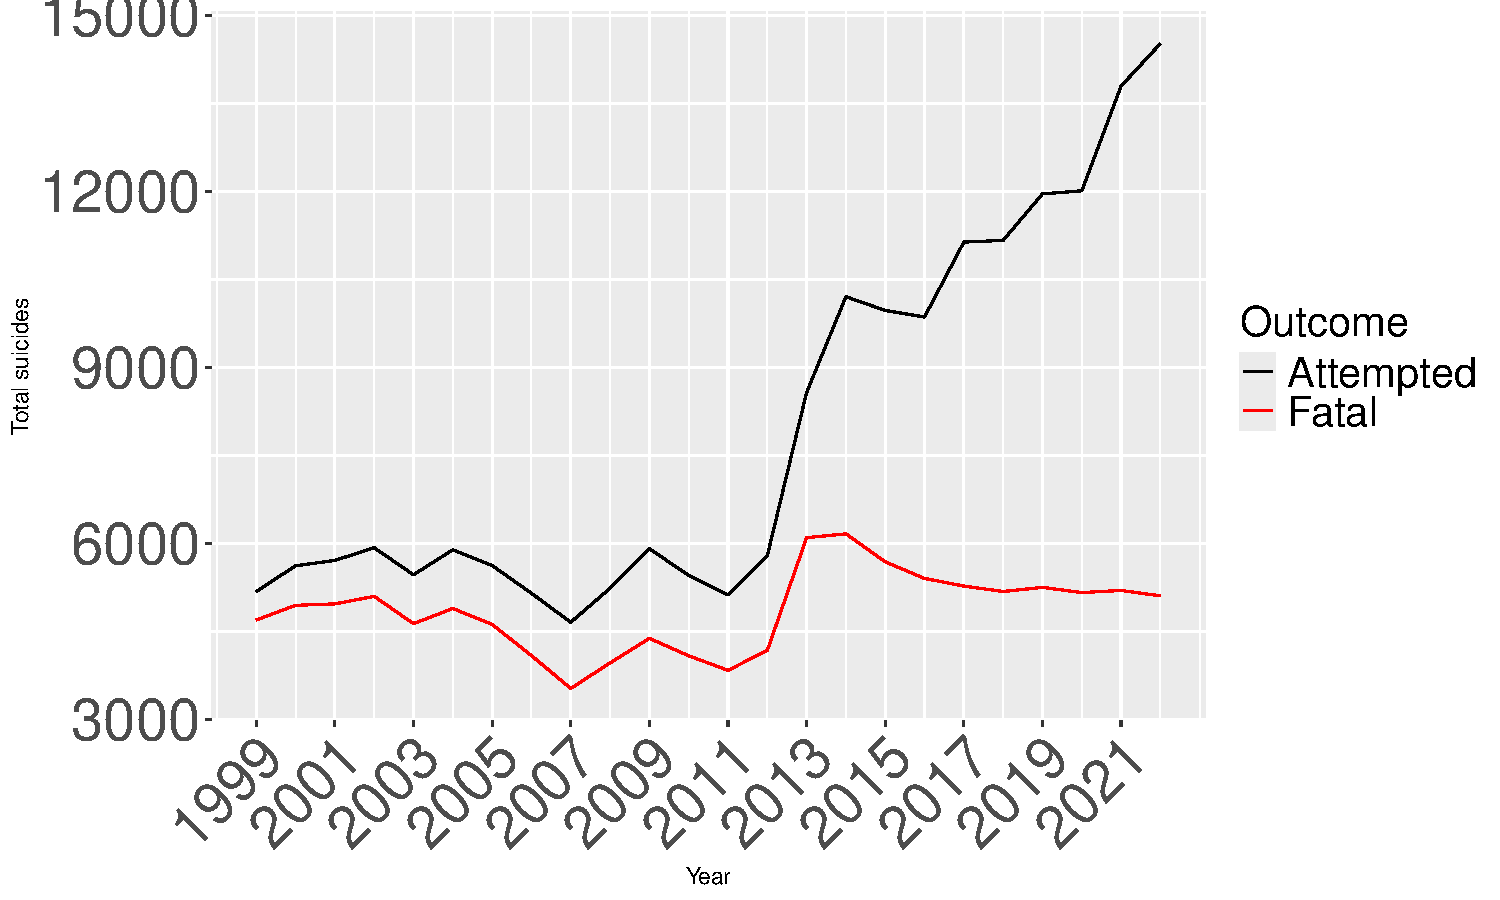
\includegraphics[width=\textwidth]{imgs/poland_general.pdf}
		\caption{The evolution of the suicides (attempts and deaths) in Poland}
		\label{fig:poland_general}
	\end{minipage}
	\hfill
	\begin{minipage}{0.55\textwidth}
		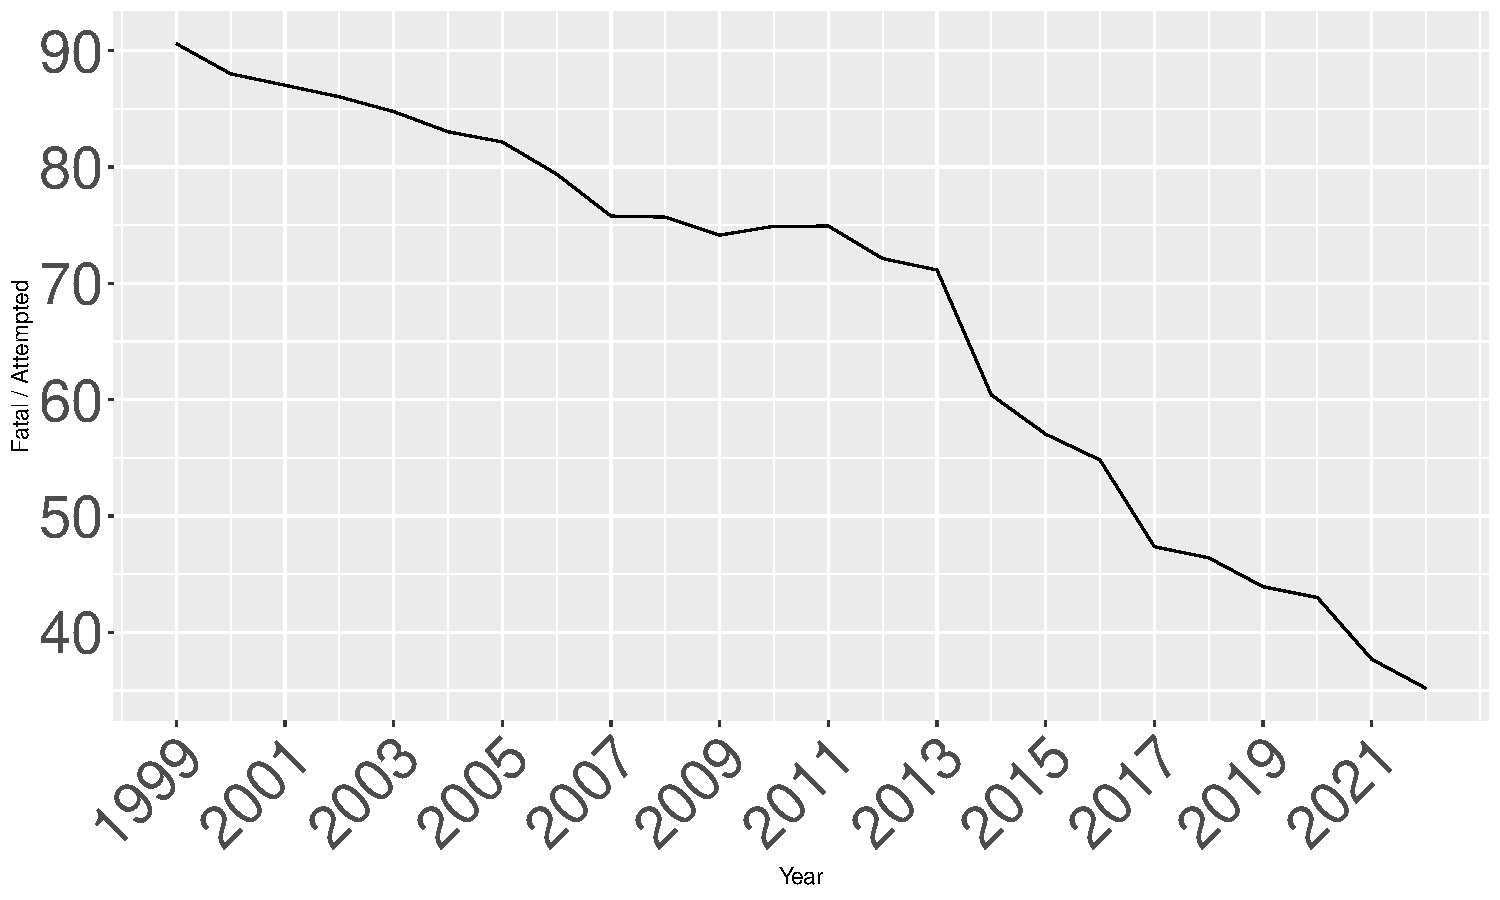
\includegraphics[width=\textwidth]{imgs/poland_foa.pdf}
		\caption{The ratio of the suicides resulting in death over the total number of attempts}
		\label{fig:poland_foa}
	\end{minipage}
\end{figure}
The abrupt increase in the suicide attempts just before 2013 is more due to to a technical 
reason rather than a real increase in the number of attempts,
as reported on the main page of the website:
\begin{quote}
	\textit{Since 2013, the method of collecting and generating statistical data 
	on suicide attempts has changed. Currently, data are entered into KSIP via 
	form KSIP 10 – “Registration of a suicide attempt report” immediately after 
	the event at the moment it is determined that a suicide attempt has occurred. 
	Additionally, the system “freezes” the data with a one-month delay, allowing 
	for modifications in cases where it is determined at a later stage of the 
	procedure that a suicide attempt did not occur.}
\end{quote}
The change in how attempted suicides are reported might explain why, from around 2015, 
the trend of attempted suicides shows a different behaviour
that does not resemble the one of the trend of fatal suicides.  \\ \\
%
%
The unfortunate increment between 2012 and 2013 in the number of fatal suicides cannot be simply justified
by the technical reason reported above. \\
%
%
% INCOME
%
One quantity whose trend might be relevant to compare to that of the suicides
is the income but, as shown in the following graphs
(\ref{fig:income}), it does not seem to bring
relevant justifications since it is only increasing during the years.
%
%
% EMPLOYMENT
%
Another possibly relevant quantity is the employment ratio (\ref{fig:employment}), unfortunately the only available data
start from 2010. The naive assumption initially made was that people aged between 30 and 50 are more likely
to commit suicide because of unemployment. The increase of suicides between 2012 and 2013 is 
present also for that range of age and it looks correlated to the decrease in the employment
ratio.

\begin{figure}[H]
	\centering
	\begin{minipage}{0.45\textwidth}
		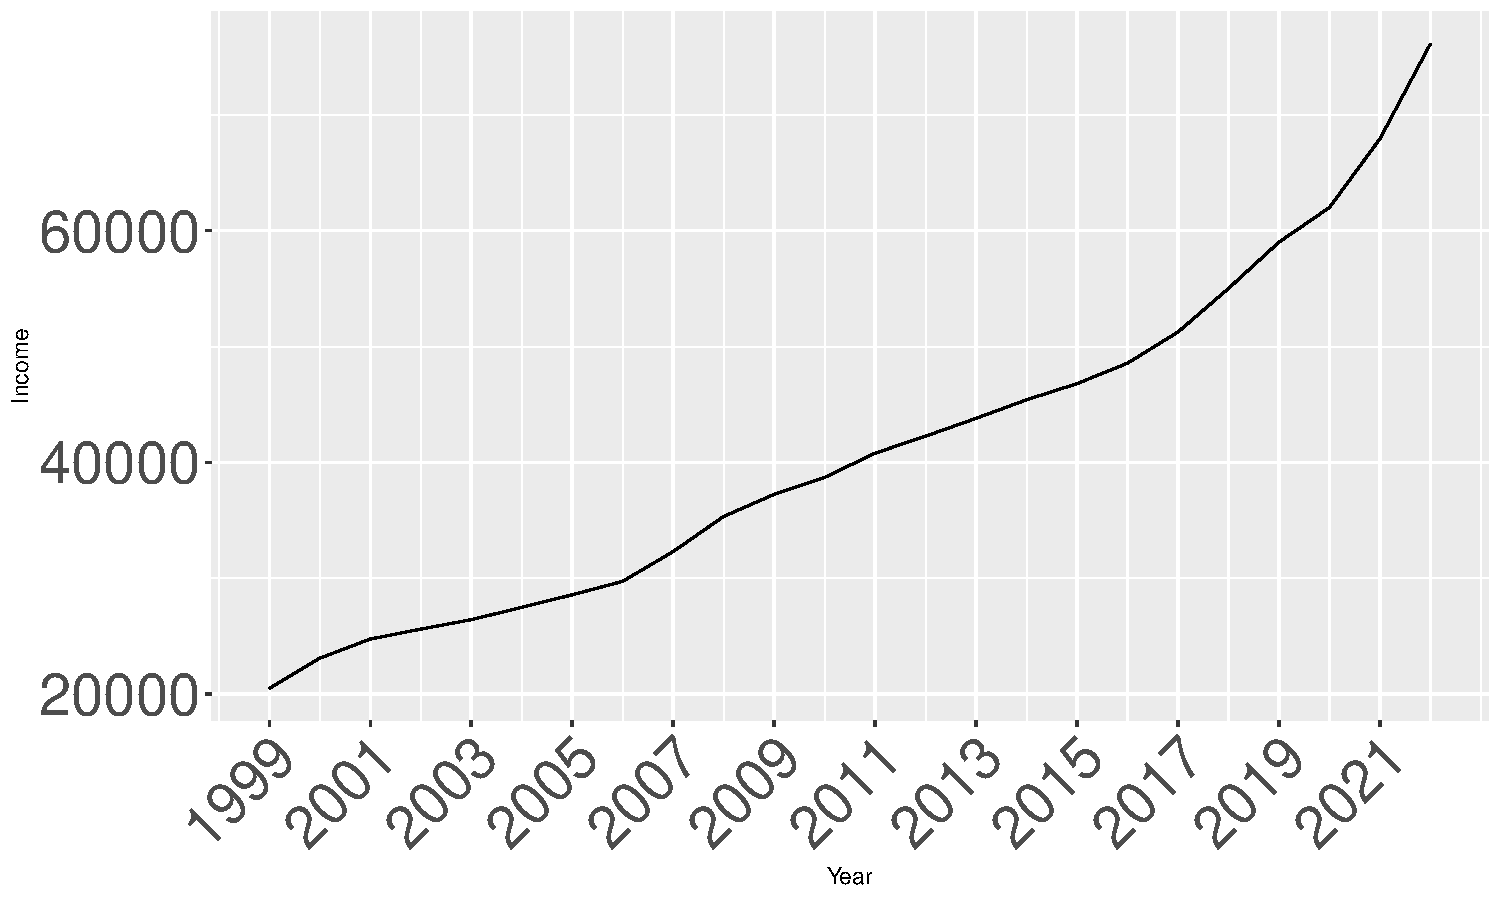
\includegraphics[width=\textwidth]{imgs/income.pdf}
		\caption{The income}
		\label{fig:income}
	\end{minipage}
	\hfill
	\begin{minipage}{0.45\textwidth}
		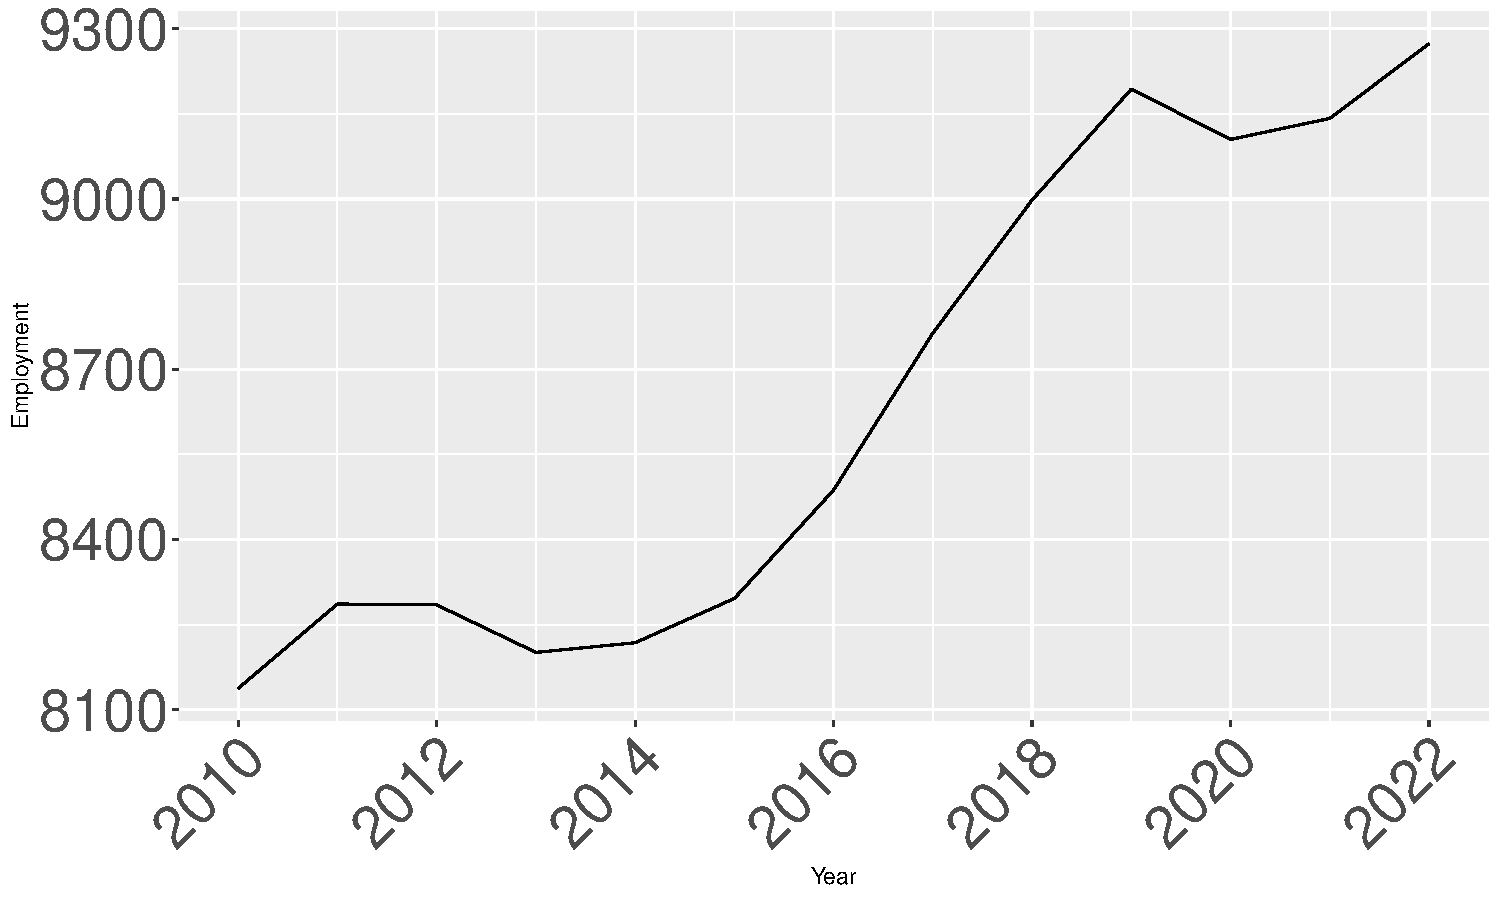
\includegraphics[width=\textwidth]{imgs/employment.pdf}
		\caption{The employment ratio}
		\label{fig:employment}
	\end{minipage}
\end{figure}

It is interesting to compare how suicides increased for all the ranges of age available to 
guess which categories were affected the most (\ref{fig:pl-fat-19_85-12_13}, \ref{fig:pl-fat-19_85-13_14}),
in actuality the relative change in suicides for different ranges of years is not guaranteed 
to be influenced by the employment ratio.
It is also interesting to see how people working in different areas committed suicide during the years
to look for correlations with the employment ratio (\ref{fig:pl-fat-job-1999}).
%
%The following graphs report the trend of the average income, the trend of the employment, 
%the trend of suicides committed by people aged between 30 and 50,
%the trend of fatal suicides committed by people among
%the age between 19 and 34 (more likely to commit suicide because of unemployment) and the trend of fatal
%suicides divided by their job.
%

\begin{figure}[H]
	\centering
	\begin{minipage}{0.45\textwidth}
		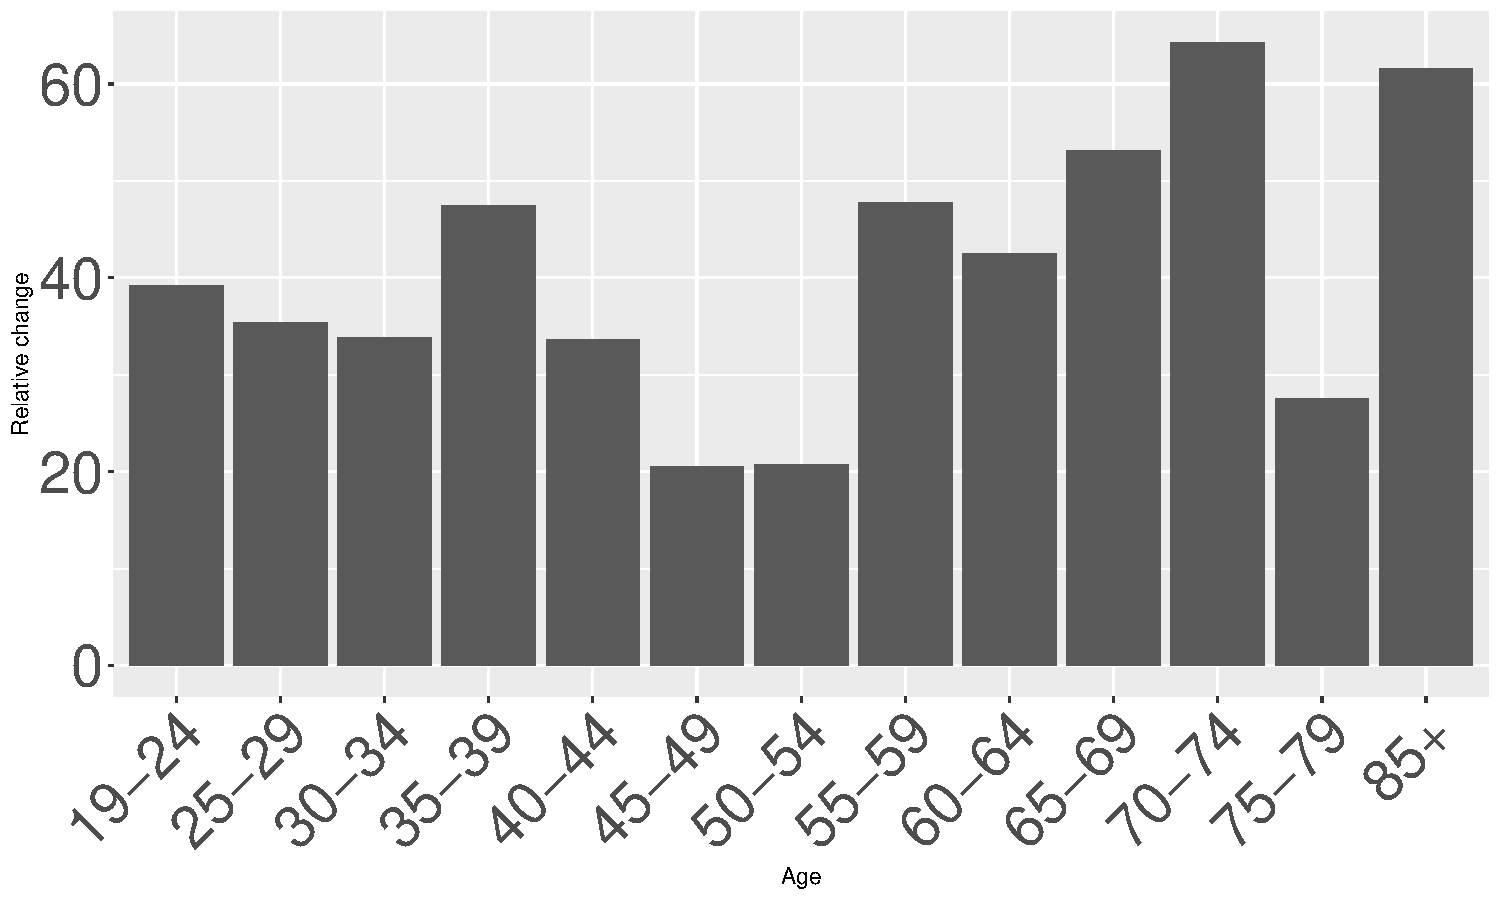
\includegraphics[width=\textwidth]{imgs/pl-fat-19_85-12_13.pdf}
		\caption{Relative change in fatal suicides from 2012 to 2013}
		\label{fig:pl-fat-19_85-12_13}
	\end{minipage}
	\hfill
	\begin{minipage}{0.45\textwidth}
		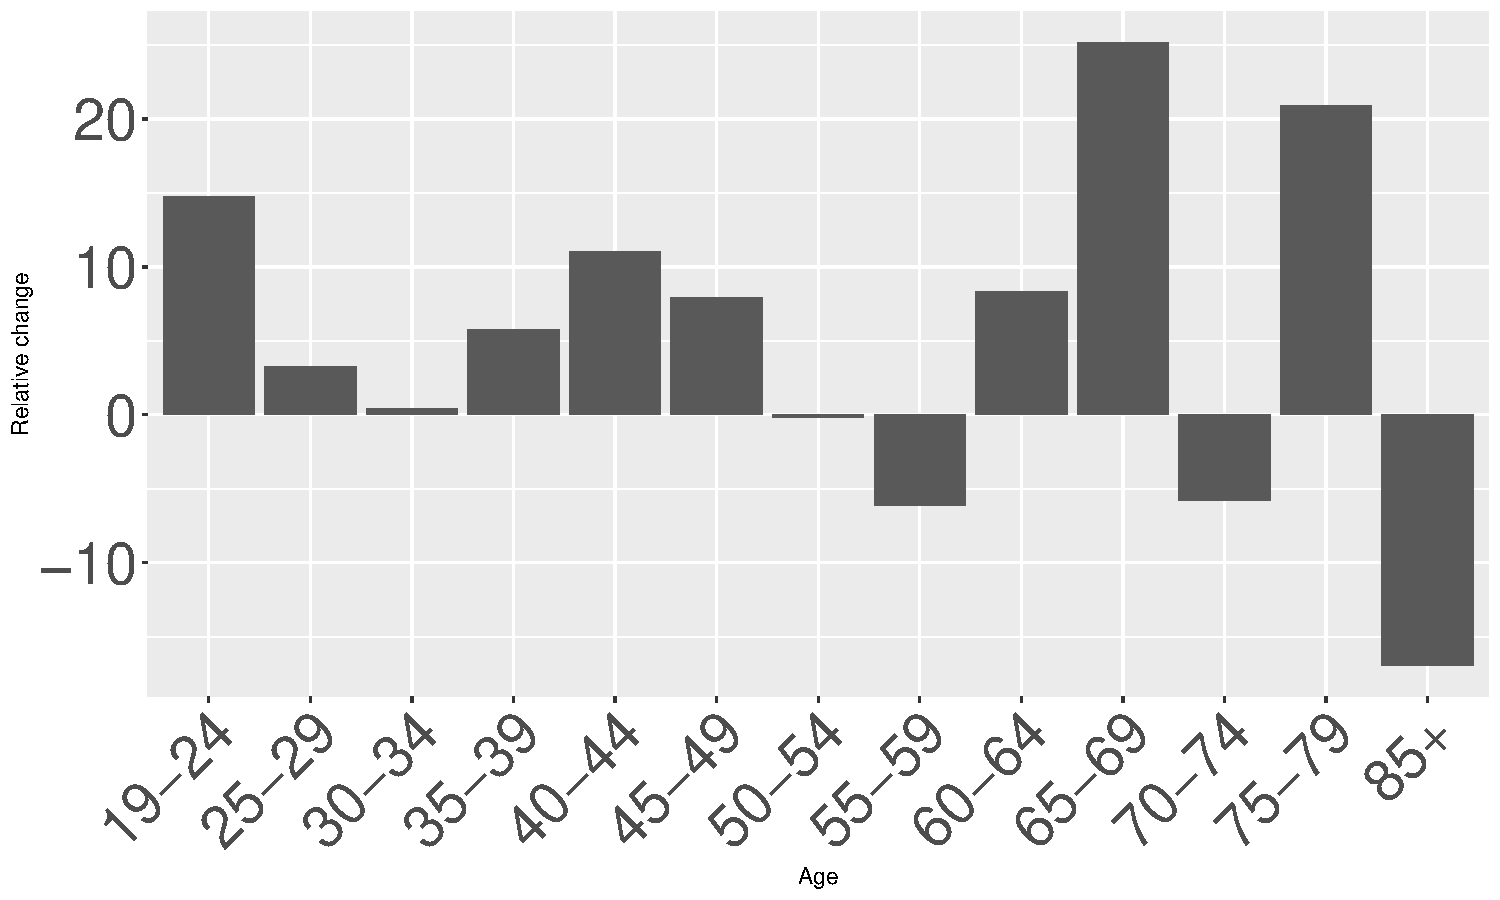
\includegraphics[width=\textwidth]{imgs/pl-fat-19_85-13_14.pdf}
		\caption{Relative change in fatal suicides from 2013 to 2014}
		\label{fig:pl-fat-19_85-13_14}
	\end{minipage}
\end{figure}

\begin{figure}[H]
	\centering
	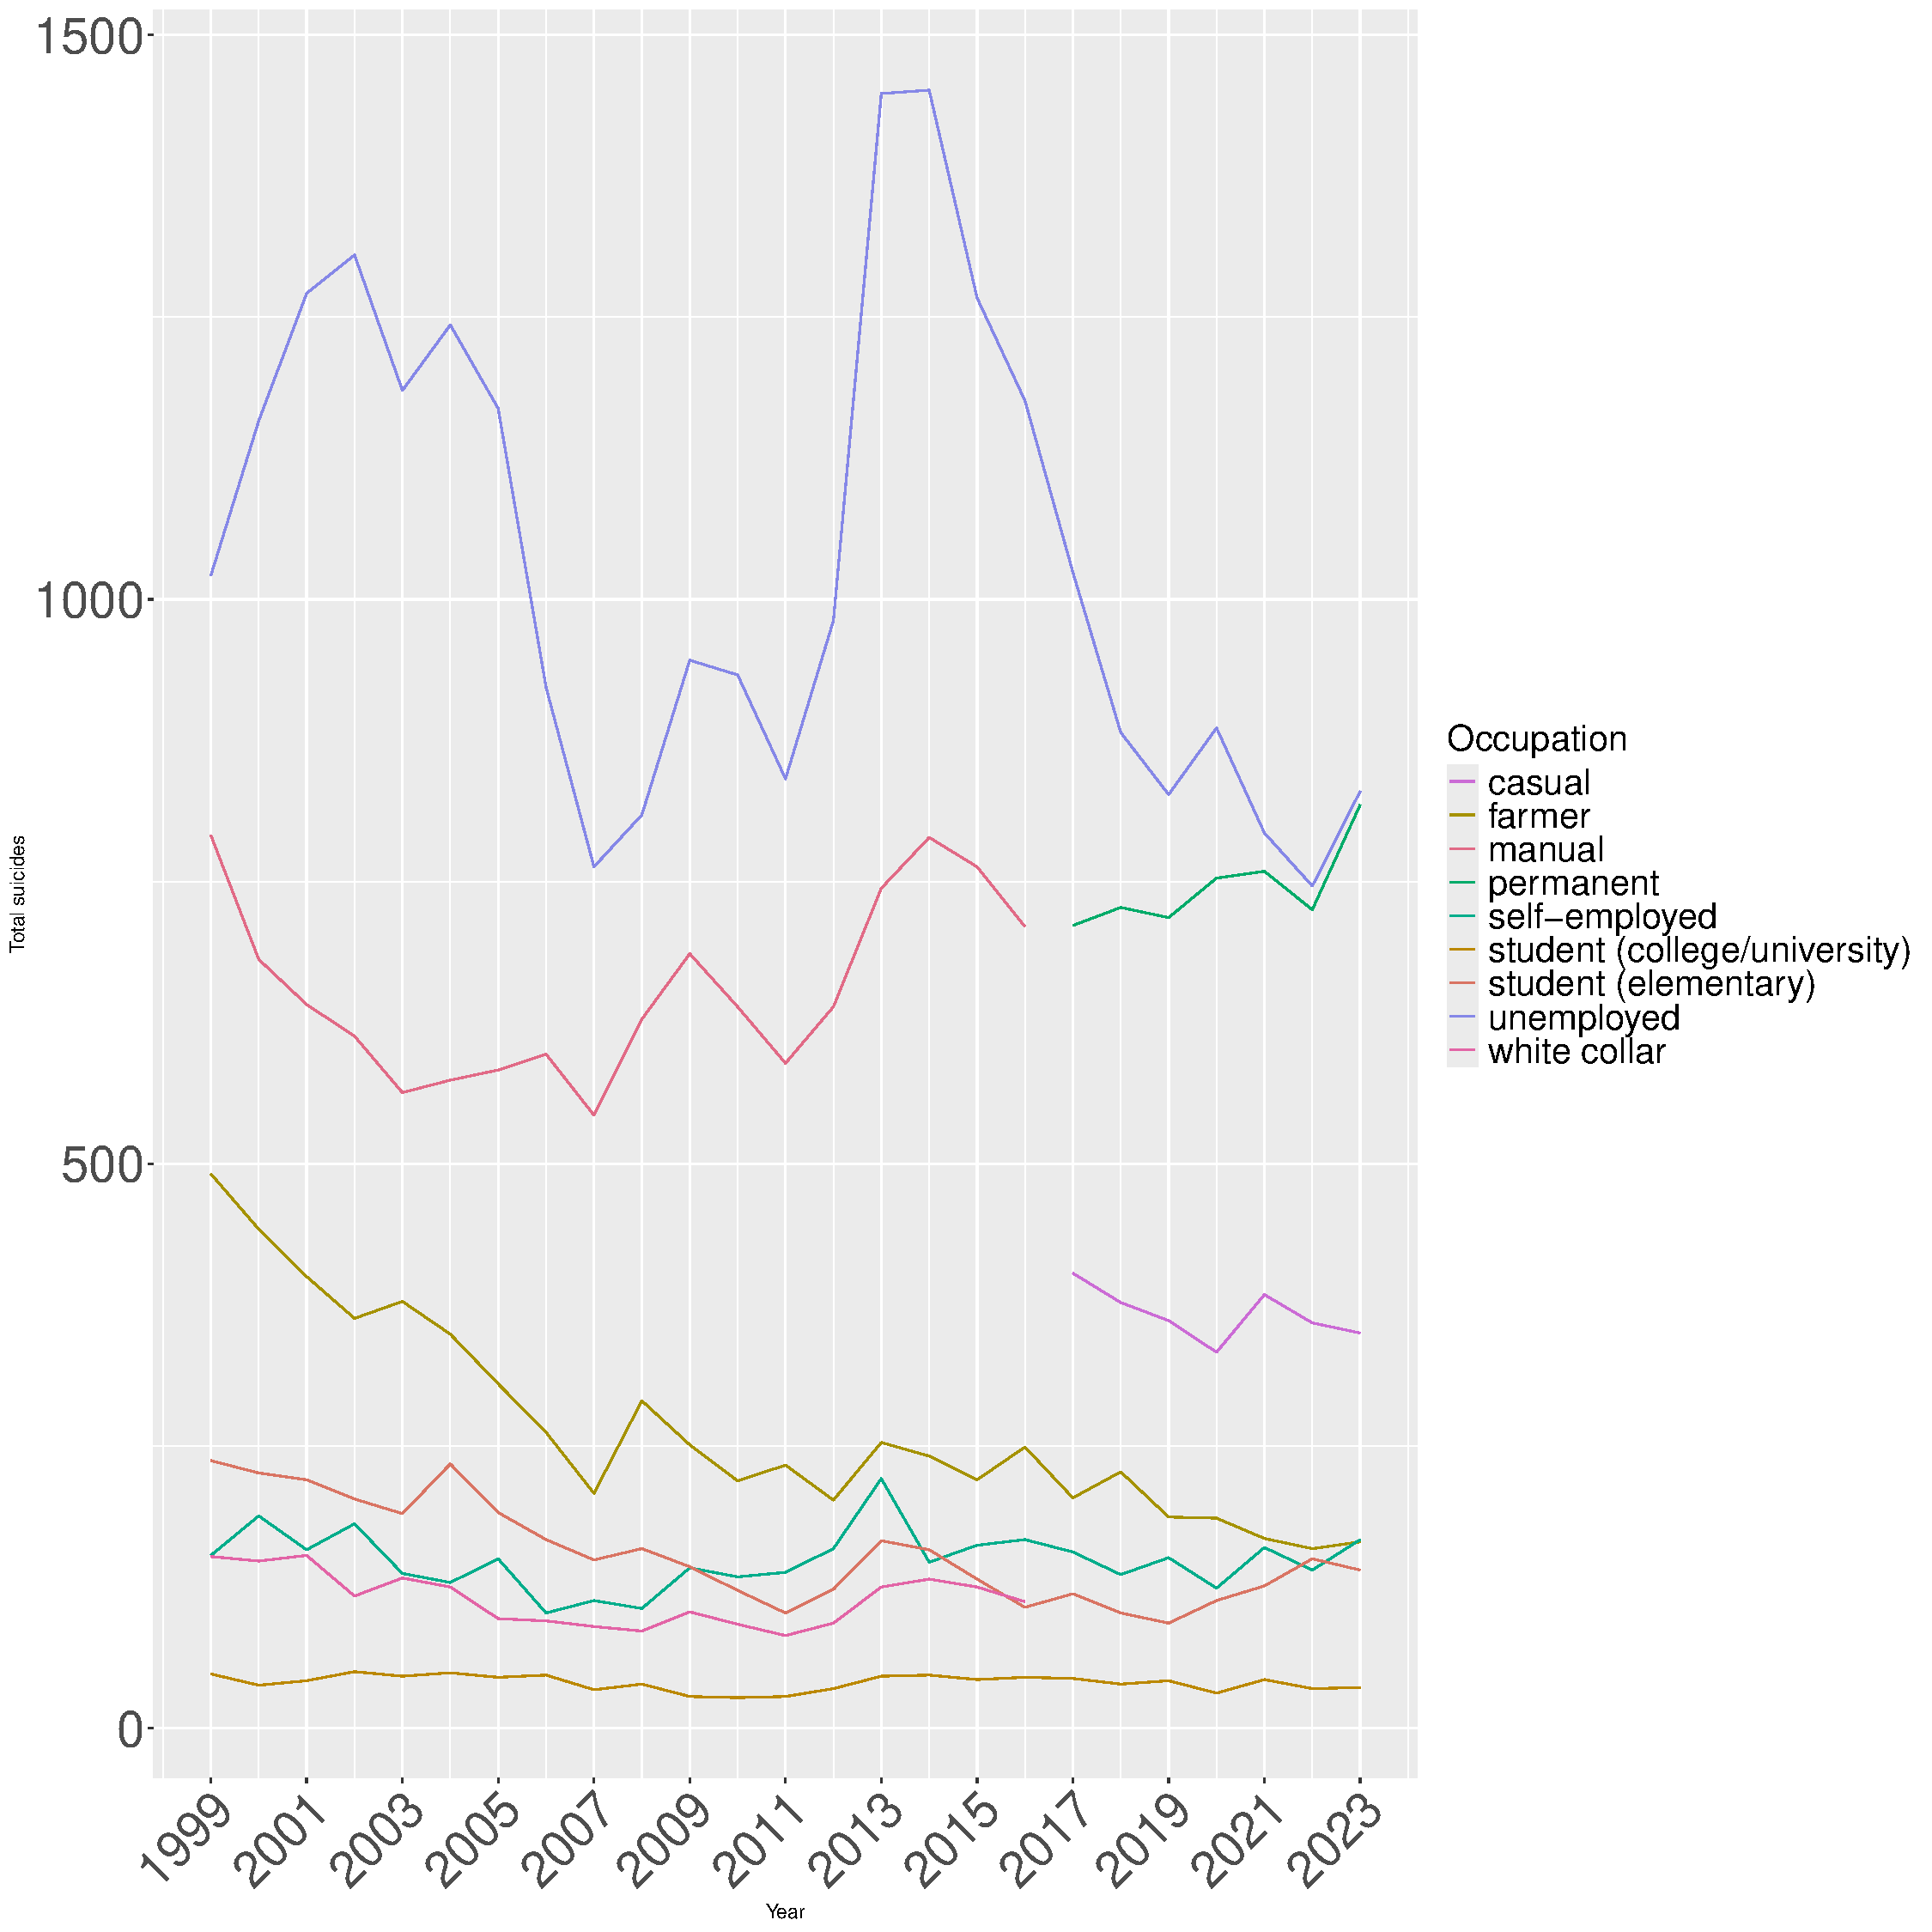
\includegraphics[width=0.65\textwidth]{imgs/pl-fat-job-1999.pdf}
	\caption{Fatal suicides of people with different jobs}
	\label{fig:pl-fat-job-1999}
\end{figure}
%
\hfill \\
%
The employment ratio decreased between 2012 and 2013 and, in the same period,
unemployed people in particular committed more suicides, then again between 2019 and 2020 
the employment ratio decreased and suicides among unemployed people increased.
%
It is worth noticing that, when it comes to age groups, none of them showed a decrease between 
2012 and 2013, this suggesting either that unemployed people cover the whole spectrum of ages
or that the correlation between the decrease of employment ratio and the increment in suicides by
unemployed people is not so strong.
Between 2013 and 2014 the situation generally improved. \\
Between 2019 and 2020 another decrease in the employment ratio took place but, in this
case, the increase in the number of suicides was not as significant as the one between 2012 and 2013
(\ref{fig:pl-fat-19_85-19_20}),
moreover, only a few age groups showed an increase in the number of suicides. 
Between 2020 and 2021, when the employment ratio increased, there was no significant improvement,
on the contrary, the number of people aged between 45 and 49, between 55 and 59 and between 70 and 74
that attempted suicide
increased (\ref{fig:pl-fat-19_85-20_21}) whereas it decreased between 2019 and 2020.
The enormous increase in the number of suicides between 2012 and 2013 is likely to be the consequence 
of a more complex phenomenon rather than just the decrease in the employment ratio.
%
%
\begin{figure}[H]
	\begin{minipage}{0.45\textwidth}
		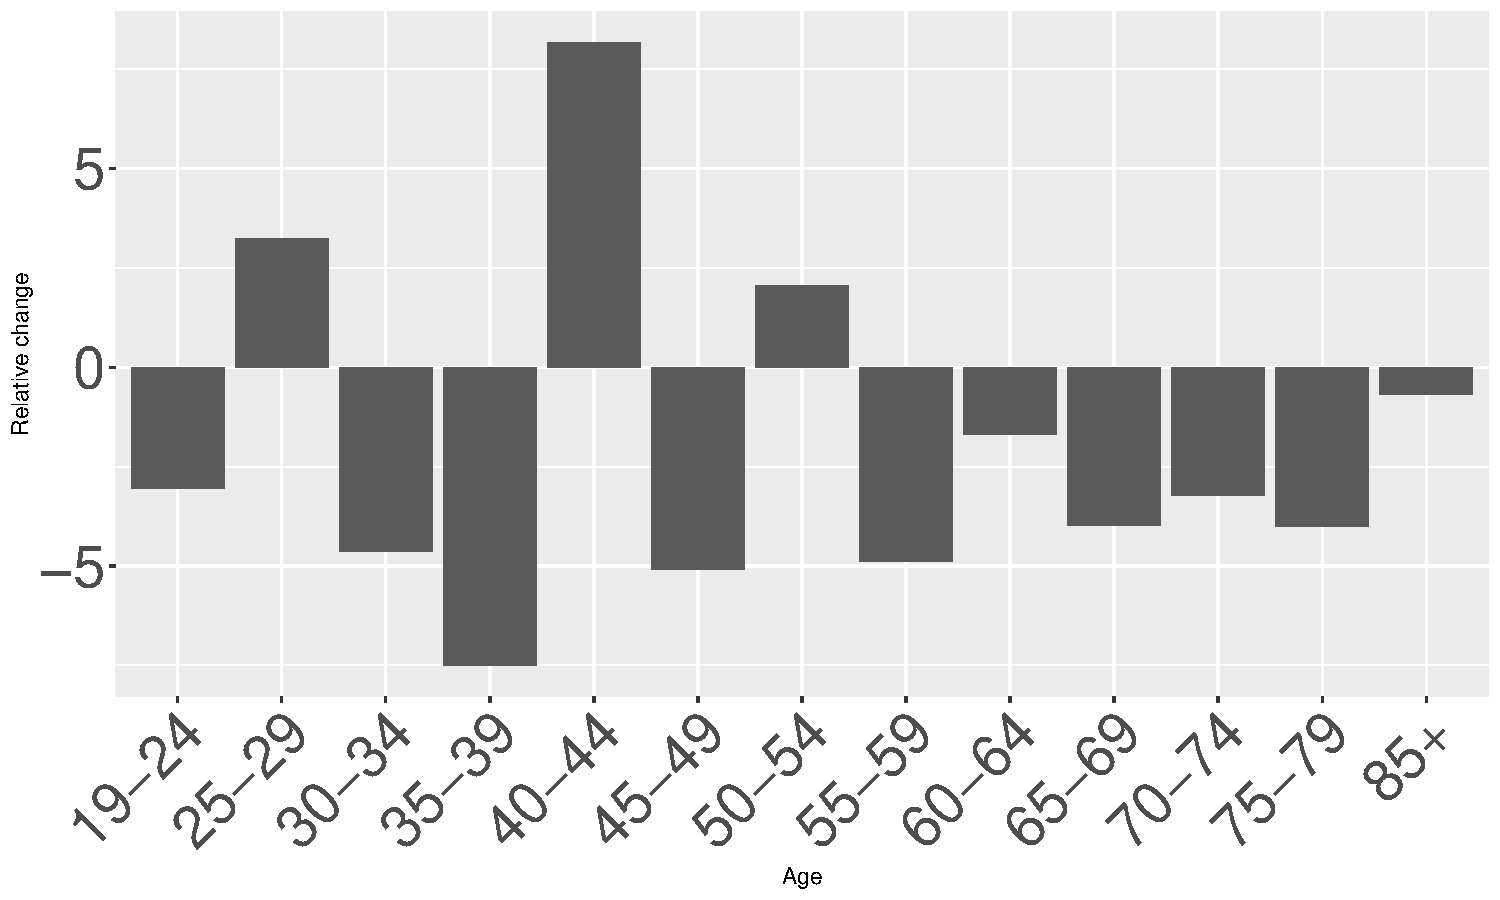
\includegraphics[width=\textwidth]{imgs/pl-fat-19_85-19_20.pdf}
		\caption{Relative change in fatal suicides from 2019 to 2020}
		\label{fig:pl-fat-19_85-19_20}
	\end{minipage}
	\hfill
	\begin{minipage}{0.45\textwidth}
		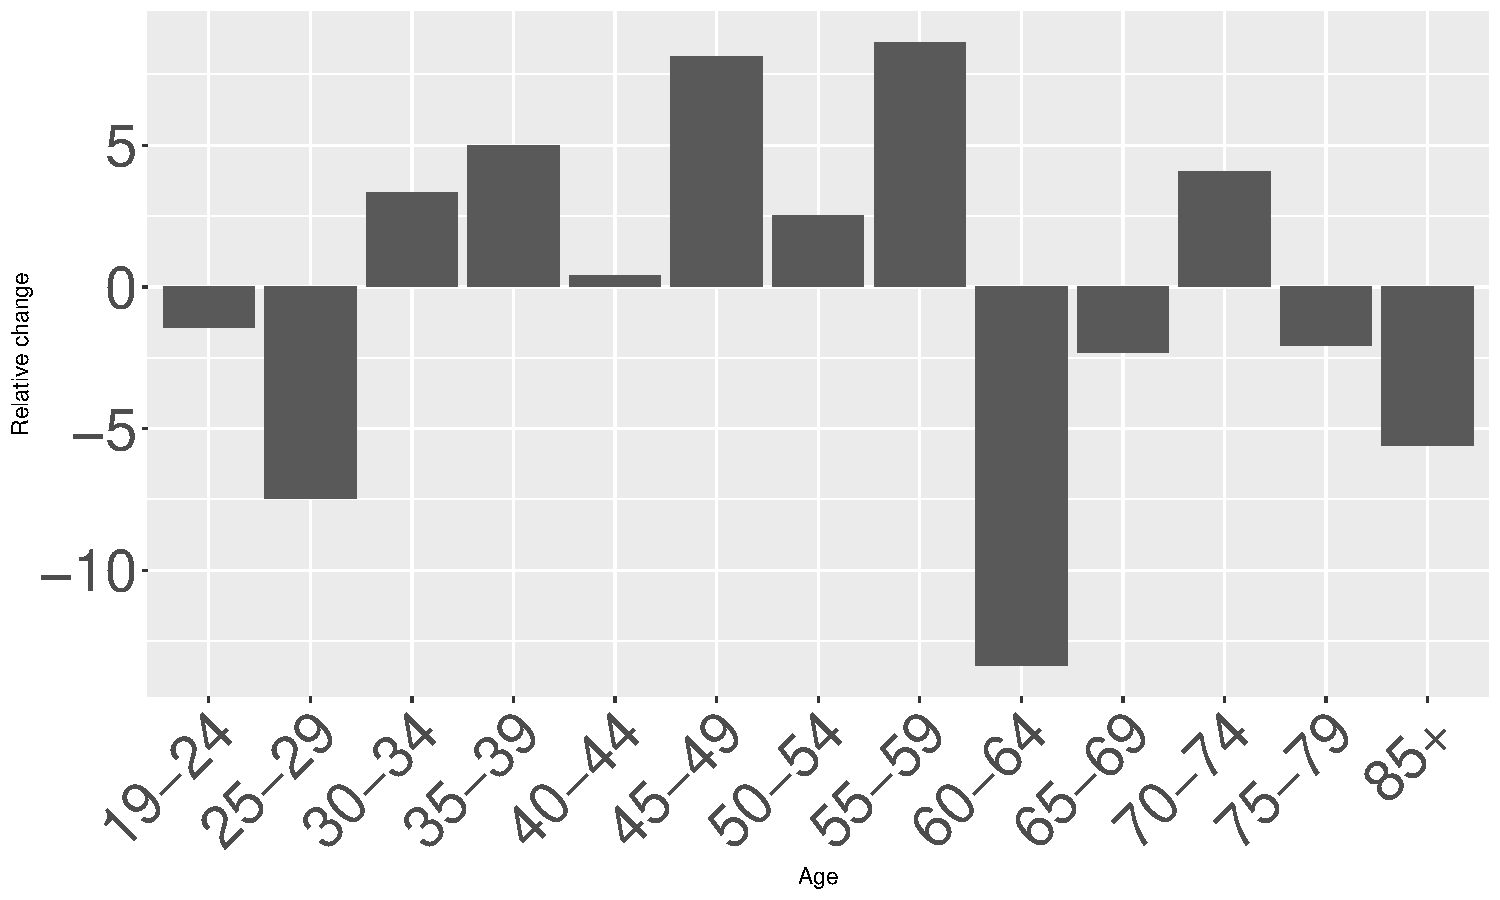
\includegraphics[width=\textwidth]{imgs/pl-fat-19_85-20_21.pdf}
		\caption{Relative change in fatal suicides from 2020 to 2021}
		\label{fig:pl-fat-19_85-20_21}
	\end{minipage}
\end{figure}
%
%
%
% On the other hand, when focusing on people among the age between 19 and 34, although the 
% number of suicides increases a lot between 2012 and 2013, no significant increase happens between 2019 and 
% 2020, moreover, the number of total suicides (displayed in the first graph) between 2019 and 2020 decreased,
% this suggests that either the decrease of the employment ratio during 2019 and 2020 was less impactful
% or that the decrease of the employment ratio between 2012 and 2013 was part of a more complex phenomenon. \\
% It is still worth noting that between 2012 and 2013 most suicides were committed by people aged between 50 and 59,
% then people in that range of age slowly decreased the number of suicides while younger people increased them:
% 
% 
%I would say that people aged between 50 and 59 would be more likely to commit suicide due to an
%economic crisis. What surprises is that the increase between 2012 and 2013 was even worse than that between
%2007 and 2008, the period of the great financial crisis.
%
%
%
%
%\section{Suicides in different cities}
%The data are made available by garrisons (garnizon) of different cities,
%at first glance Katowice displays a worrying predominance in the total number
%of suicides. 
%
%\begin{figure}[H]
%	\centering
%	\begin{minipage}{0.65\textwidth}
%		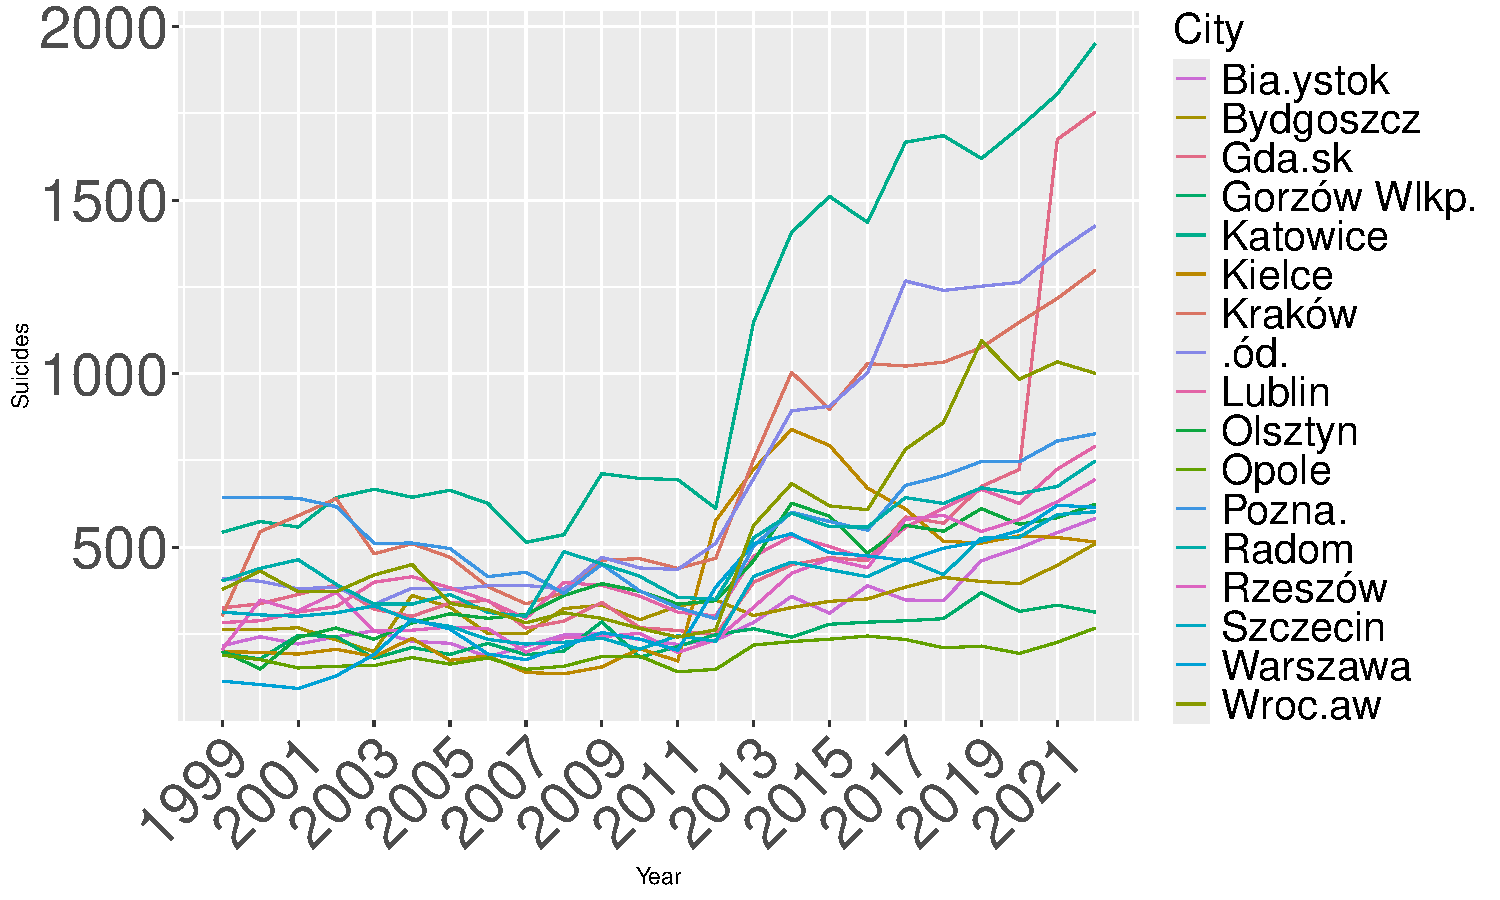
\includegraphics[width=\textwidth]{imgs/city_attempted.pdf}
%		\caption{Attempted suicides in different cities}
%	\end{minipage}
%	\hfill
%	\begin{minipage}{0.65\textwidth}
%		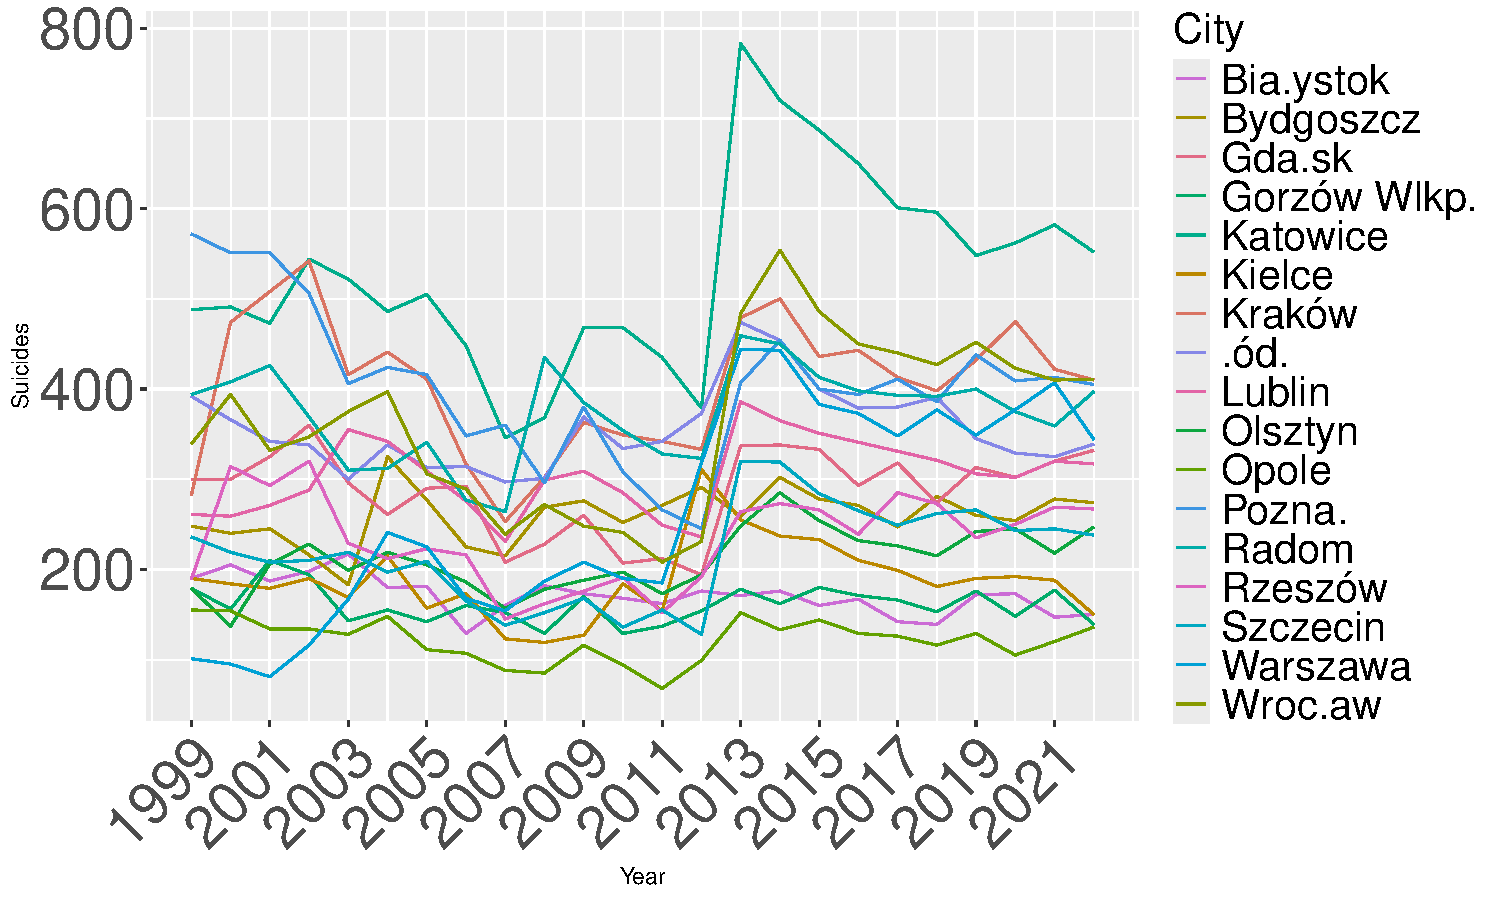
\includegraphics[width=\textwidth]{imgs/city_fatal.pdf}
%		\caption{Fatal suicides in different cities}
%	\end{minipage}
%\end{figure}
%
%
% new page

%
%
\section{Focus on the single variables}
%
\subsection{City}
Figures \ref{fig:city_att}, \ref{fig:city_fat}, \ref{fig:city_foa}
show that in 2022 the city with the highest rate of suicide attempts per population
was Katowice (645 attempts every 100000 people), followed by Rzeszów (377 attempts every 100000 people),
Olsztyn (359 attempts every 100000 people), Radom (350 attempts every 100000 people)
and Gdańsk (301 attempts every 100000 people).
The cities with the lowest rate of suicide attempts per population were Warszawa
(34 every 100000), Bydgoszcz (144 every 100000), Szczecin (149 every 100000) 
The city with the highest rate of fatal suicide attempts per population
was Radom (186 every 100000), followed by Katowice (183 every 100000),  
Rzeszów (145 every 100000) and Olsztyn (142 every 100000).
The cities with the lowest rate of fatal suicide attempts per population are 
Warszawa (19 every 100000), Białystok (51 every 100000), Kraków (53 every 100000).
In Poland (36.82 milion of inhabitants), during 2022, 14520 suicide attempts were
registered (39 every 100000) of which 5108 resulted in death (14 every 100000),
the reason why densities of suicides per inhabitants result higher when considering
the single city is probably because the considered population is only relative
to the city whereas the registered cases of suicide attempts in the garrisons
are comprehensive of a larger area than just the city each garrison refers to.
\begin{figure}[H]
	\centering
		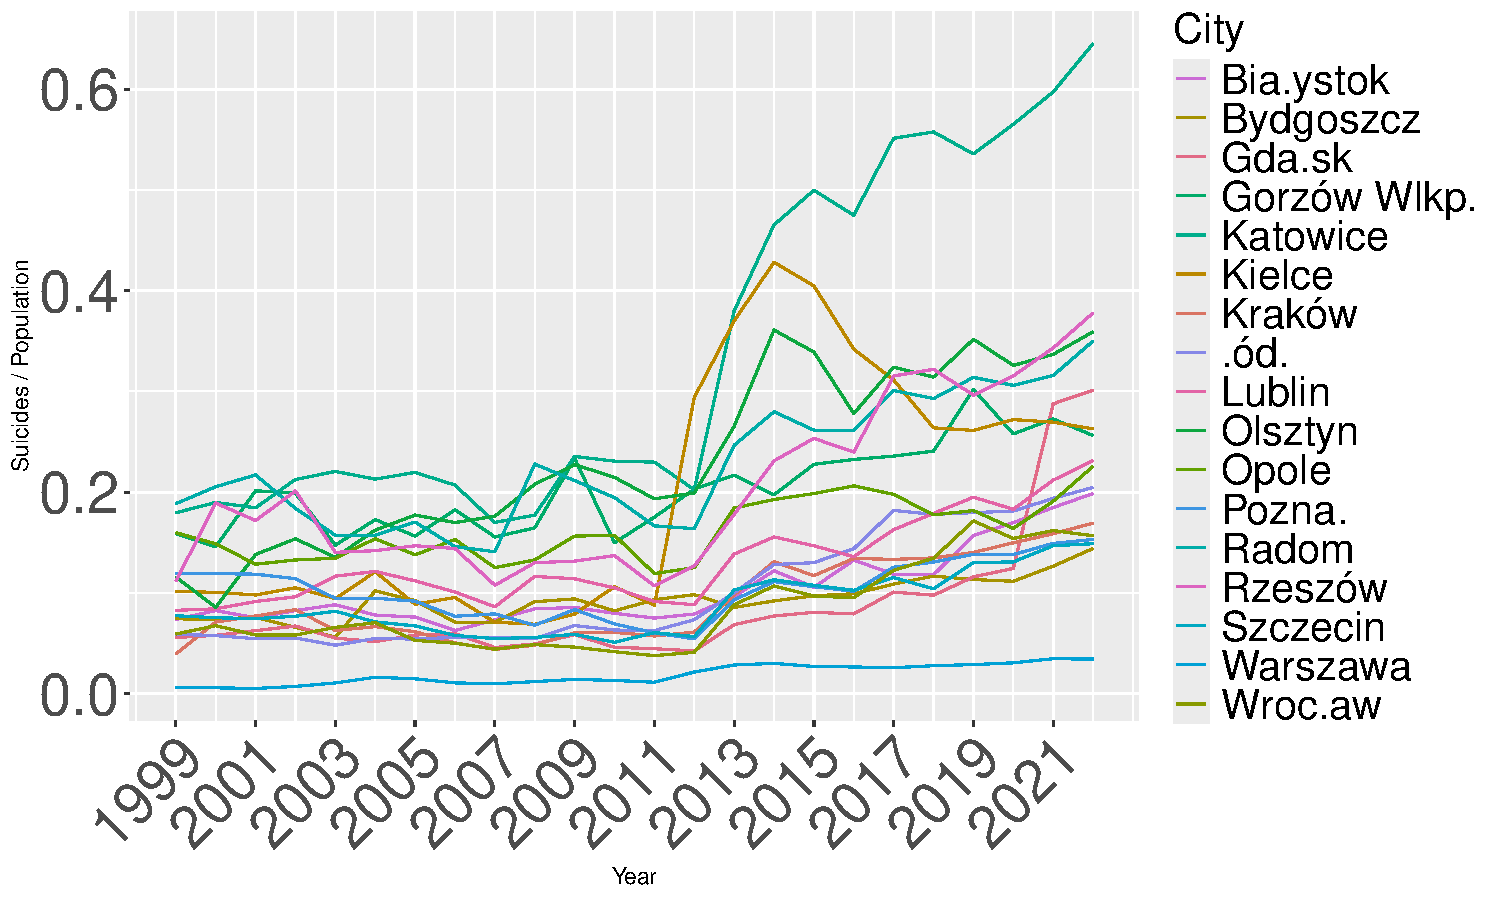
\includegraphics[width=0.65\textwidth]{imgs/city_att.pdf}
		\caption{Suicide attempts in different cities from 1999 to 2022}
		\label{fig:city_att}
\end{figure}

\begin{figure}[H]
	\centering
		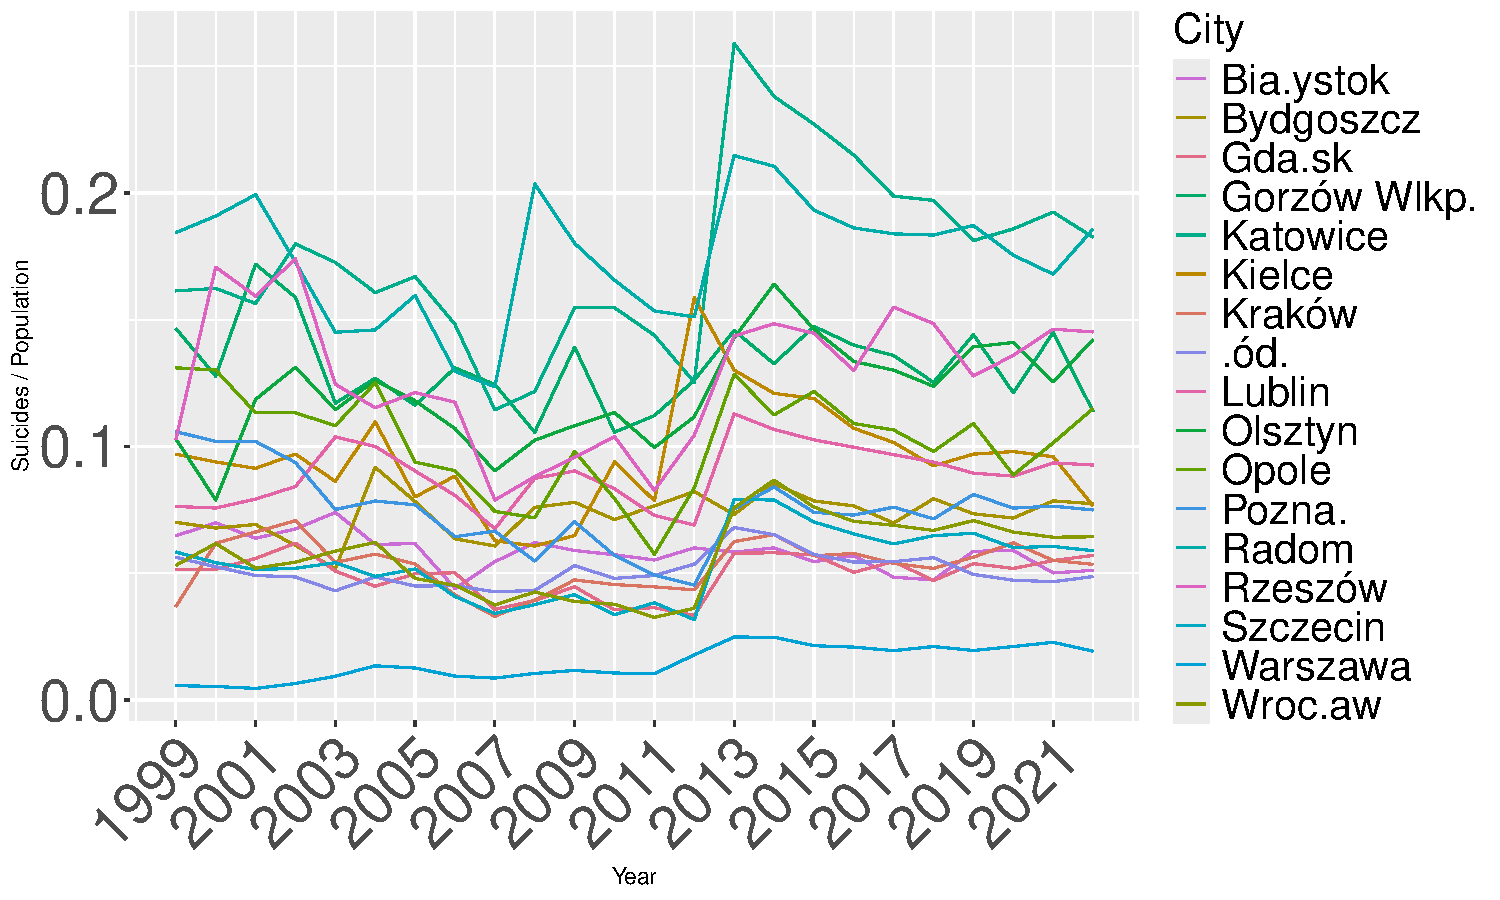
\includegraphics[width=0.65\textwidth]{imgs/city_fat.pdf}
		\caption{Suicide attempts in different cities from 1999 to 2022}
		\label{fig:city_fat}
\end{figure}

\begin{figure}[H]
	\centering
		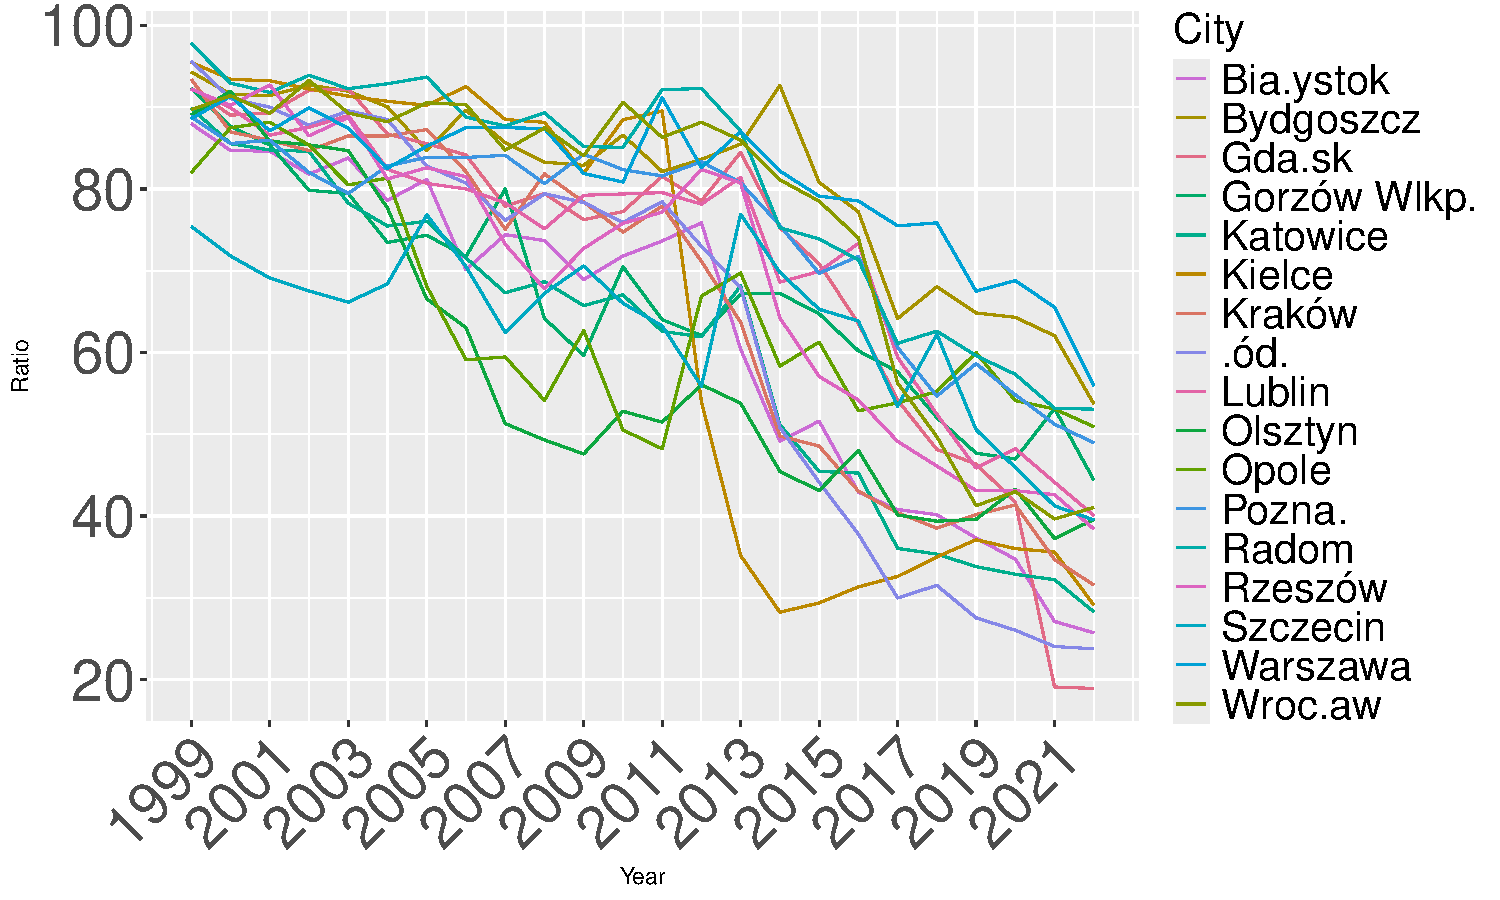
\includegraphics[width=0.65\textwidth]{imgs/city_foa.pdf}
		\caption{Fatal suicide attempts over all attempts in different cities from 1999 to 2022}
		\label{fig:city_foa}
\end{figure}




\subsection{Age}
%Analysis on age.
As shown in figures \ref{fig:age_attempted}, 
\ref{fig:age_fatal}, \ref{fig:age_foa},
the ranges of age that show the most worrying increment in attempted suicides 
are the youngest ones, whereas the oldest ones keep a slightly increasing trend and 
appear to be less affected by the economic crisis.
People aged over 40 and under 70 are the ones to commit the most fatal suicides and are those
who show the most significant increment between 2012 and 2013.
Older people are the most likely to unfortunately succeed in their attempt and younger people
are the least likely to do so, the difference in this ratio of fatal over attempted suicides 
increased in time.
%
\begin{figure}[H]
    \centering
    \begin{minipage}{0.65\textwidth}
        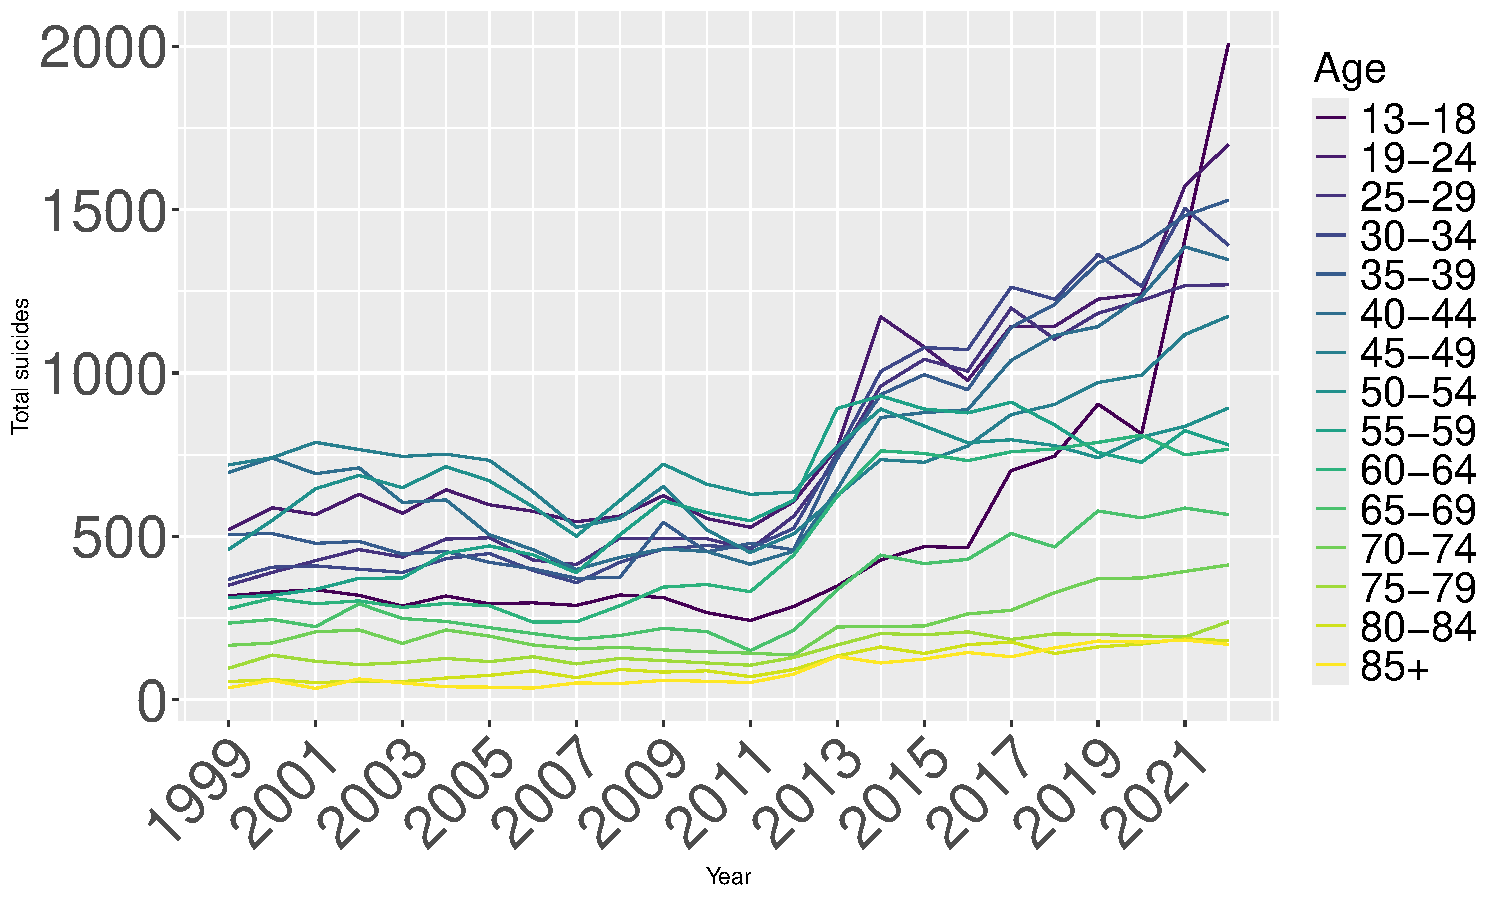
\includegraphics[width=\textwidth]{imgs/age_attempted.pdf}
        \caption{Trend of attempted suicides by age range}
	%label for reference 
	\label{fig:age_attempted}
    \end{minipage}
    \hfill
    \begin{minipage}{0.65\textwidth}
        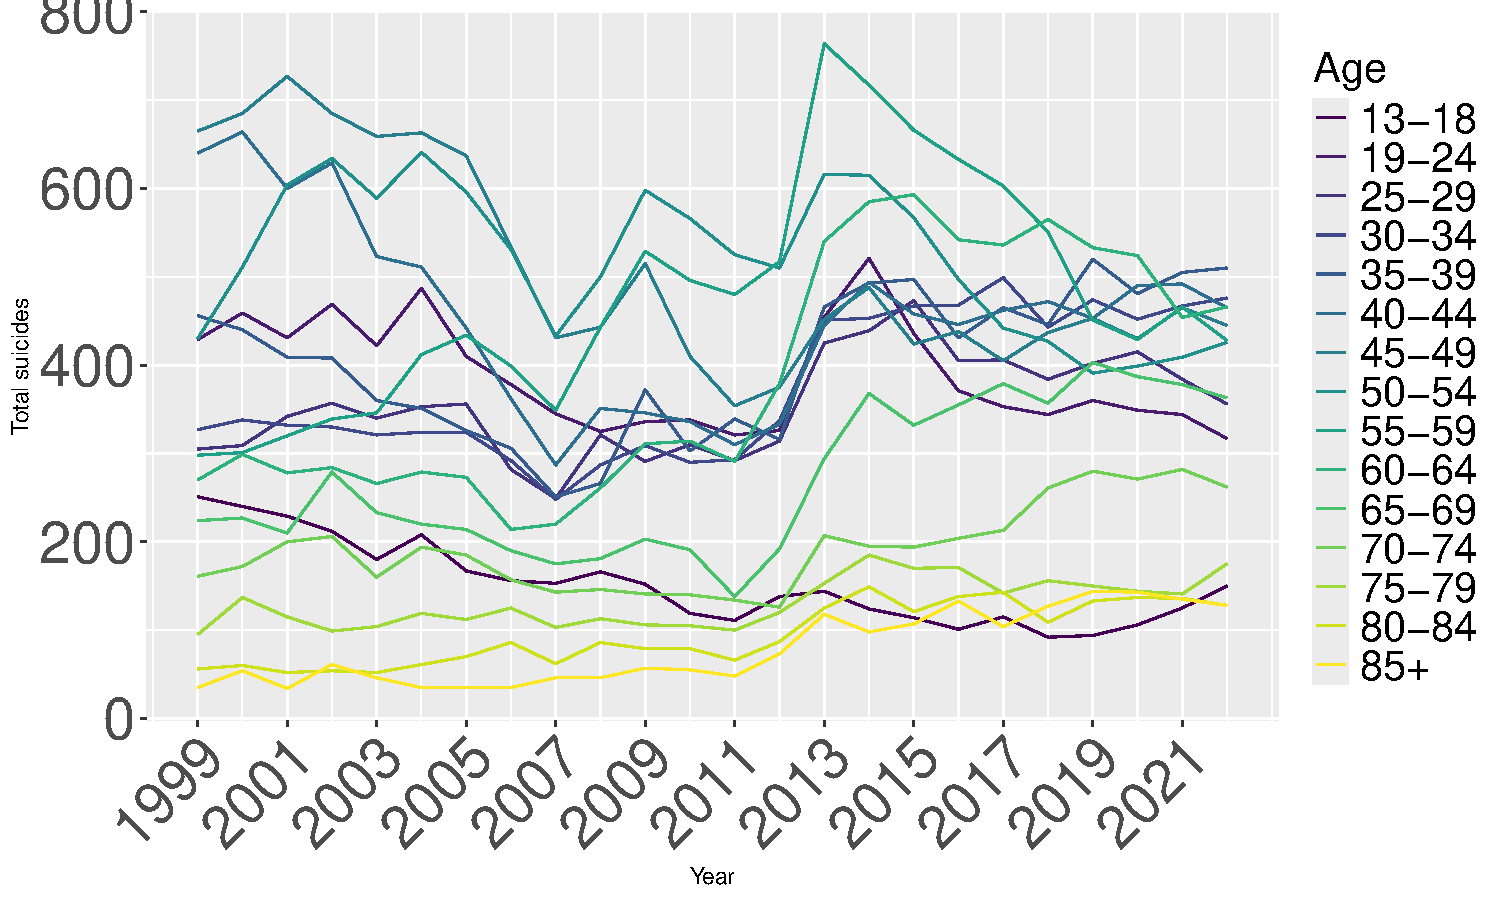
\includegraphics[width=\textwidth]{imgs/age_fatal.pdf}
        \caption{Trend of fatal suicides by age range}
	\label{fig:age_fatal}
    \end{minipage}
\end{figure}

\begin{figure}[H]
    \centering
    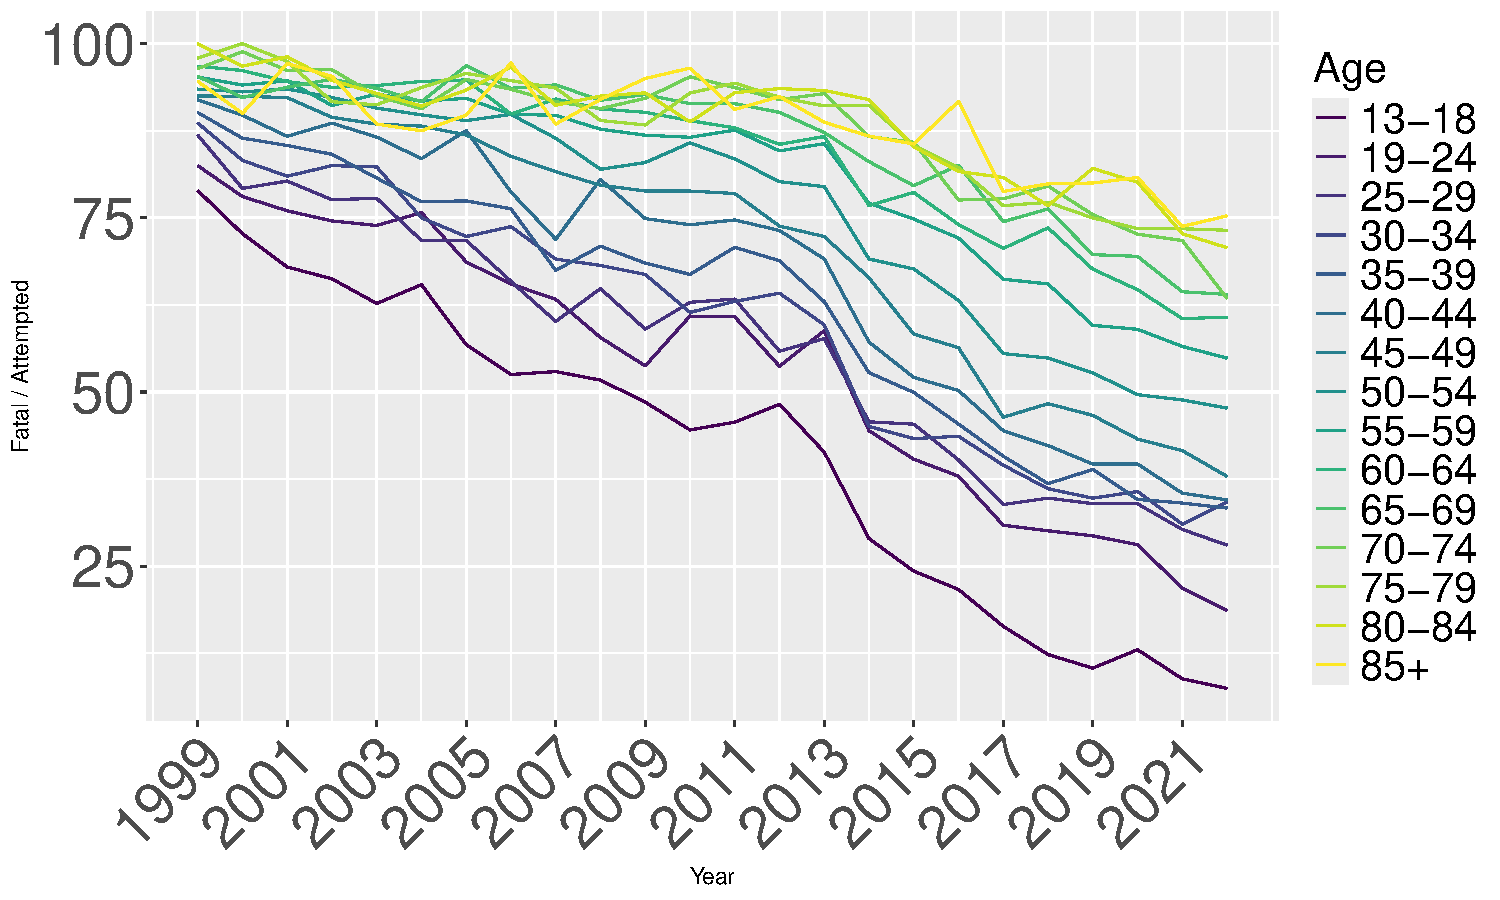
\includegraphics[width=0.65\textwidth]{imgs/age_foa.pdf}
    \caption{Trend of fatal over attempted suicides by age range}
    \label{fig:age_foa}
\end{figure}
%
The heatmap in figure \ref{fig:age_foa_heat} confirms that for younger people the ratio of fatal over 
attempted suicides improved (decreased) in time more than it happened for older people.
Figure \ref{fig:age_city_att_op-991020} shows that from 1999 to 2020 there was no significant 
change in how people from different age ranges attempted suicide in different cities,
what is revealed from a first look at the yougest range is that Gdańsk was the city with the
smallest number of teenagers attempting suicide in 1999 and became the one with the most
teenagers attempting suicide in 2020, whereas in 2015 Opole had a lot more younger people
attempting suicide with respect to other cities. 
There seems not to be an apparent trend that might suggest 
whether a city needs more prevention programs than others.
When focusing on more recent years (2021 and 2022), as in figure \ref{fig:age_city_att_op-2122},
apart from noticing again the general increase in the percentages of suicides attempted by
the youngest, it becomes more concerning how again Gdańsk displays
the greatest percentage of the youngest attempting suicide, this disproves
the previous naive conclusion: some serious investigation should be made
about why so many teenagers attempted suicide in Gdańsk.
% 
%
\begin{figure}[H]
    \centering
    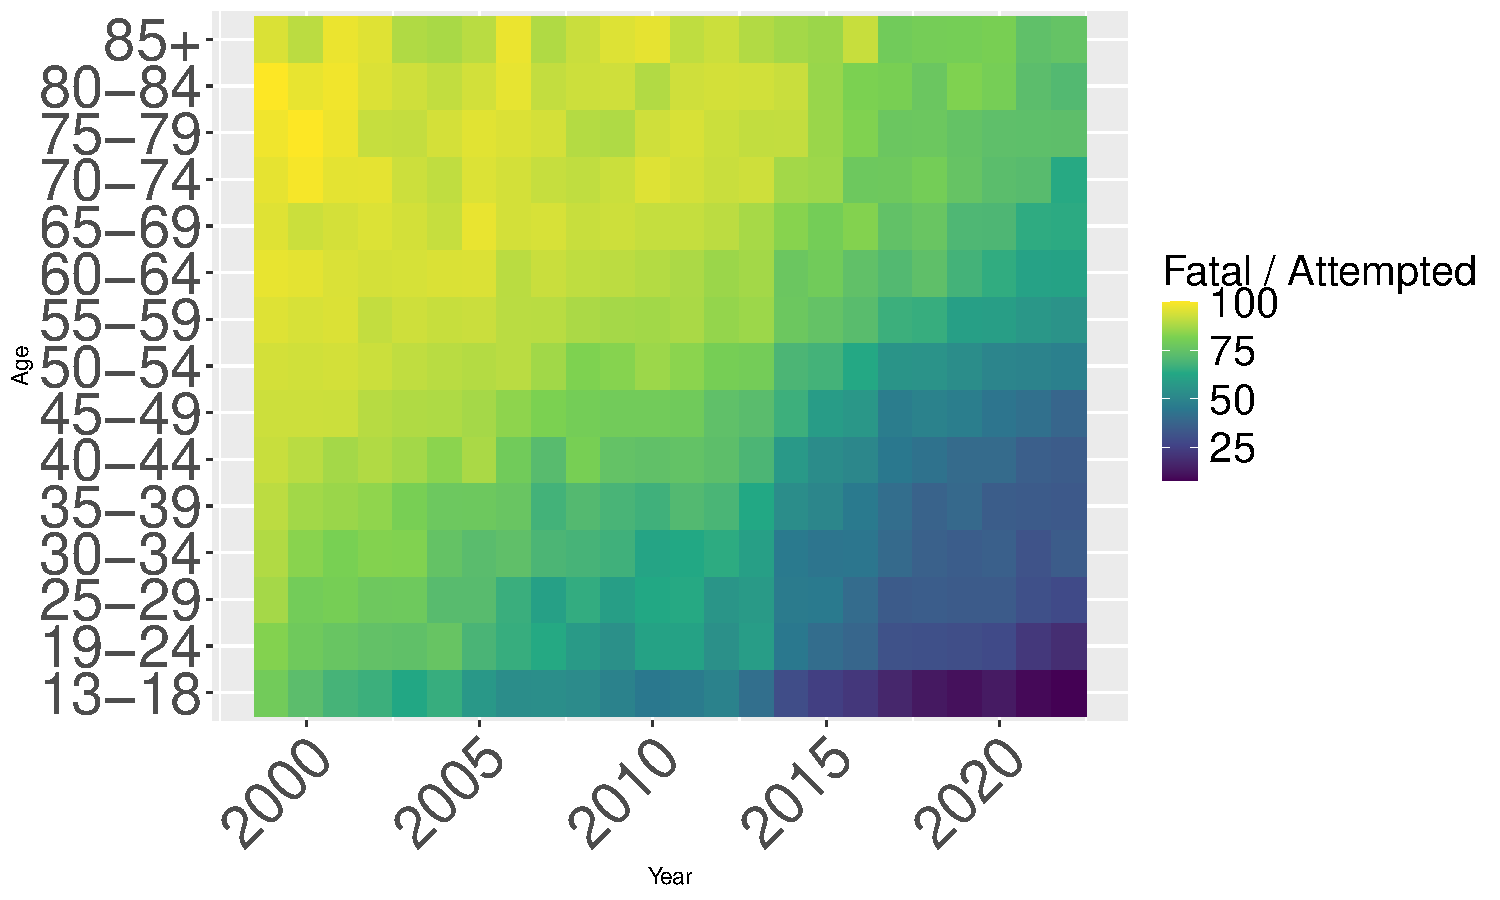
\includegraphics[width=0.65\textwidth]{imgs/age_foa_heat.pdf}
    \caption{Heatmap of fatal over attempted suicides by age range}
    \label{fig:age_foa_heat}
\end{figure}
%
%
%
\begin{figure}[H]
    \centering
    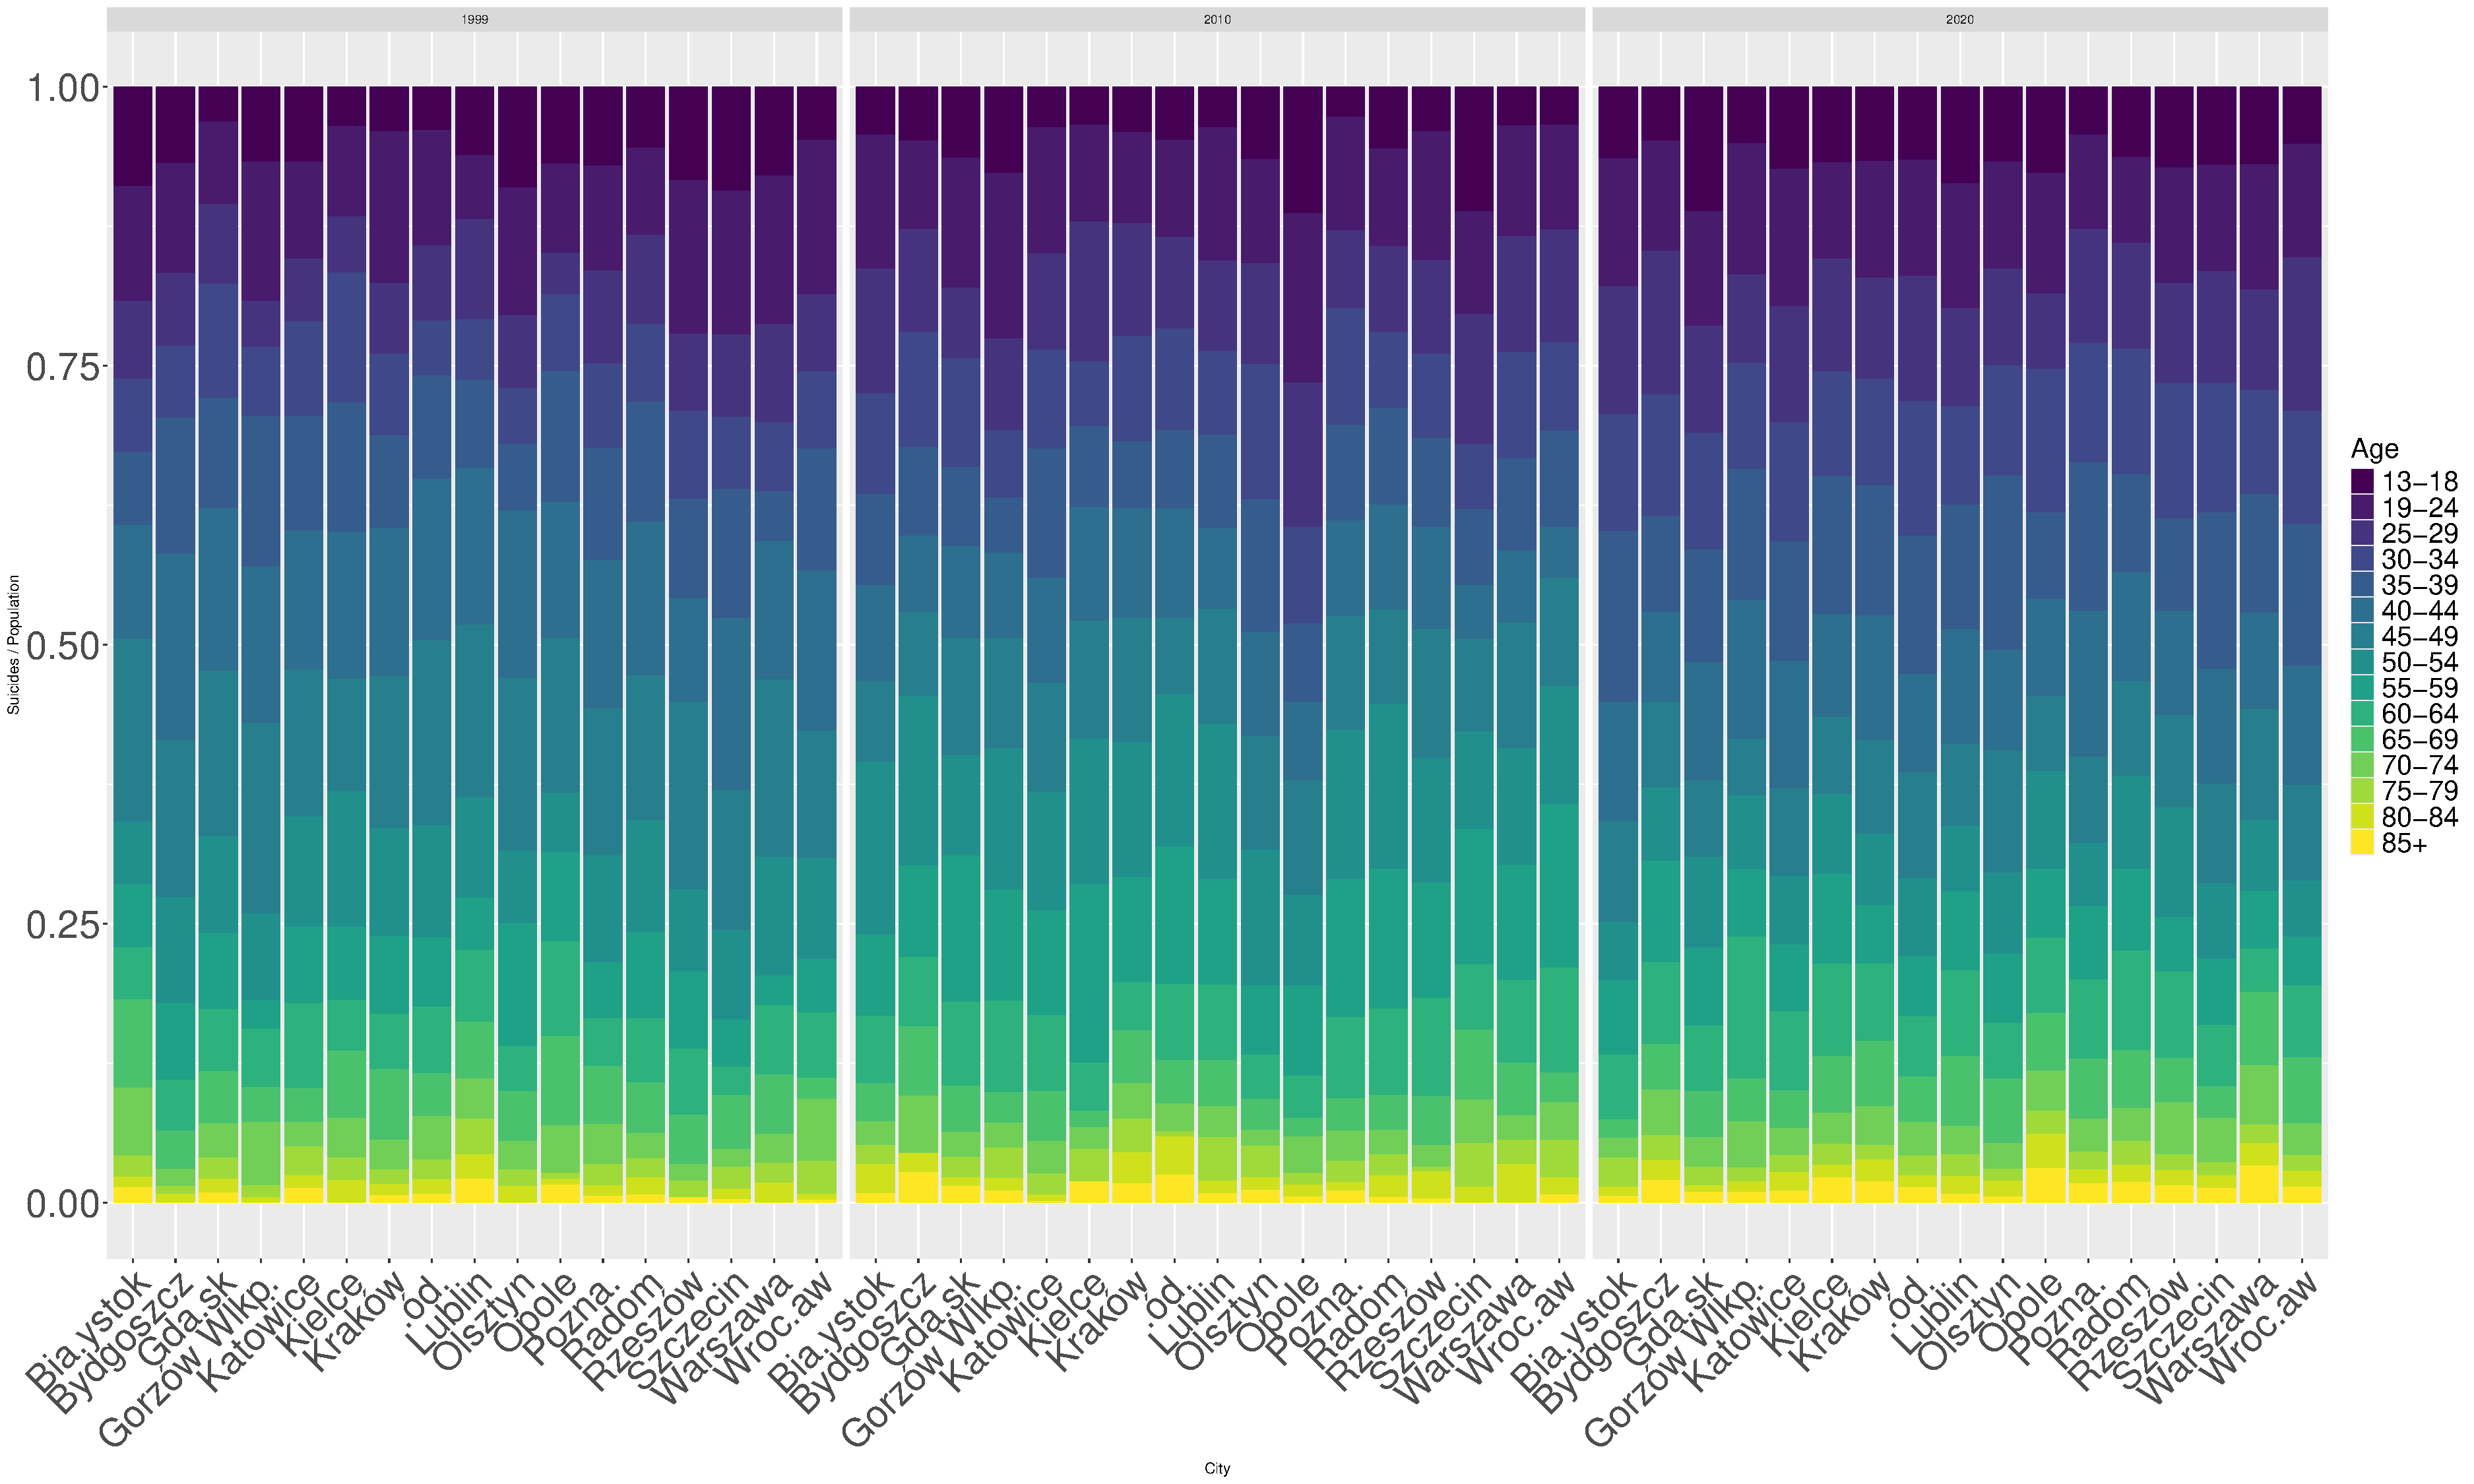
\includegraphics[width=0.65\textwidth]{imgs/age_city_att_op-991020.pdf}
    \caption{Attempted suicides by age range in 1999, 2010 and 2020}
    \label{fig:age_city_att_op-991020}
\end{figure}

\begin{figure}[H]
    \centering
    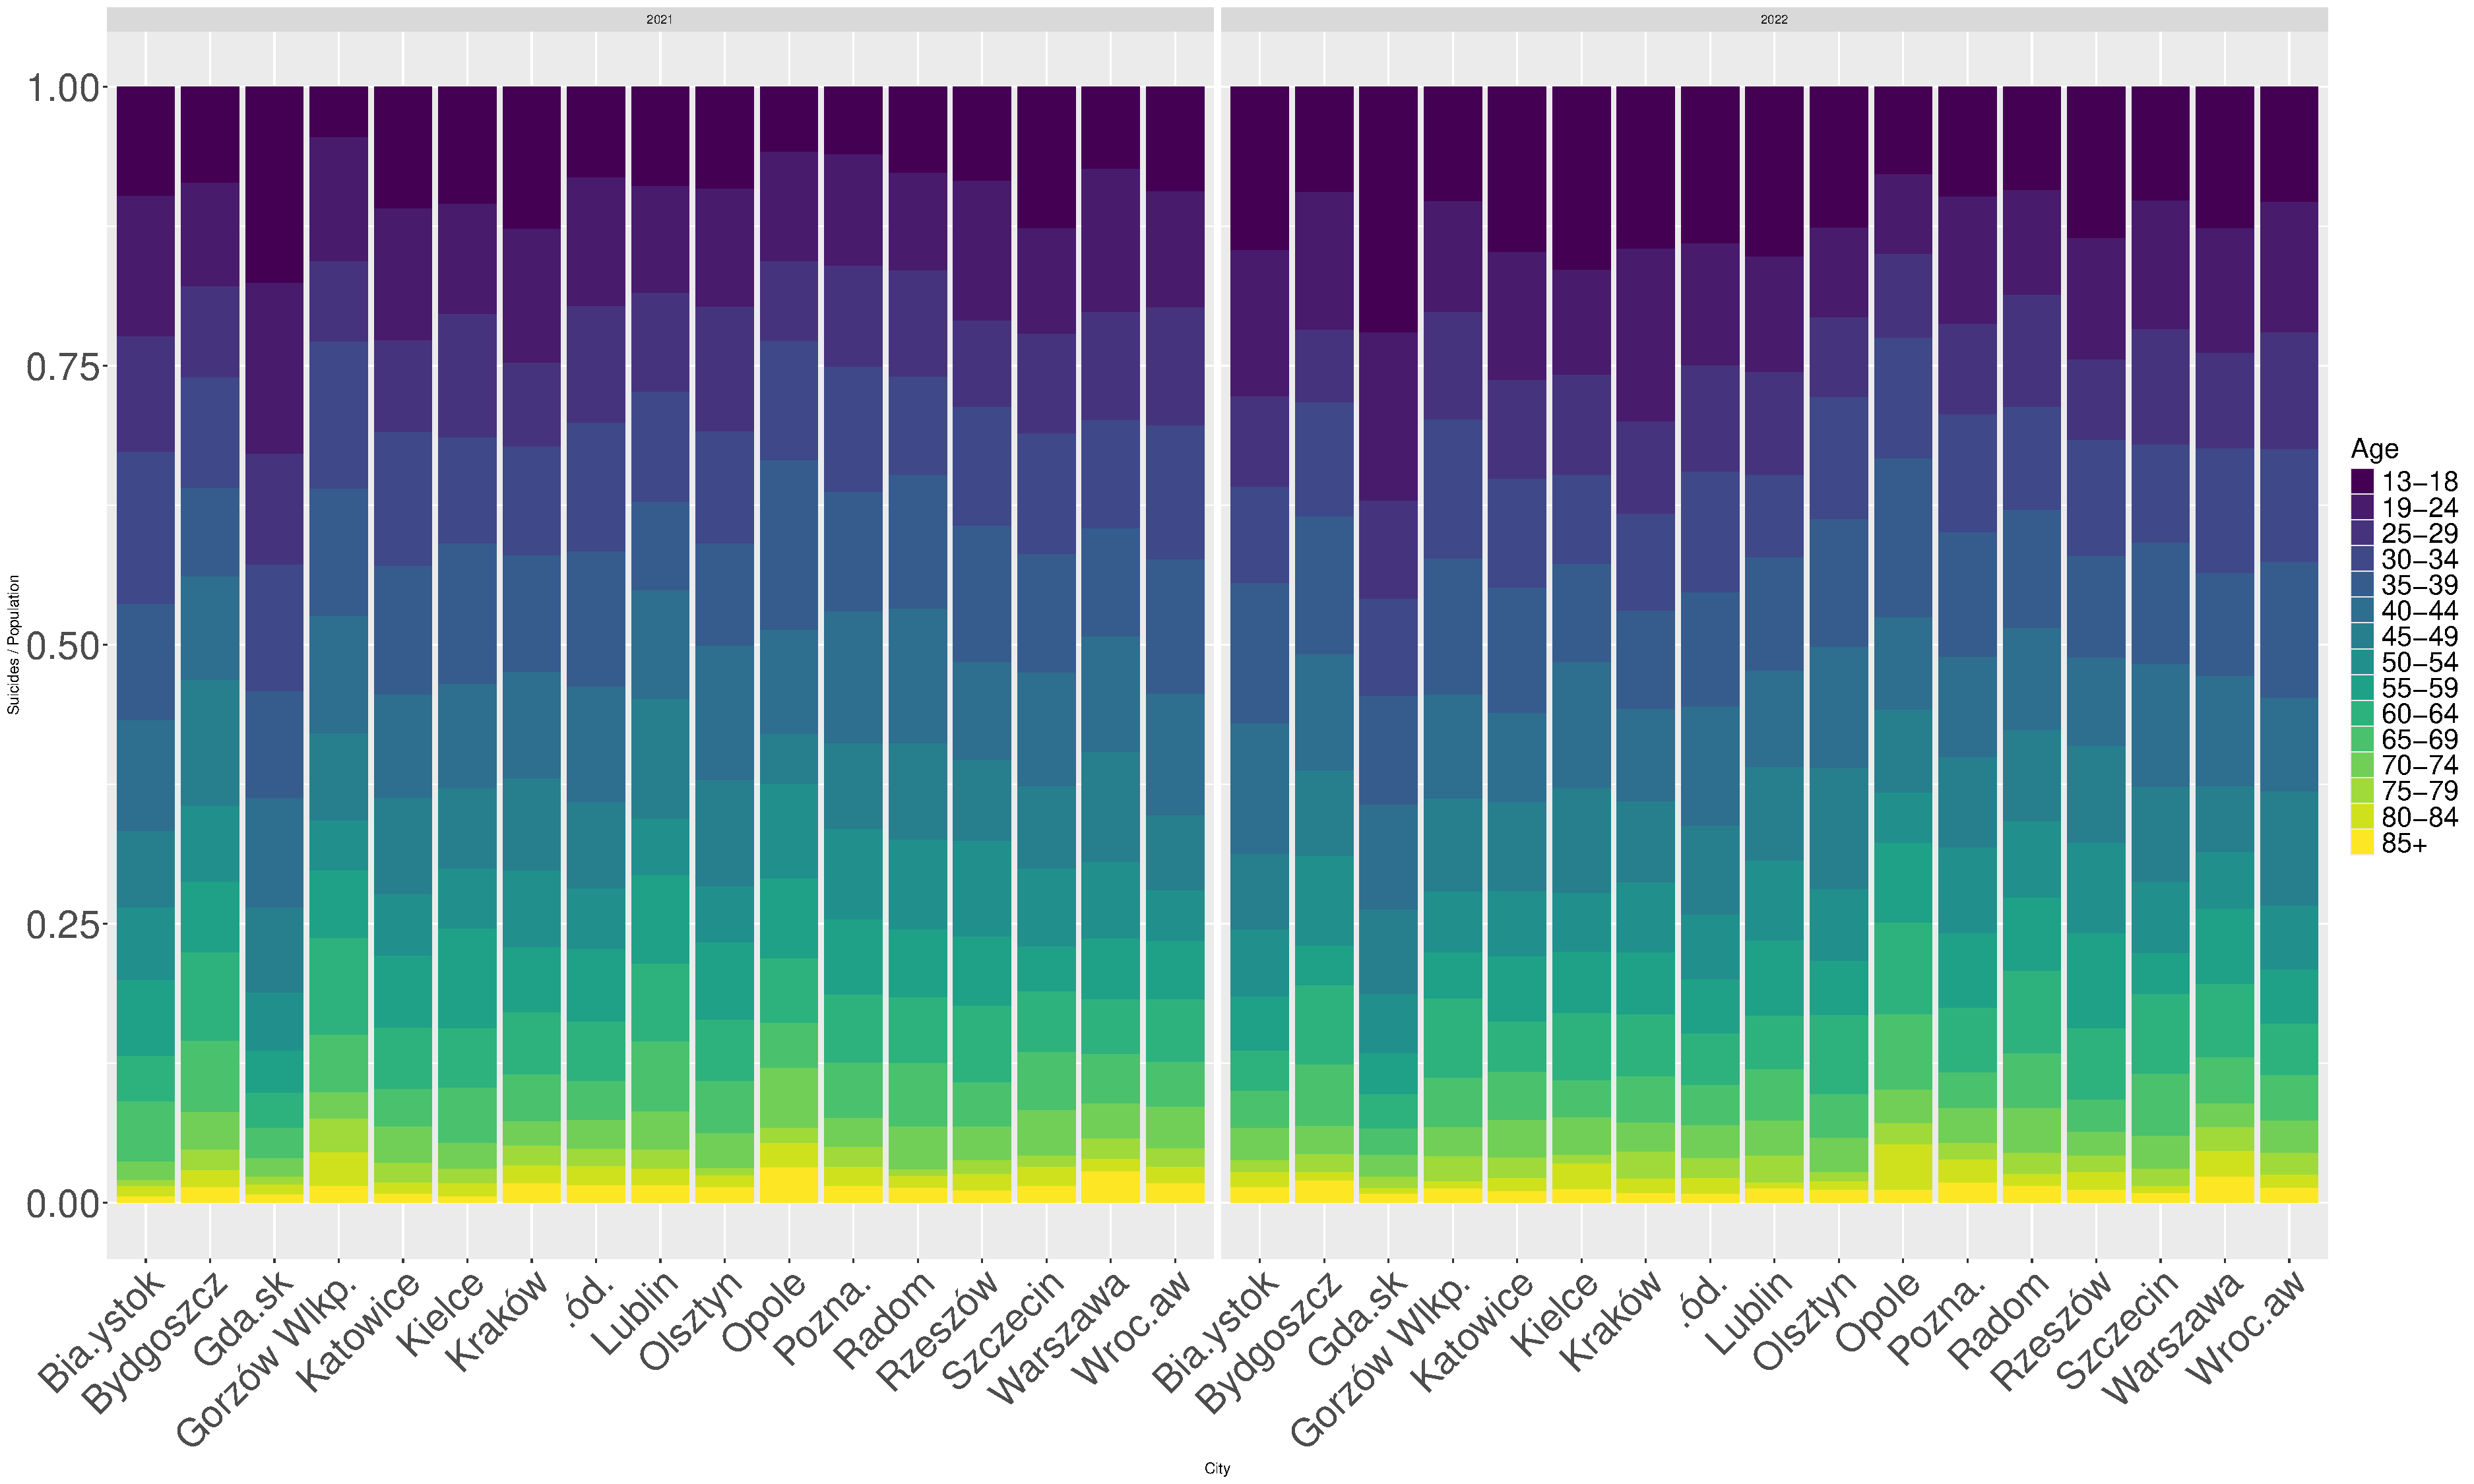
\includegraphics[width=0.65\textwidth]{imgs/age_city_op-2122.pdf}
    \caption{Attempted suicides by age range in 2021 and 2022}
    \label{fig:age_city_att_op-2122}
\end{figure}

\begin{figure}[H]
    \centering
    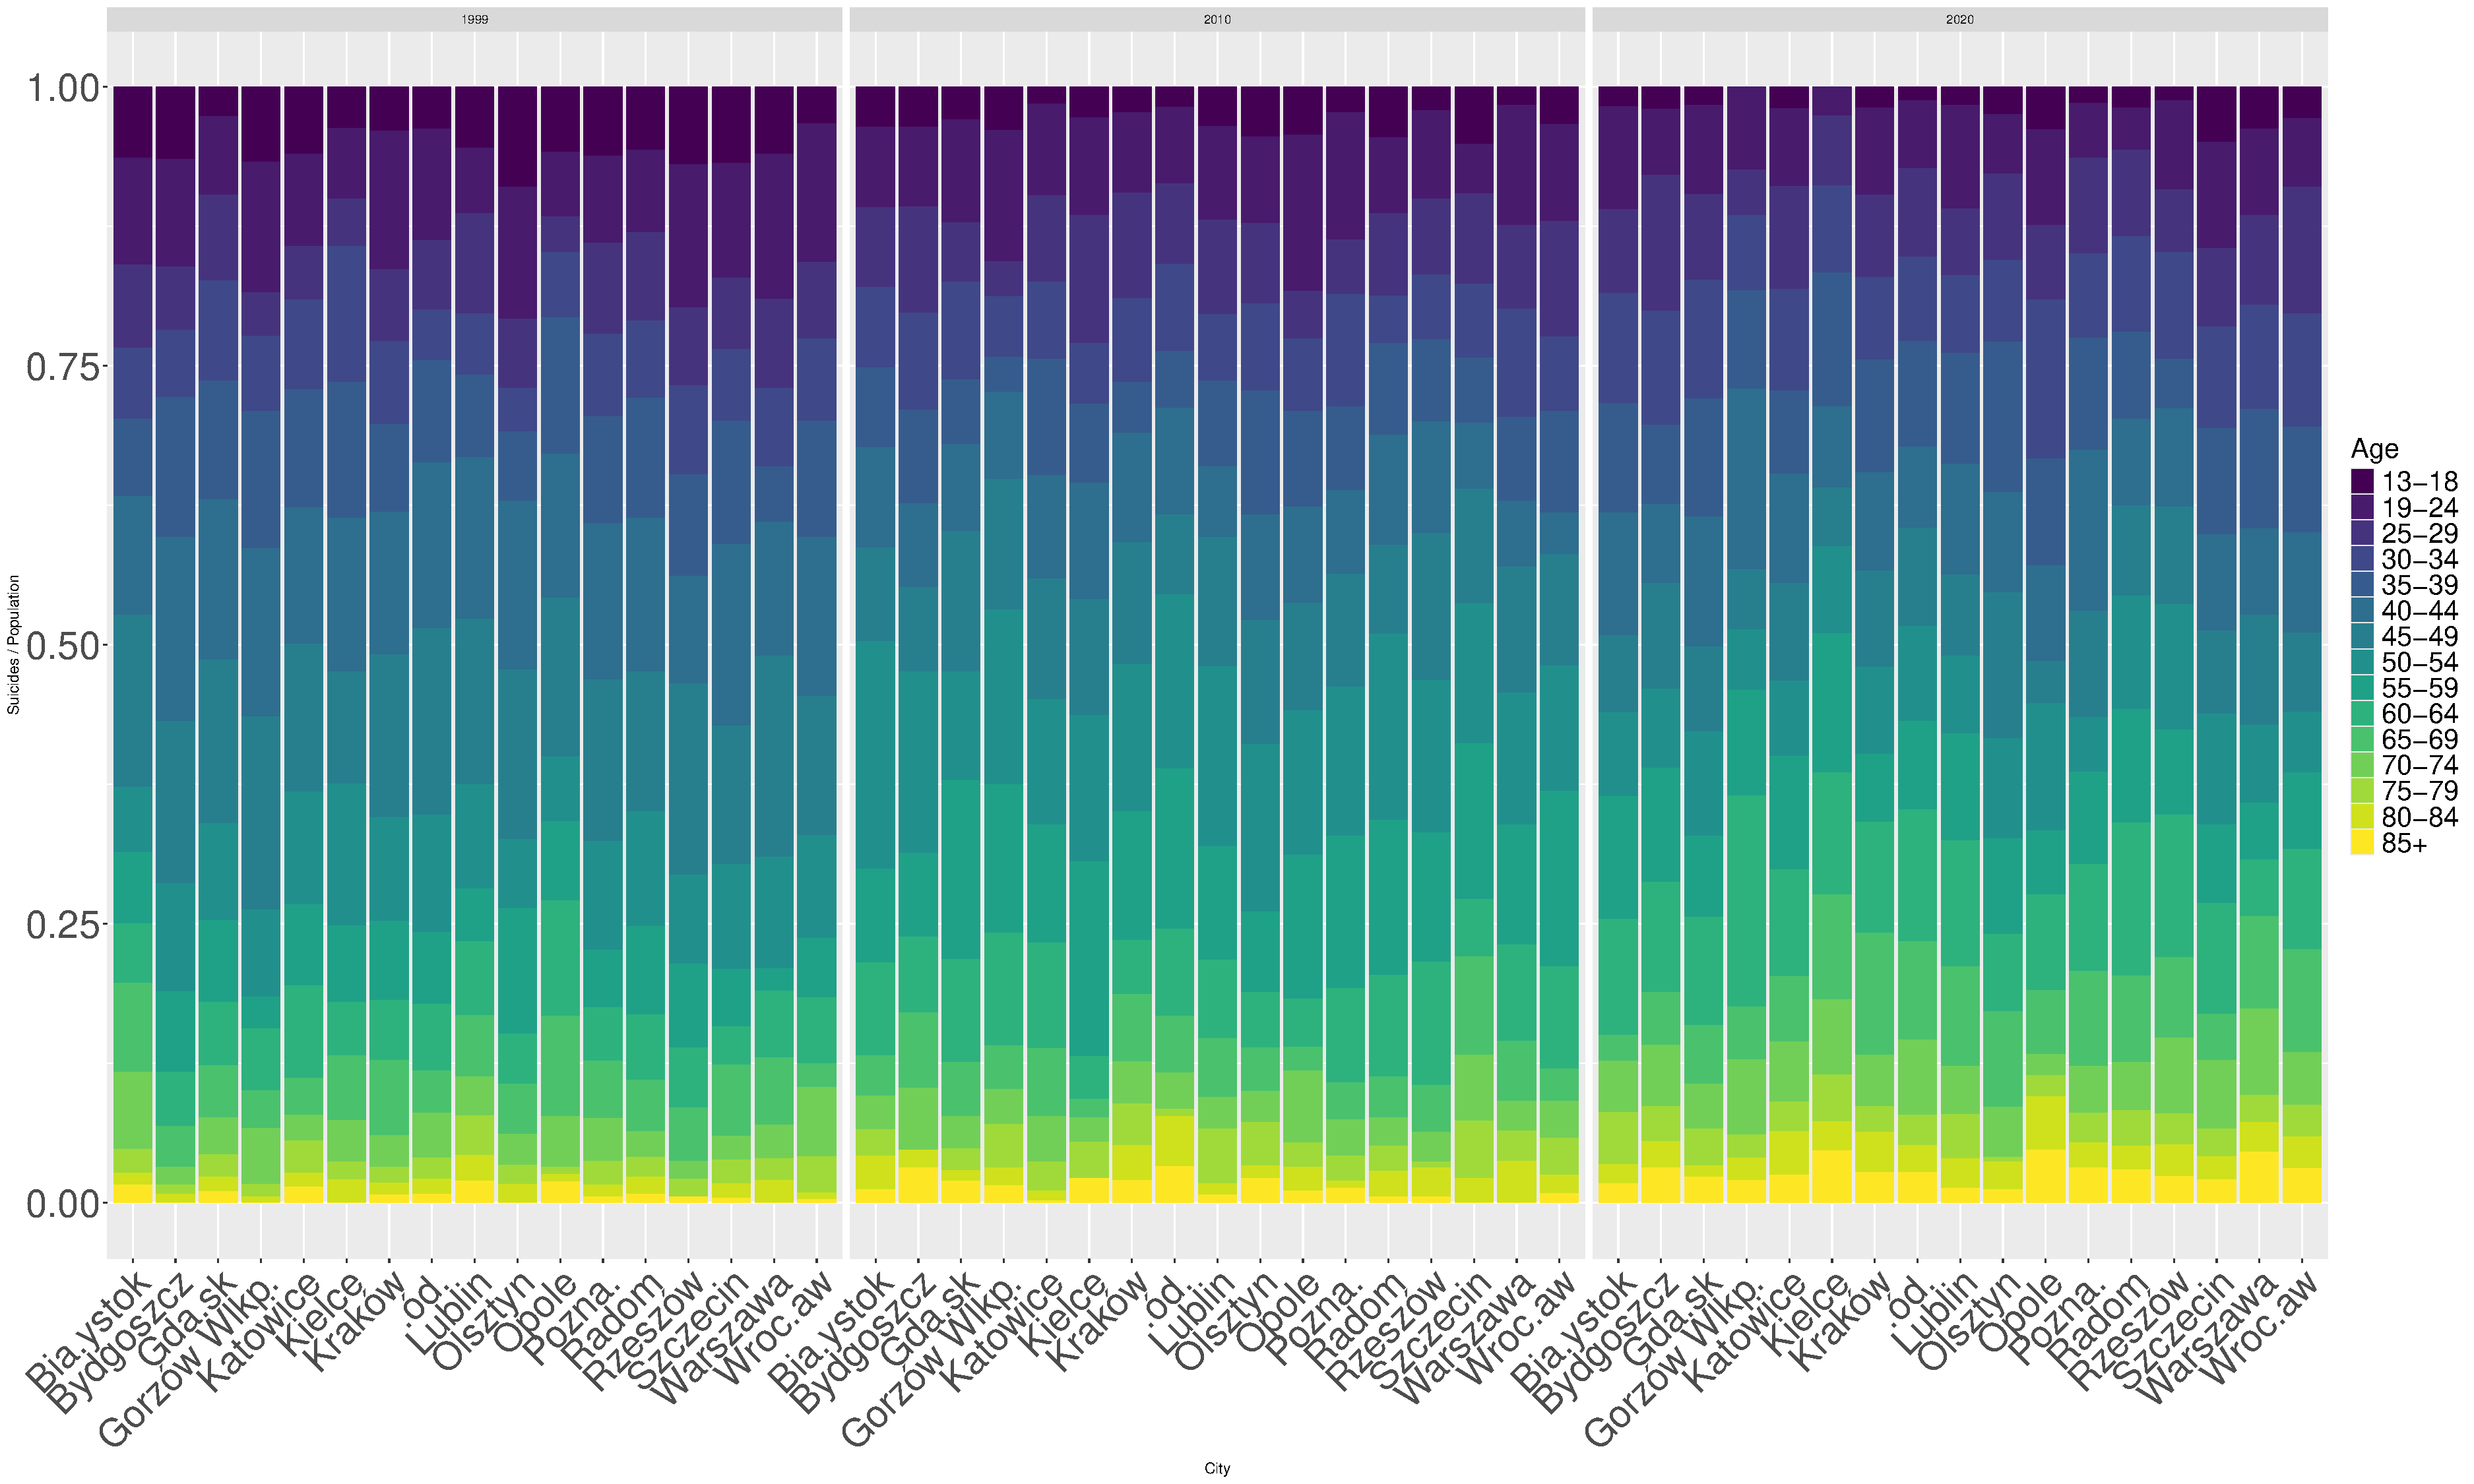
\includegraphics[width=0.65\textwidth]{imgs/age_city_fat_op-991020.pdf}
    \caption{Fatal suicides by age range in 1999, 2010 and 2020}
    \label{fig:age_city_fat_op-991020}
\end{figure}

\begin{figure}[H]
    \centering
    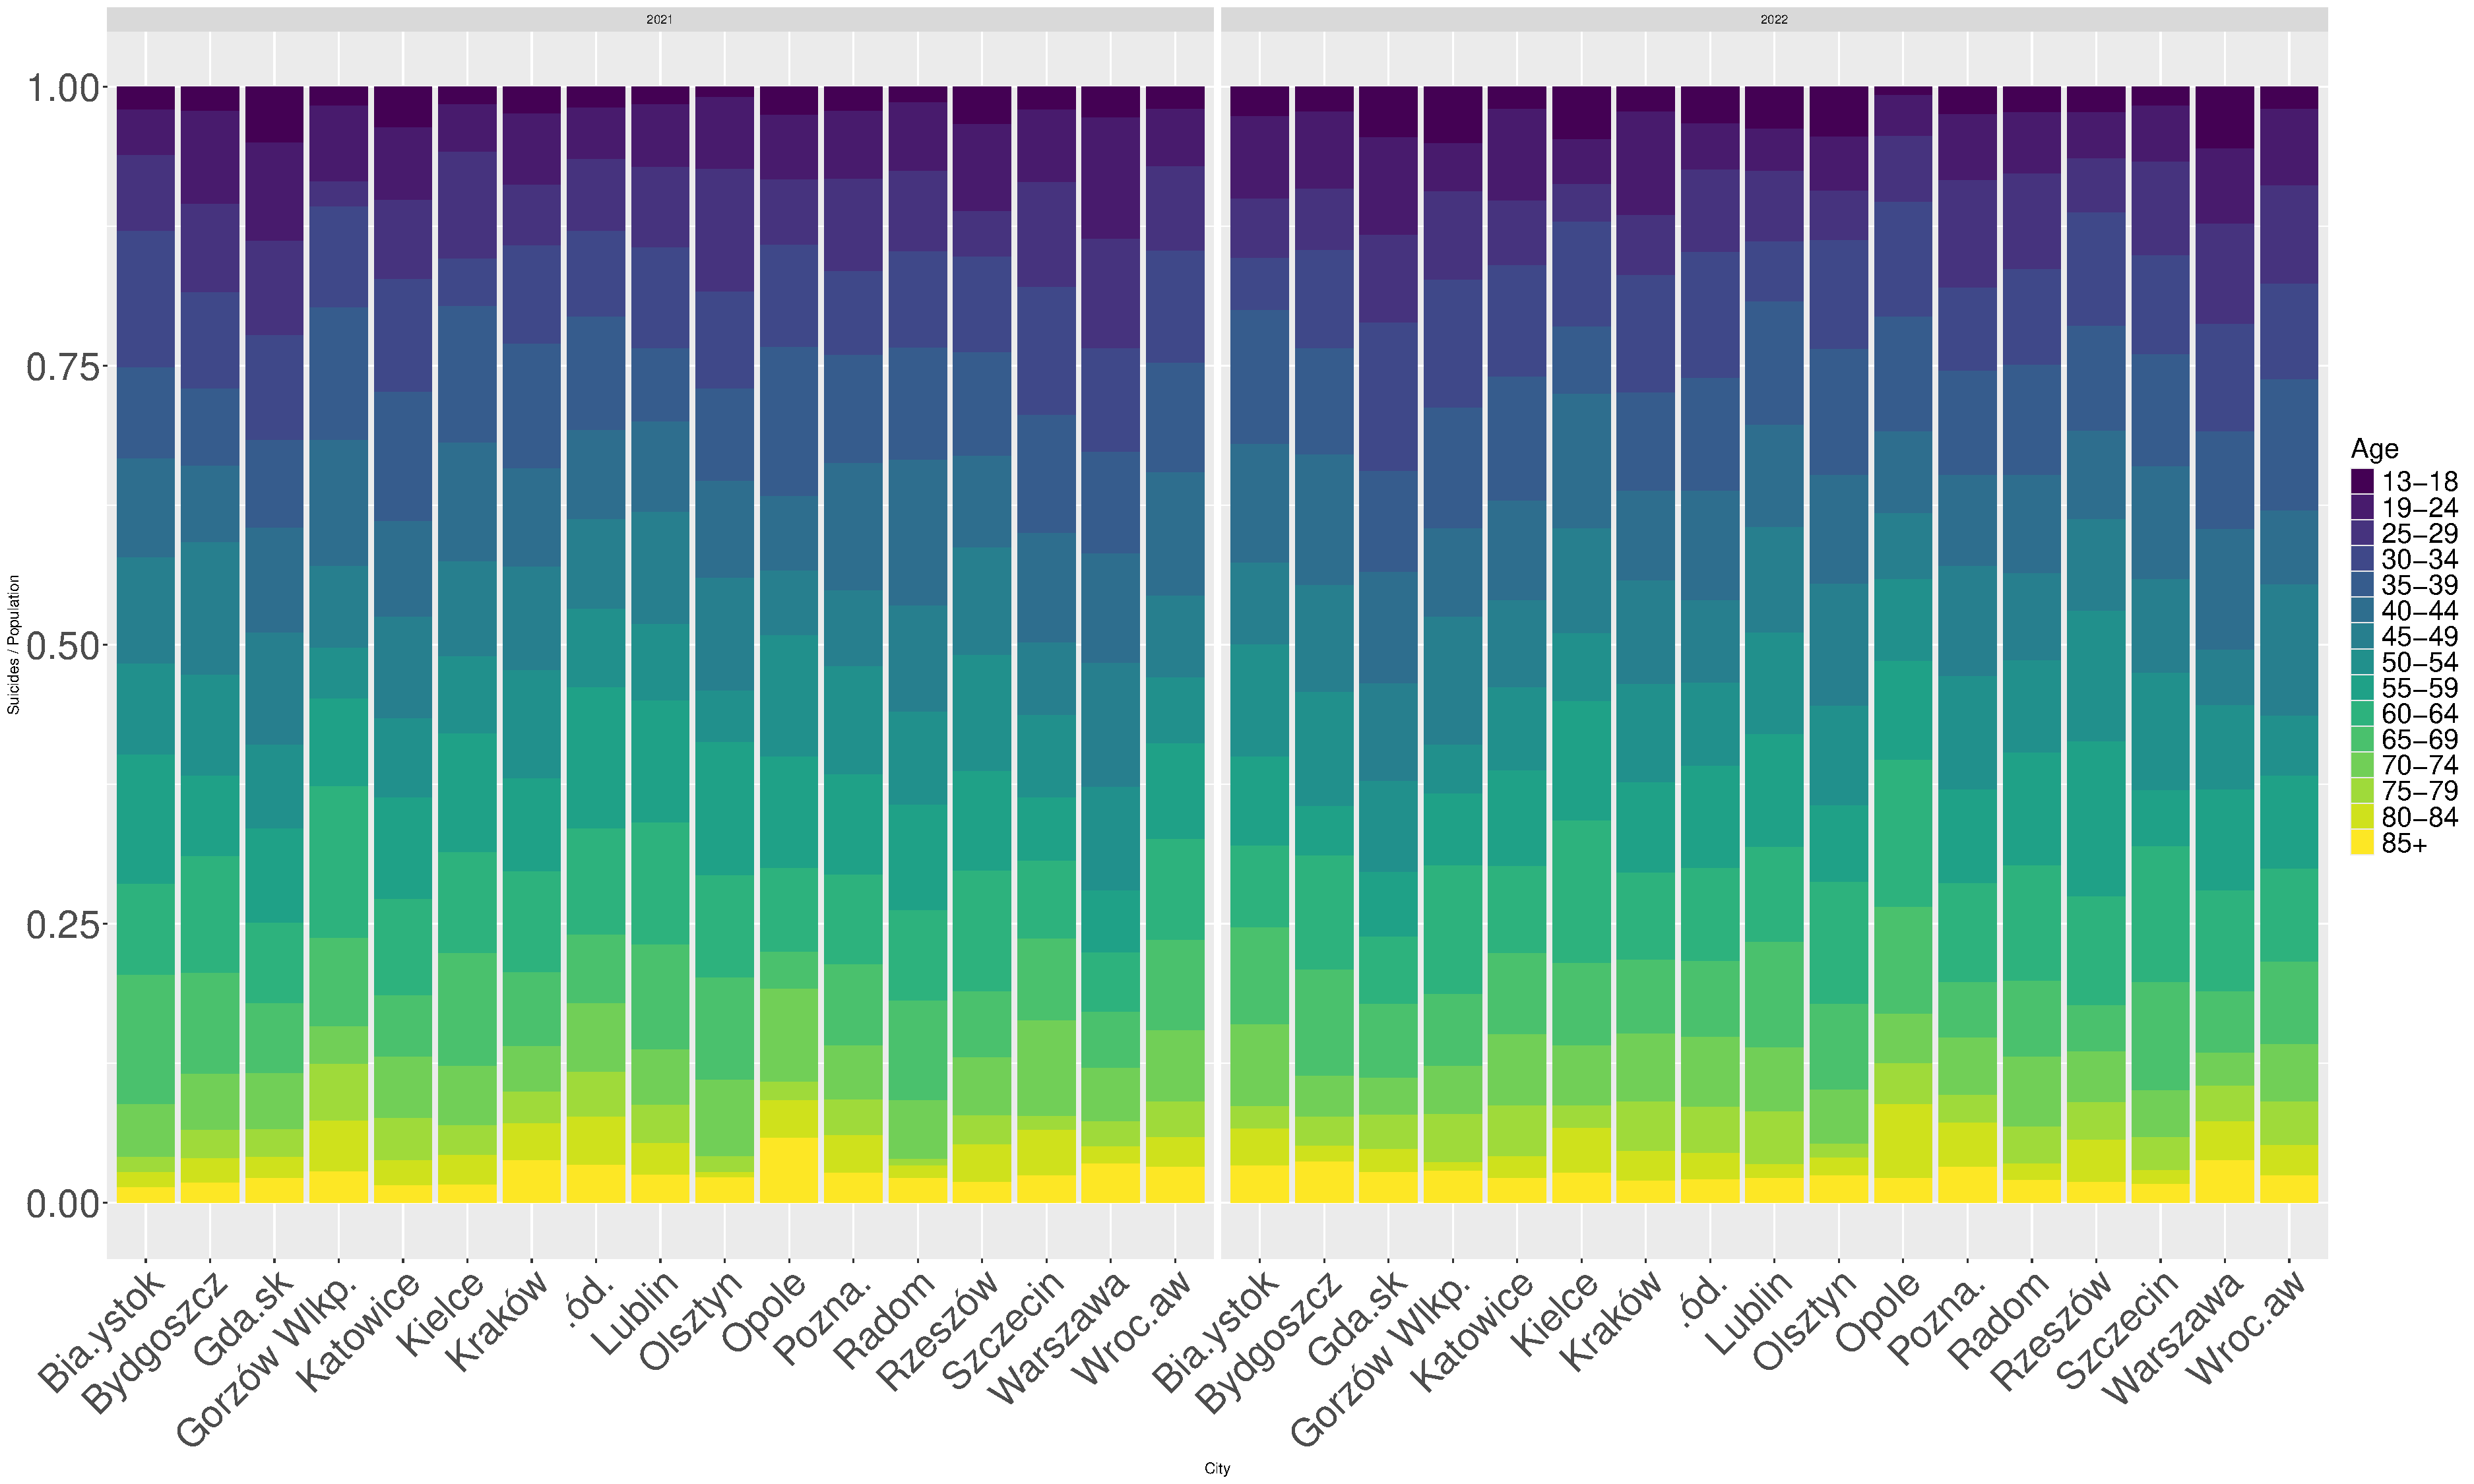
\includegraphics[width=0.65\textwidth]{imgs/age_city_fat_op-2122.pdf}
    \caption{Fatal suicides by age range in 2021 and 2022}
    \label{fig:age_city_fat_op-2122}
\end{figure}




Figures \ref{fig:age_city_op-att-2022}
and \ref{fig:age_city_op-fat-2022}
show that
the place where most people attempted suicide in 2022 is Katowice, 
in particular younger people, while focusing on fatal suicides 
also Radom and Rzeszów appear to be problematic places.
The least affected city appears to be Warszawa.
%
\begin{figure}[H]
    \centering
    \begin{minipage}{0.65\textwidth}
        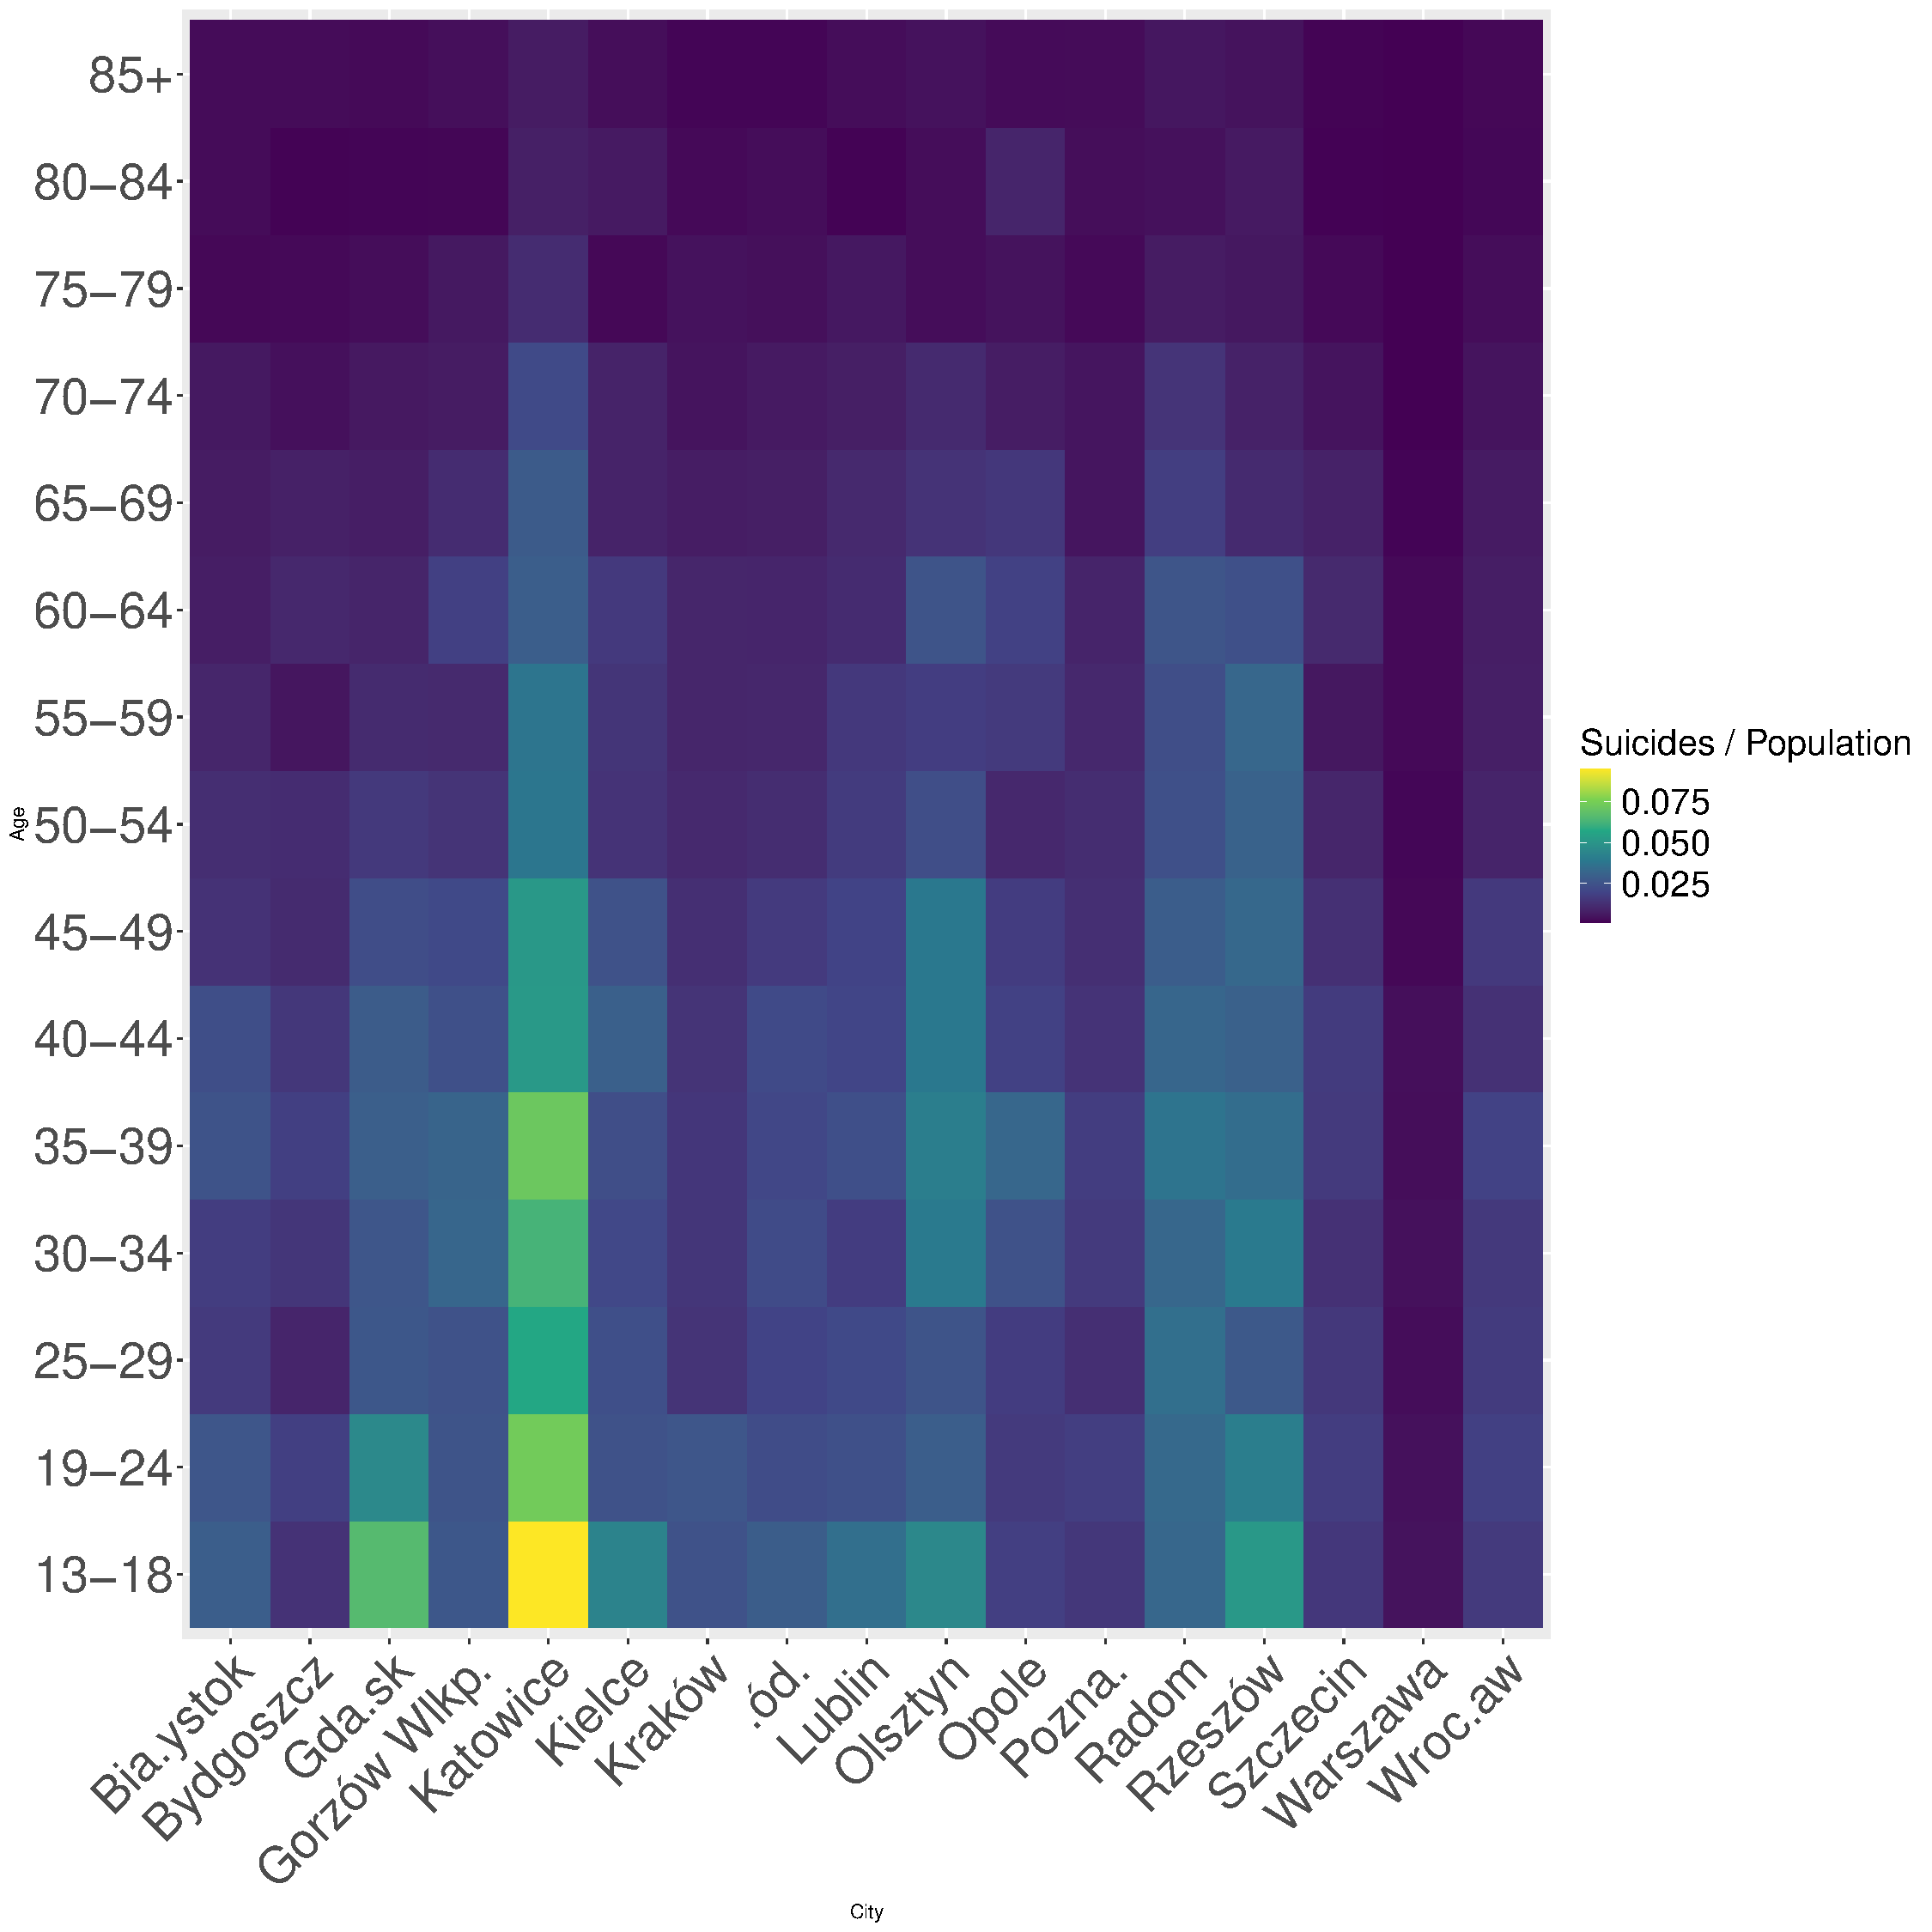
\includegraphics[width=\textwidth]{imgs/age_city_op-att-2022.pdf}
        \caption{Attempted suicides by age range in 2022 in different cities}
	\label{fig:age_city_op-att-2022}
    \end{minipage}
    \hfill
    \begin{minipage}{0.65\textwidth}
        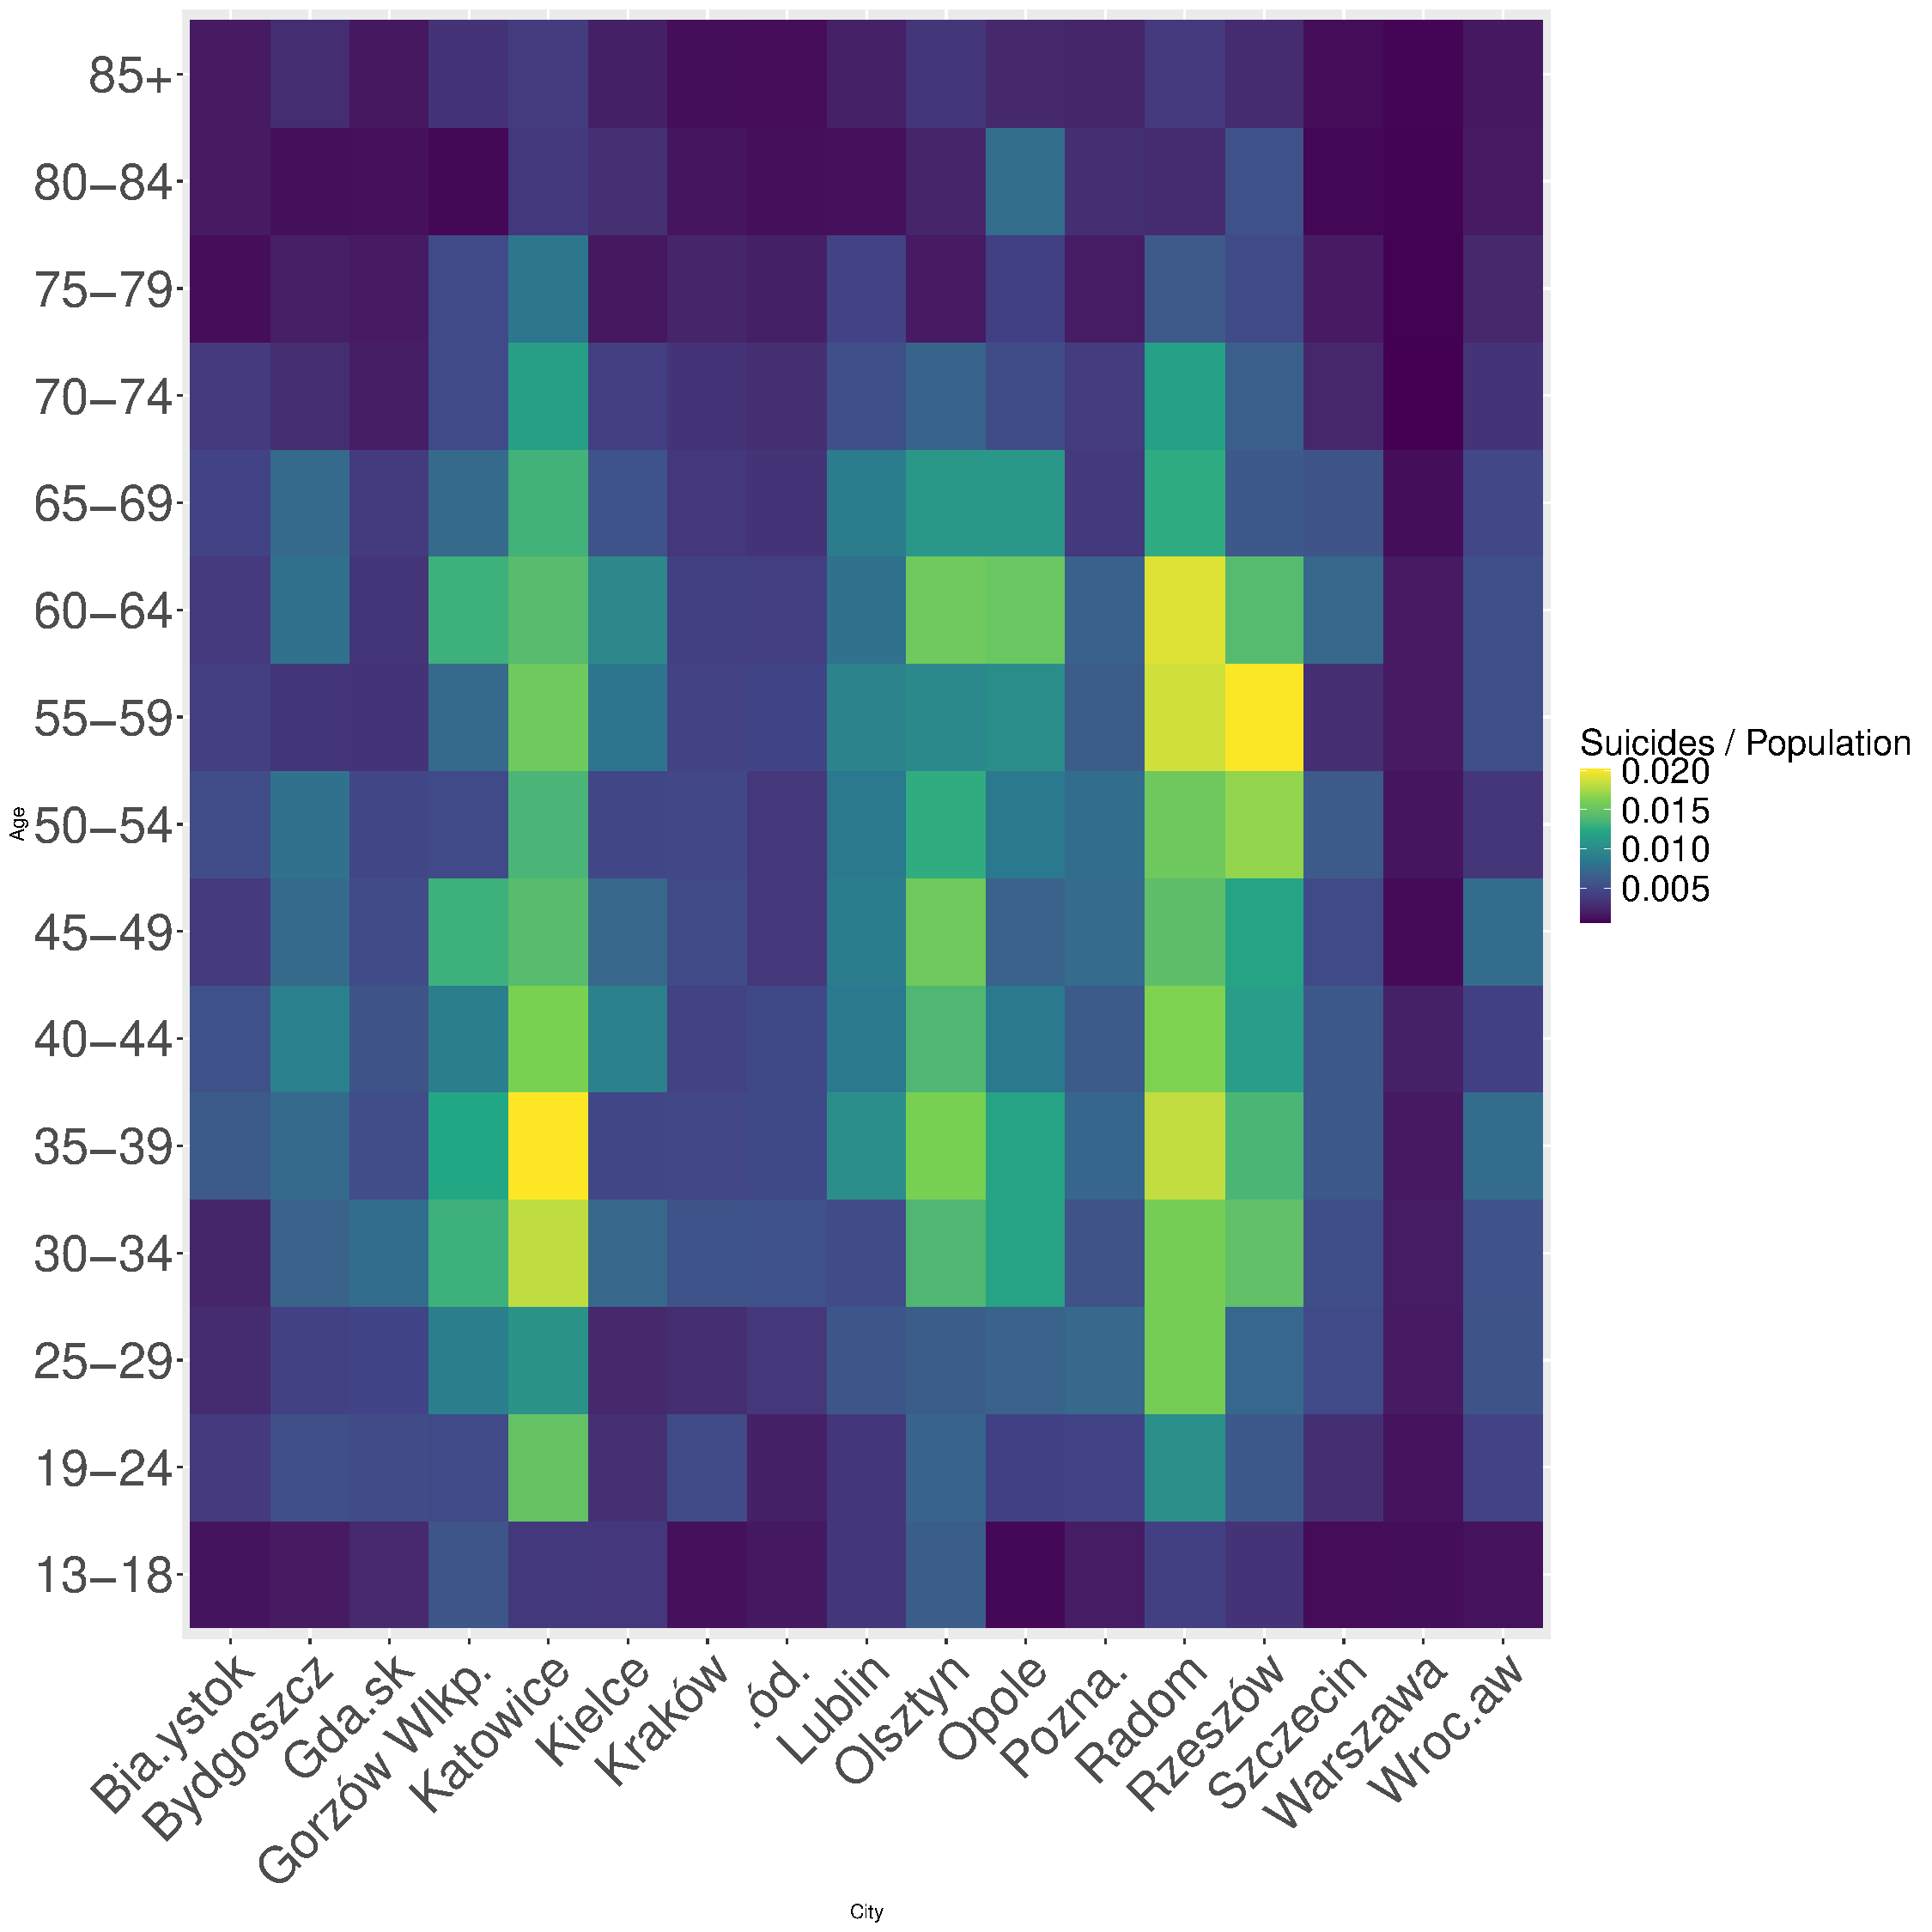
\includegraphics[width=\textwidth]{imgs/age_city_op-fat-2022.pdf}
        \caption{Fatal suicides by age range in 2022 in different cities}
	\label{fig:age_city_op-fat-2022}
    \end{minipage}
\end{figure}
%
%
%

%
\subsection{Sex}
Figures \ref{fig:sex_attempted}, \ref{fig:sex_fatal}, \ref{fig:sex_foa}
show that the two trends of attempted and fatal suicides for males and females
are quite similar up until 2013, with less abrupt changes for females but still
increasing and decreasing in the same years men did, then a worrying trend of attempted 
suicides of women starts after 2017 and it unfortunately reflects in an increment
in the number of fatal suicides of women starting from 2018 whereas men, starting from 2019, show a decrease.
It is important to remark that the condition of women in Poland still needs improvements,
unfortunately some political choices made during the last years did not help \footnotemark{}:
\begin{quote}
\textit{The court removed the right to abortions because of birth defects, 
which had accounted for more than 90\% of all abortions. Since January 2021, 
abortion has been allowed only in cases of rape, incest or when a mother's 
health is in danger.}
\end{quote}
\footnotetext{\url{https://theconversation.com/why-polands-new-government-is-challenged-by-abortion-228863}}
%
\begin{figure}[H]
    \centering
    \begin{minipage}{0.65\textwidth}
        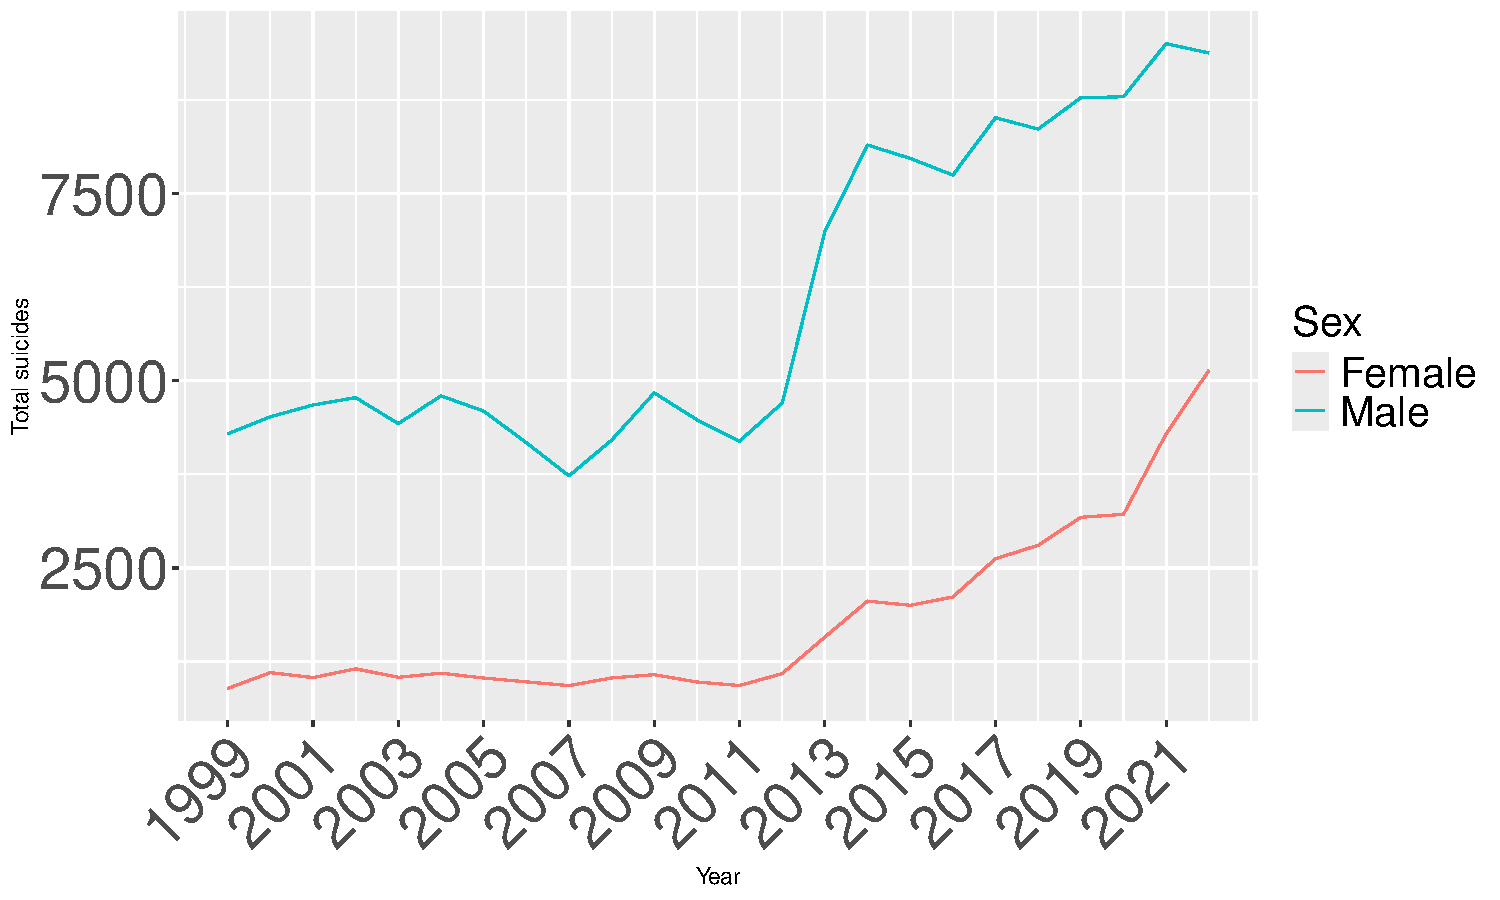
\includegraphics[width=\textwidth]{imgs/sex_attempted.pdf}
        \caption{Trend of attempted suicides by sex }
	\label{fig:sex_attempted}
    \end{minipage}
    \hfill
    \begin{minipage}{0.65\textwidth}
        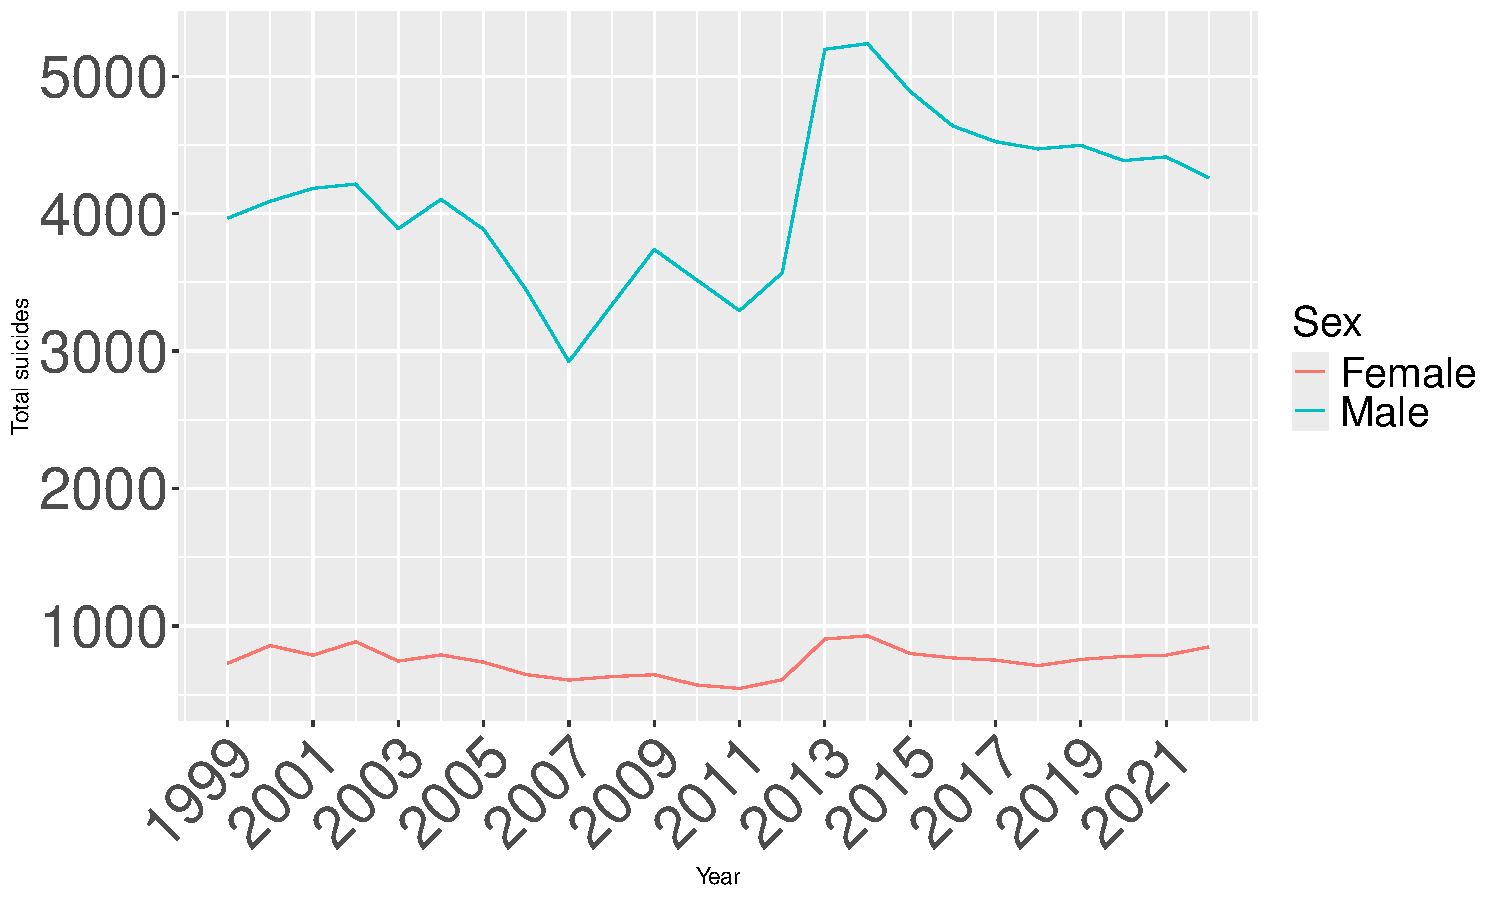
\includegraphics[width=\textwidth]{imgs/sex_fatal.pdf}
        \caption{Trend of fatal suicides by sex }
	\label{fig:sex_fatal}
    \end{minipage}
\end{figure}

\begin{figure}[H]
    \centering
    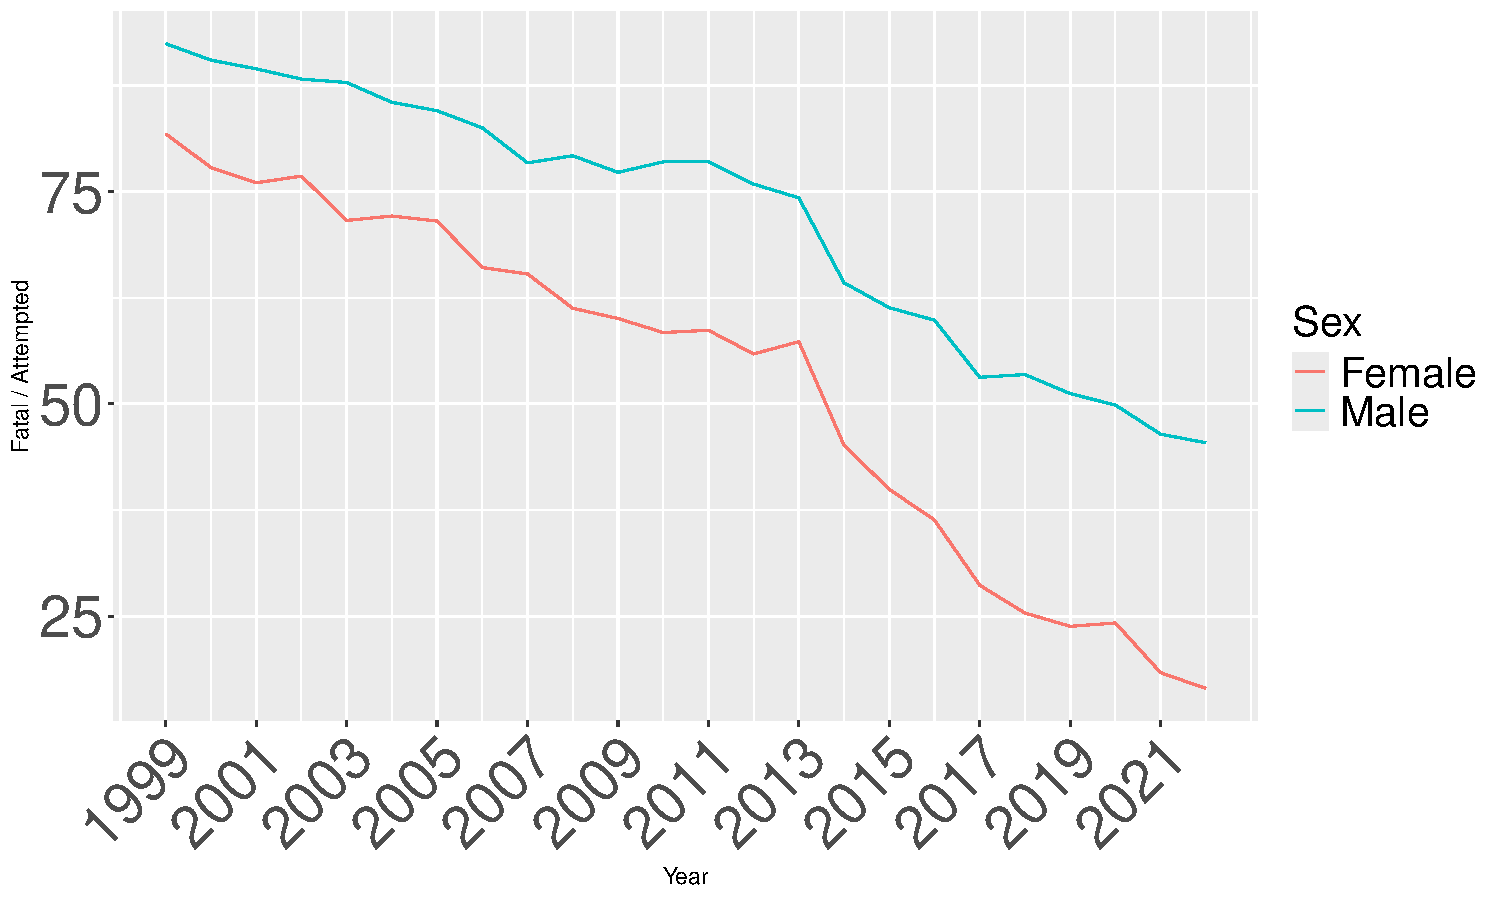
\includegraphics[width=0.65\textwidth]{imgs/sex_foa.pdf}
    \caption{Trend of fatal over attempted suicides by sex }
    \label{fig:sex_foa}
\end{figure}

\begin{figure}[H]
    \centering
    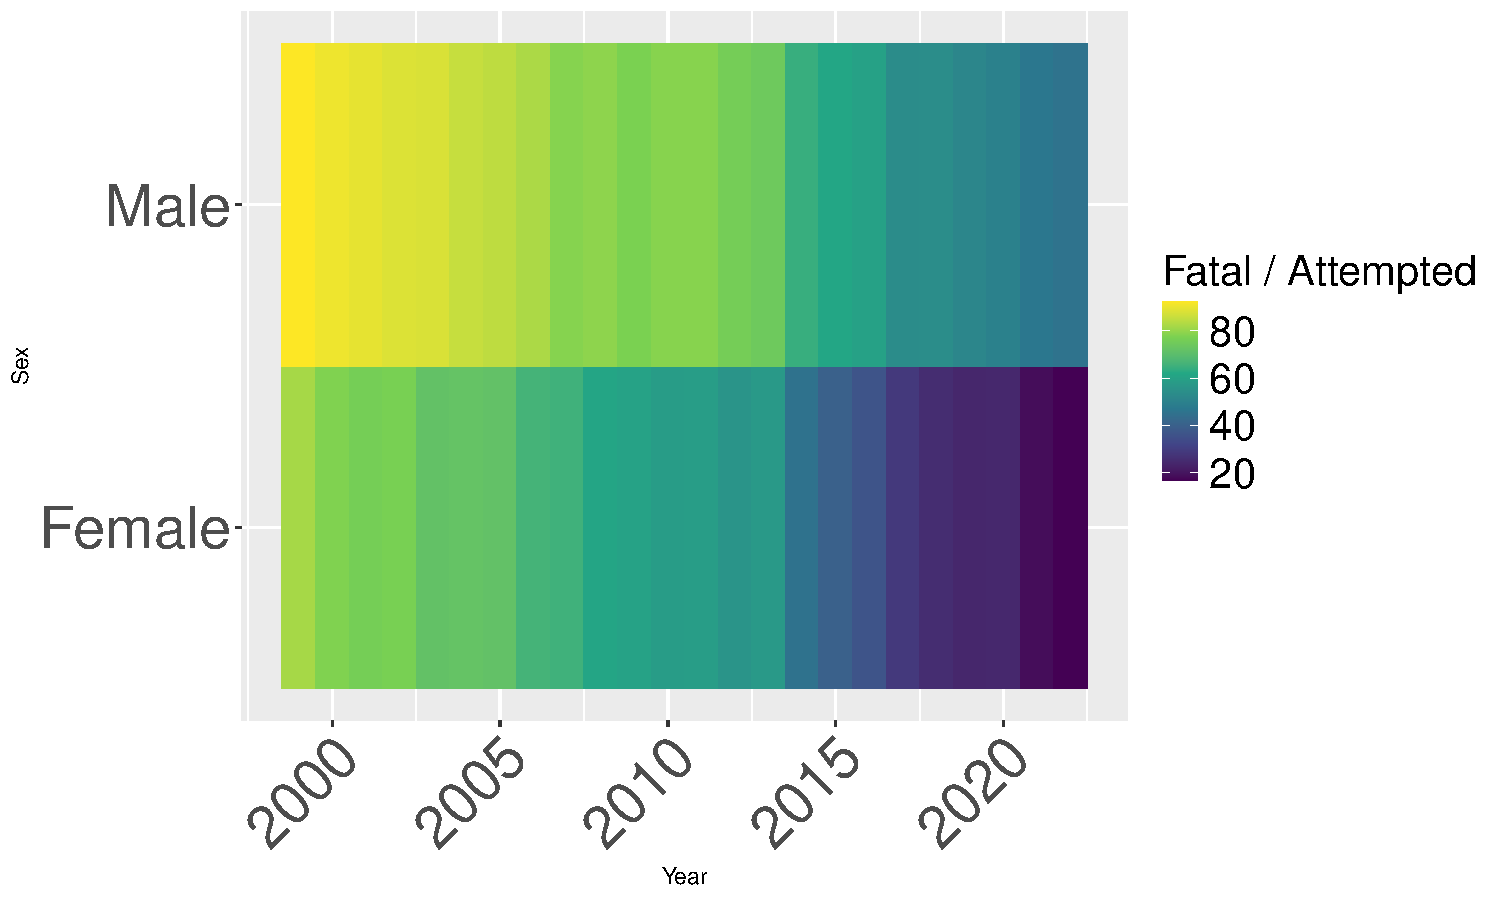
\includegraphics[width=0.65\textwidth]{imgs/sex_foa_heat.pdf}
    \caption{Heatmap of fatal over attempted suicides by sex}
    \label{fig:sex_foa_heat}
\end{figure}
%
%
Figure \ref{fig:sex_foa_heat} shows that in general women are less likely to commit
suicide when attempting.
%
From figure \ref{fig:sex_city_att_suicides-991020} it is not easy to spot a city in particular
where disparity between women and men is more present than in others,
Białystok, Szczecin and Warszawa are among the cities with a higher percentage
of women attempting suicide, the peak in Łódż in 2020 does not seem to be part of a trend.
Figure \ref{fig:sex_city_att_suicides-2122} shows that women's condition in Łódż worsened,
but the most problematic city became Gdańsk.
Figures \ref{fig:sex_city_fat_suicides-991020} and \ref{fig:sex_city_fat_suicides-2122}
seem to contradict the sad situation for women in Gdańsk and suggest that Warszawa
in 2022 had the worst condition for women to live, but in actuality what the barplots tell is
that in Warszawa it is more likely that women end up dead when attempting suicide,
this does not suggest by any means that Gdańsk has less serious social issues that lead
to depression.
Figure \ref{fig:sex_foa_city-2122} shows that the places where women are more likely to die 
when attempting 
suicide are Bydgoszcz and Warszawa but, similarly to what suggested above, 
this is independent from sex since those two cities are also the places where males are
more likely to end up dead when attempting suicide.
It is worth to investigate why in Gdańsk there were so many suicide attempts by women.
%
%
%
\begin{figure}[H]
    \centering
    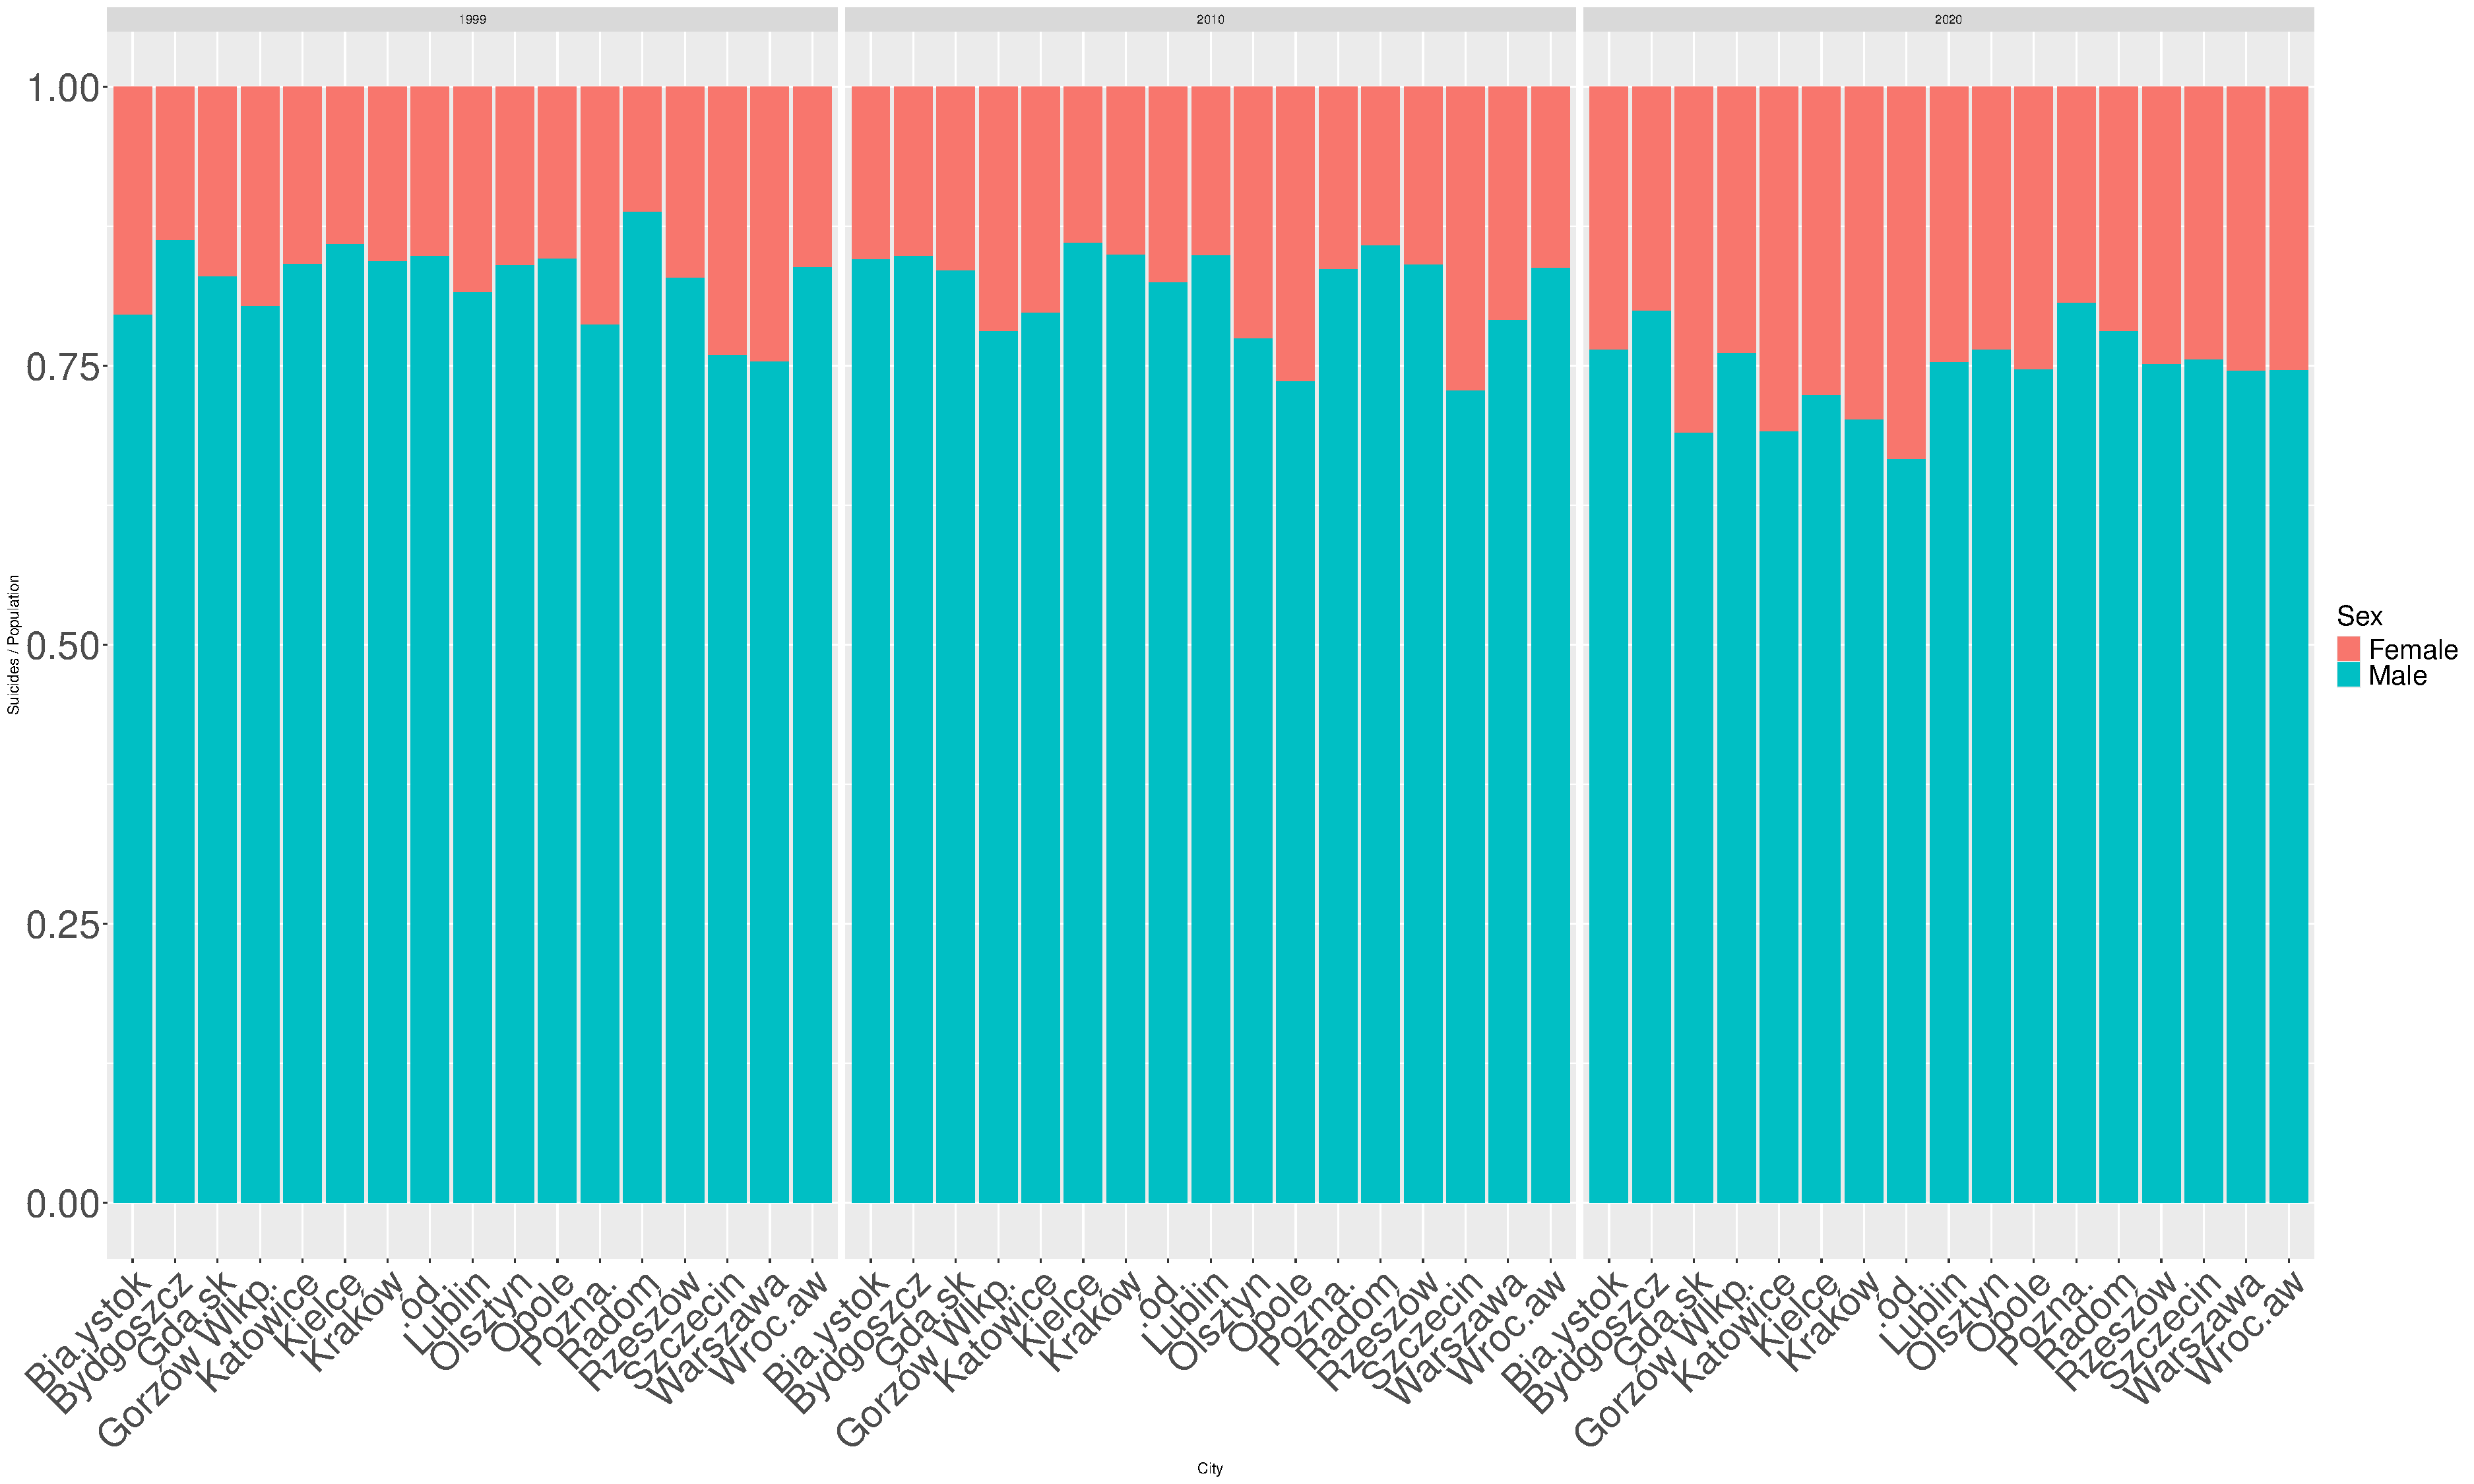
\includegraphics[width=0.65\textwidth]{imgs/sex_city_att_suicides-991020.pdf}
    \caption{Attempted suicides by sex  in 1999, 2010 and 2020}
    \label{fig:sex_city_att_suicides-991020}
\end{figure}

\begin{figure}[H]
    \centering
    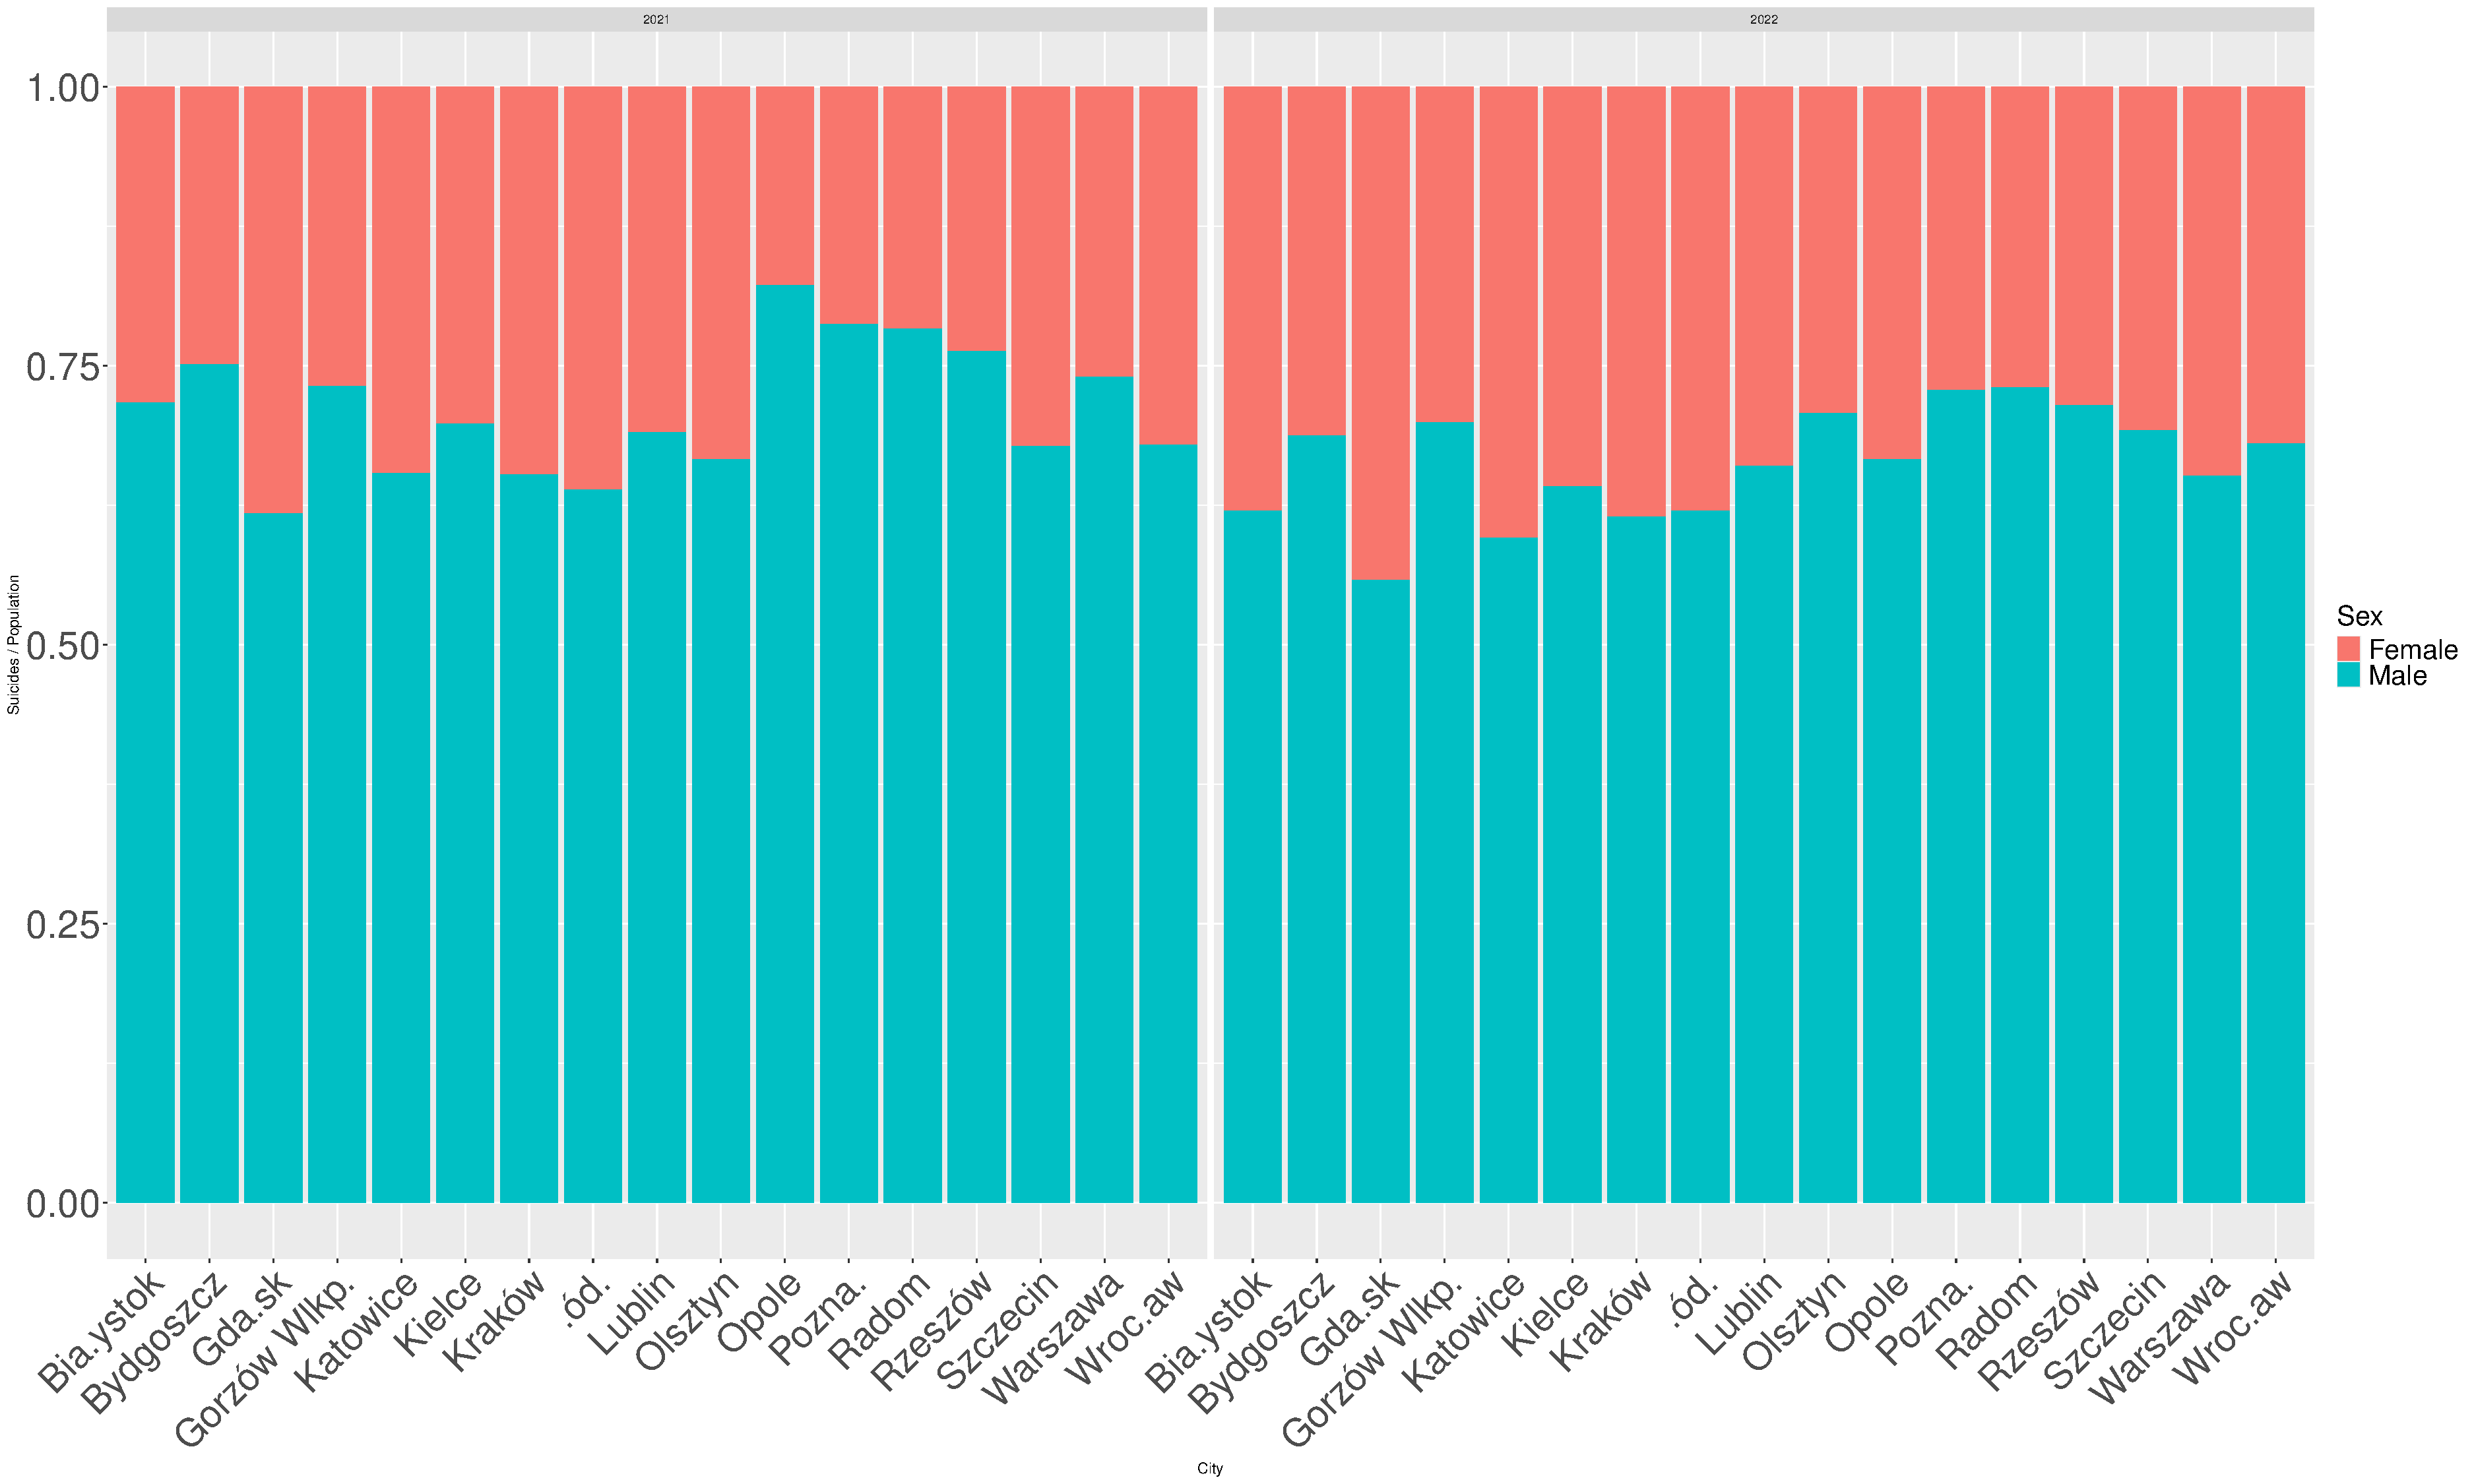
\includegraphics[width=0.65\textwidth]{imgs/sex_city_att_suicides-2122.pdf}
    \caption{Attempted suicides by sex  in 2021 and 2022}
    \label{fig:sex_city_att_suicides-2122}
\end{figure}

\begin{figure}[H]
    \centering
    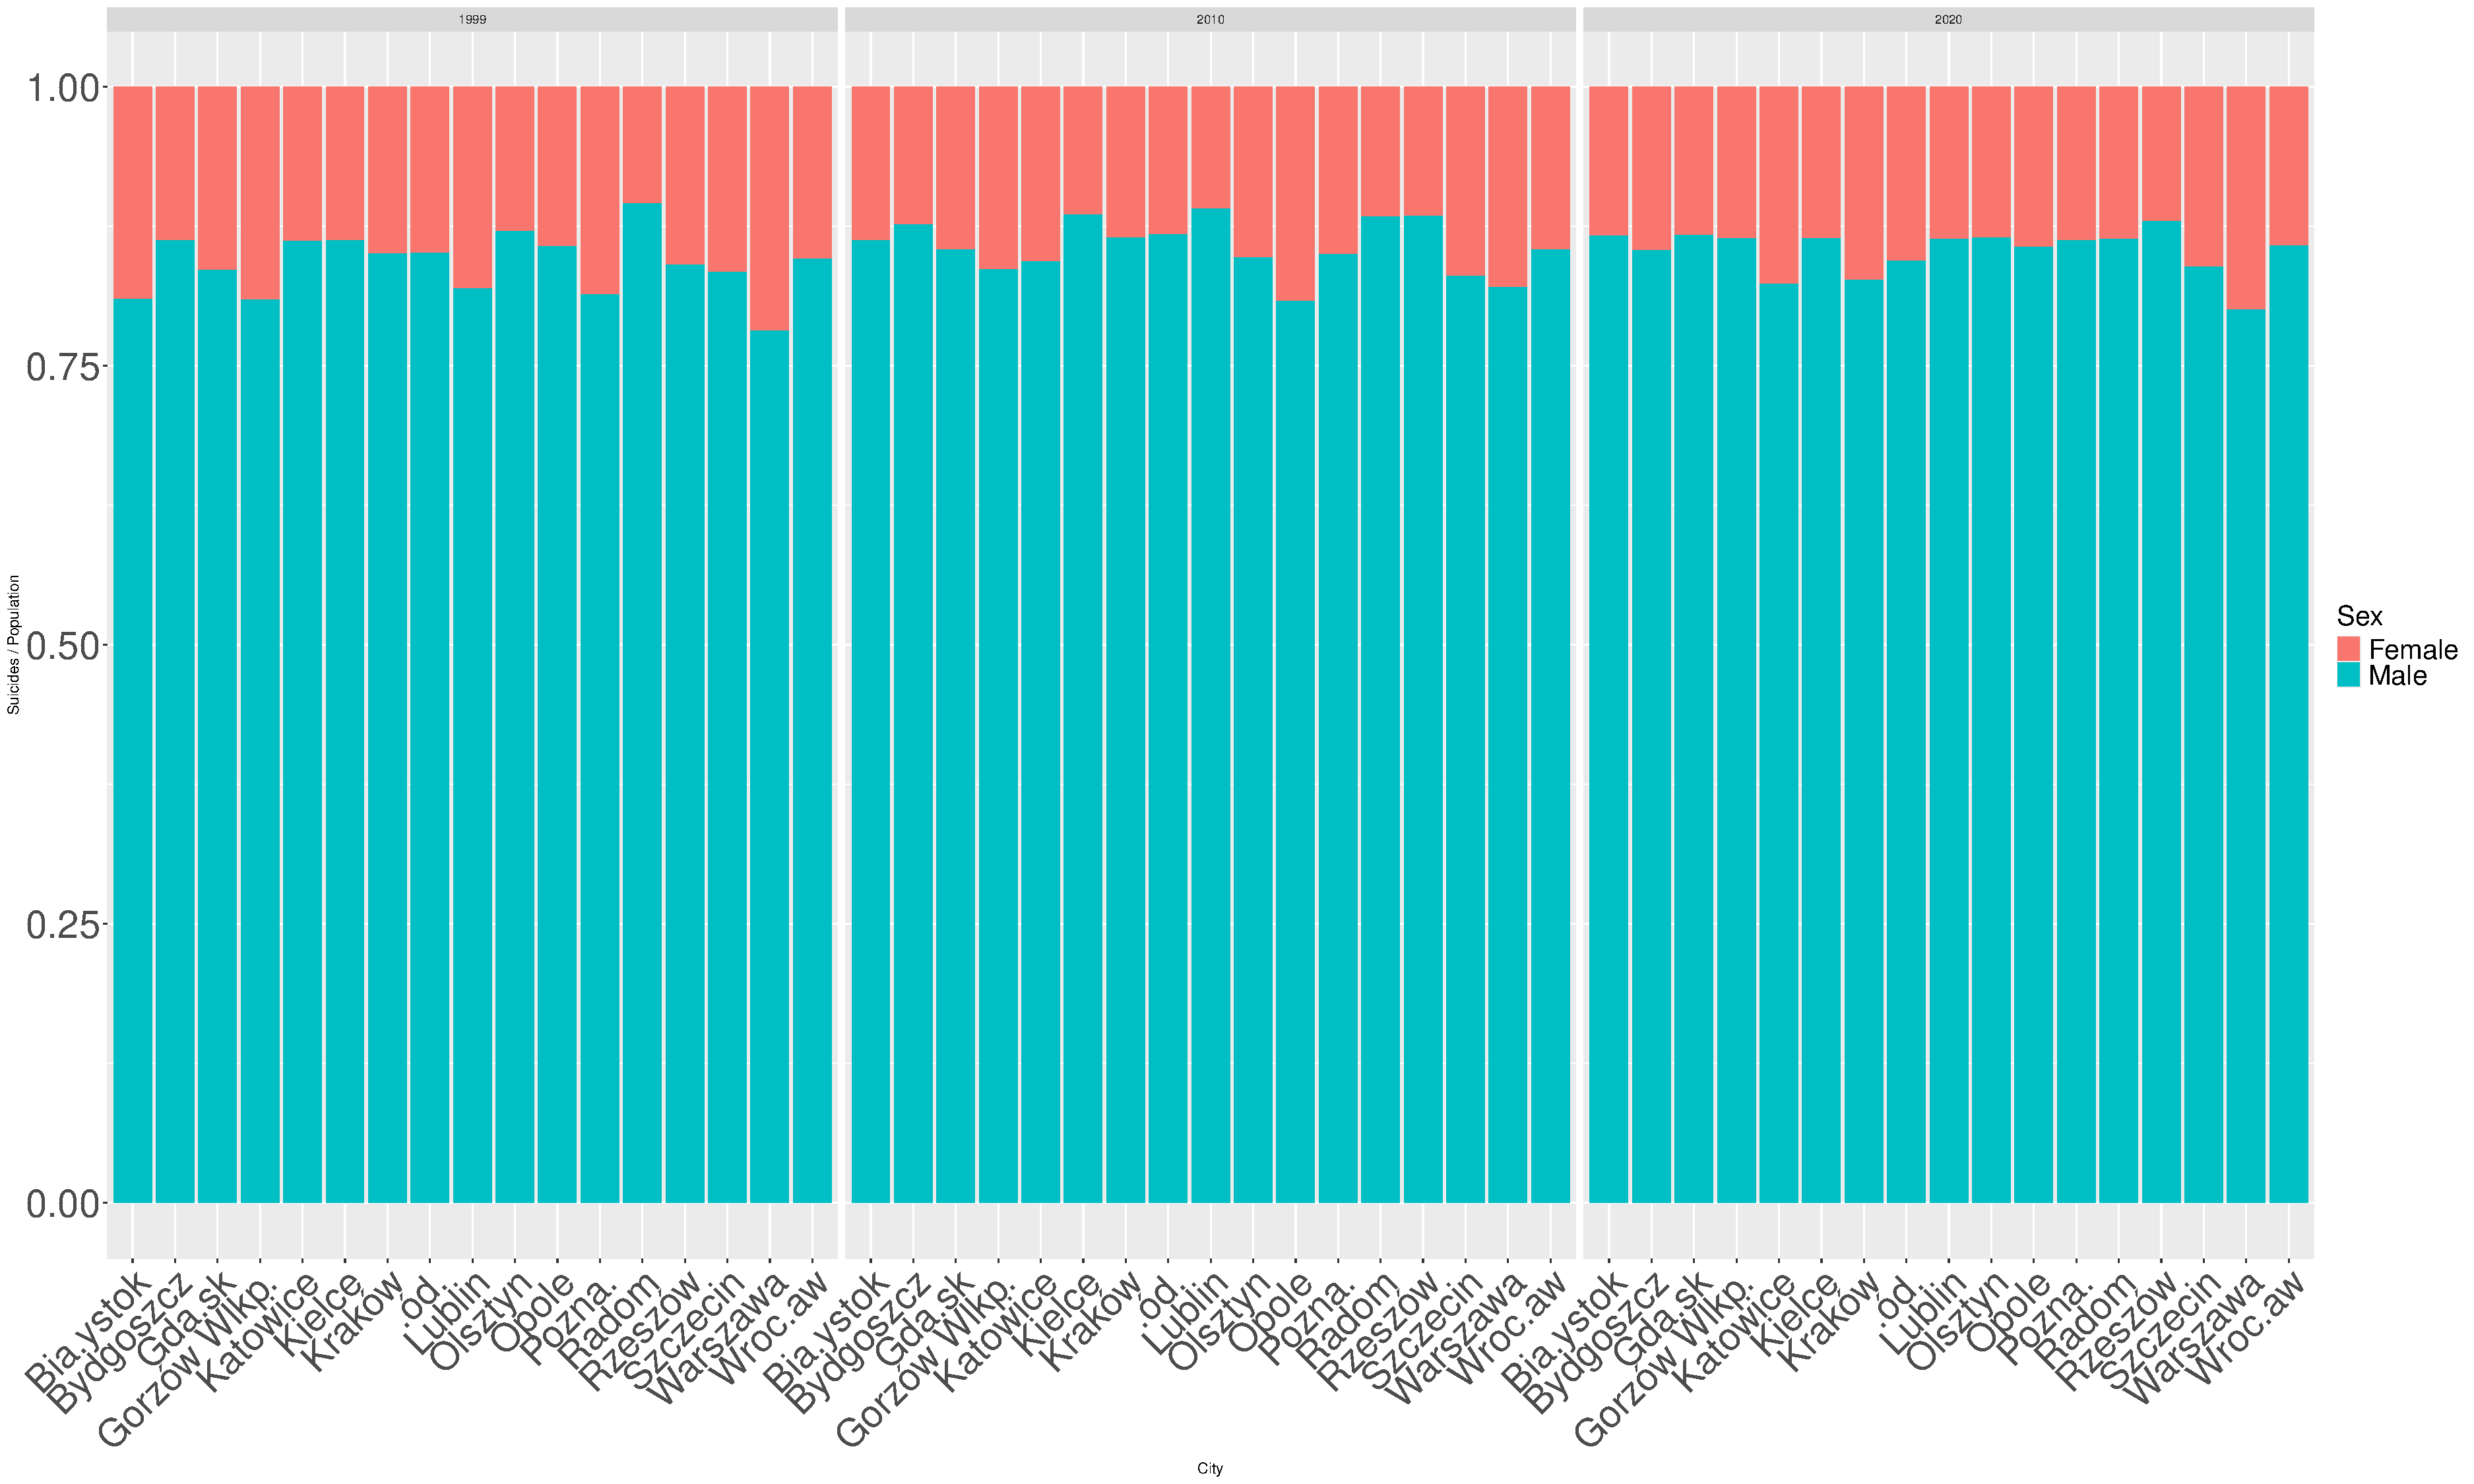
\includegraphics[width=0.65\textwidth]{imgs/sex_city_fat_suicides-991020.pdf}
    \caption{Fatal suicides by sex  in 1999, 2010 and 2020}
    \label{fig:sex_city_fat_suicides-991020}
\end{figure}

\begin{figure}[H]
    \centering
    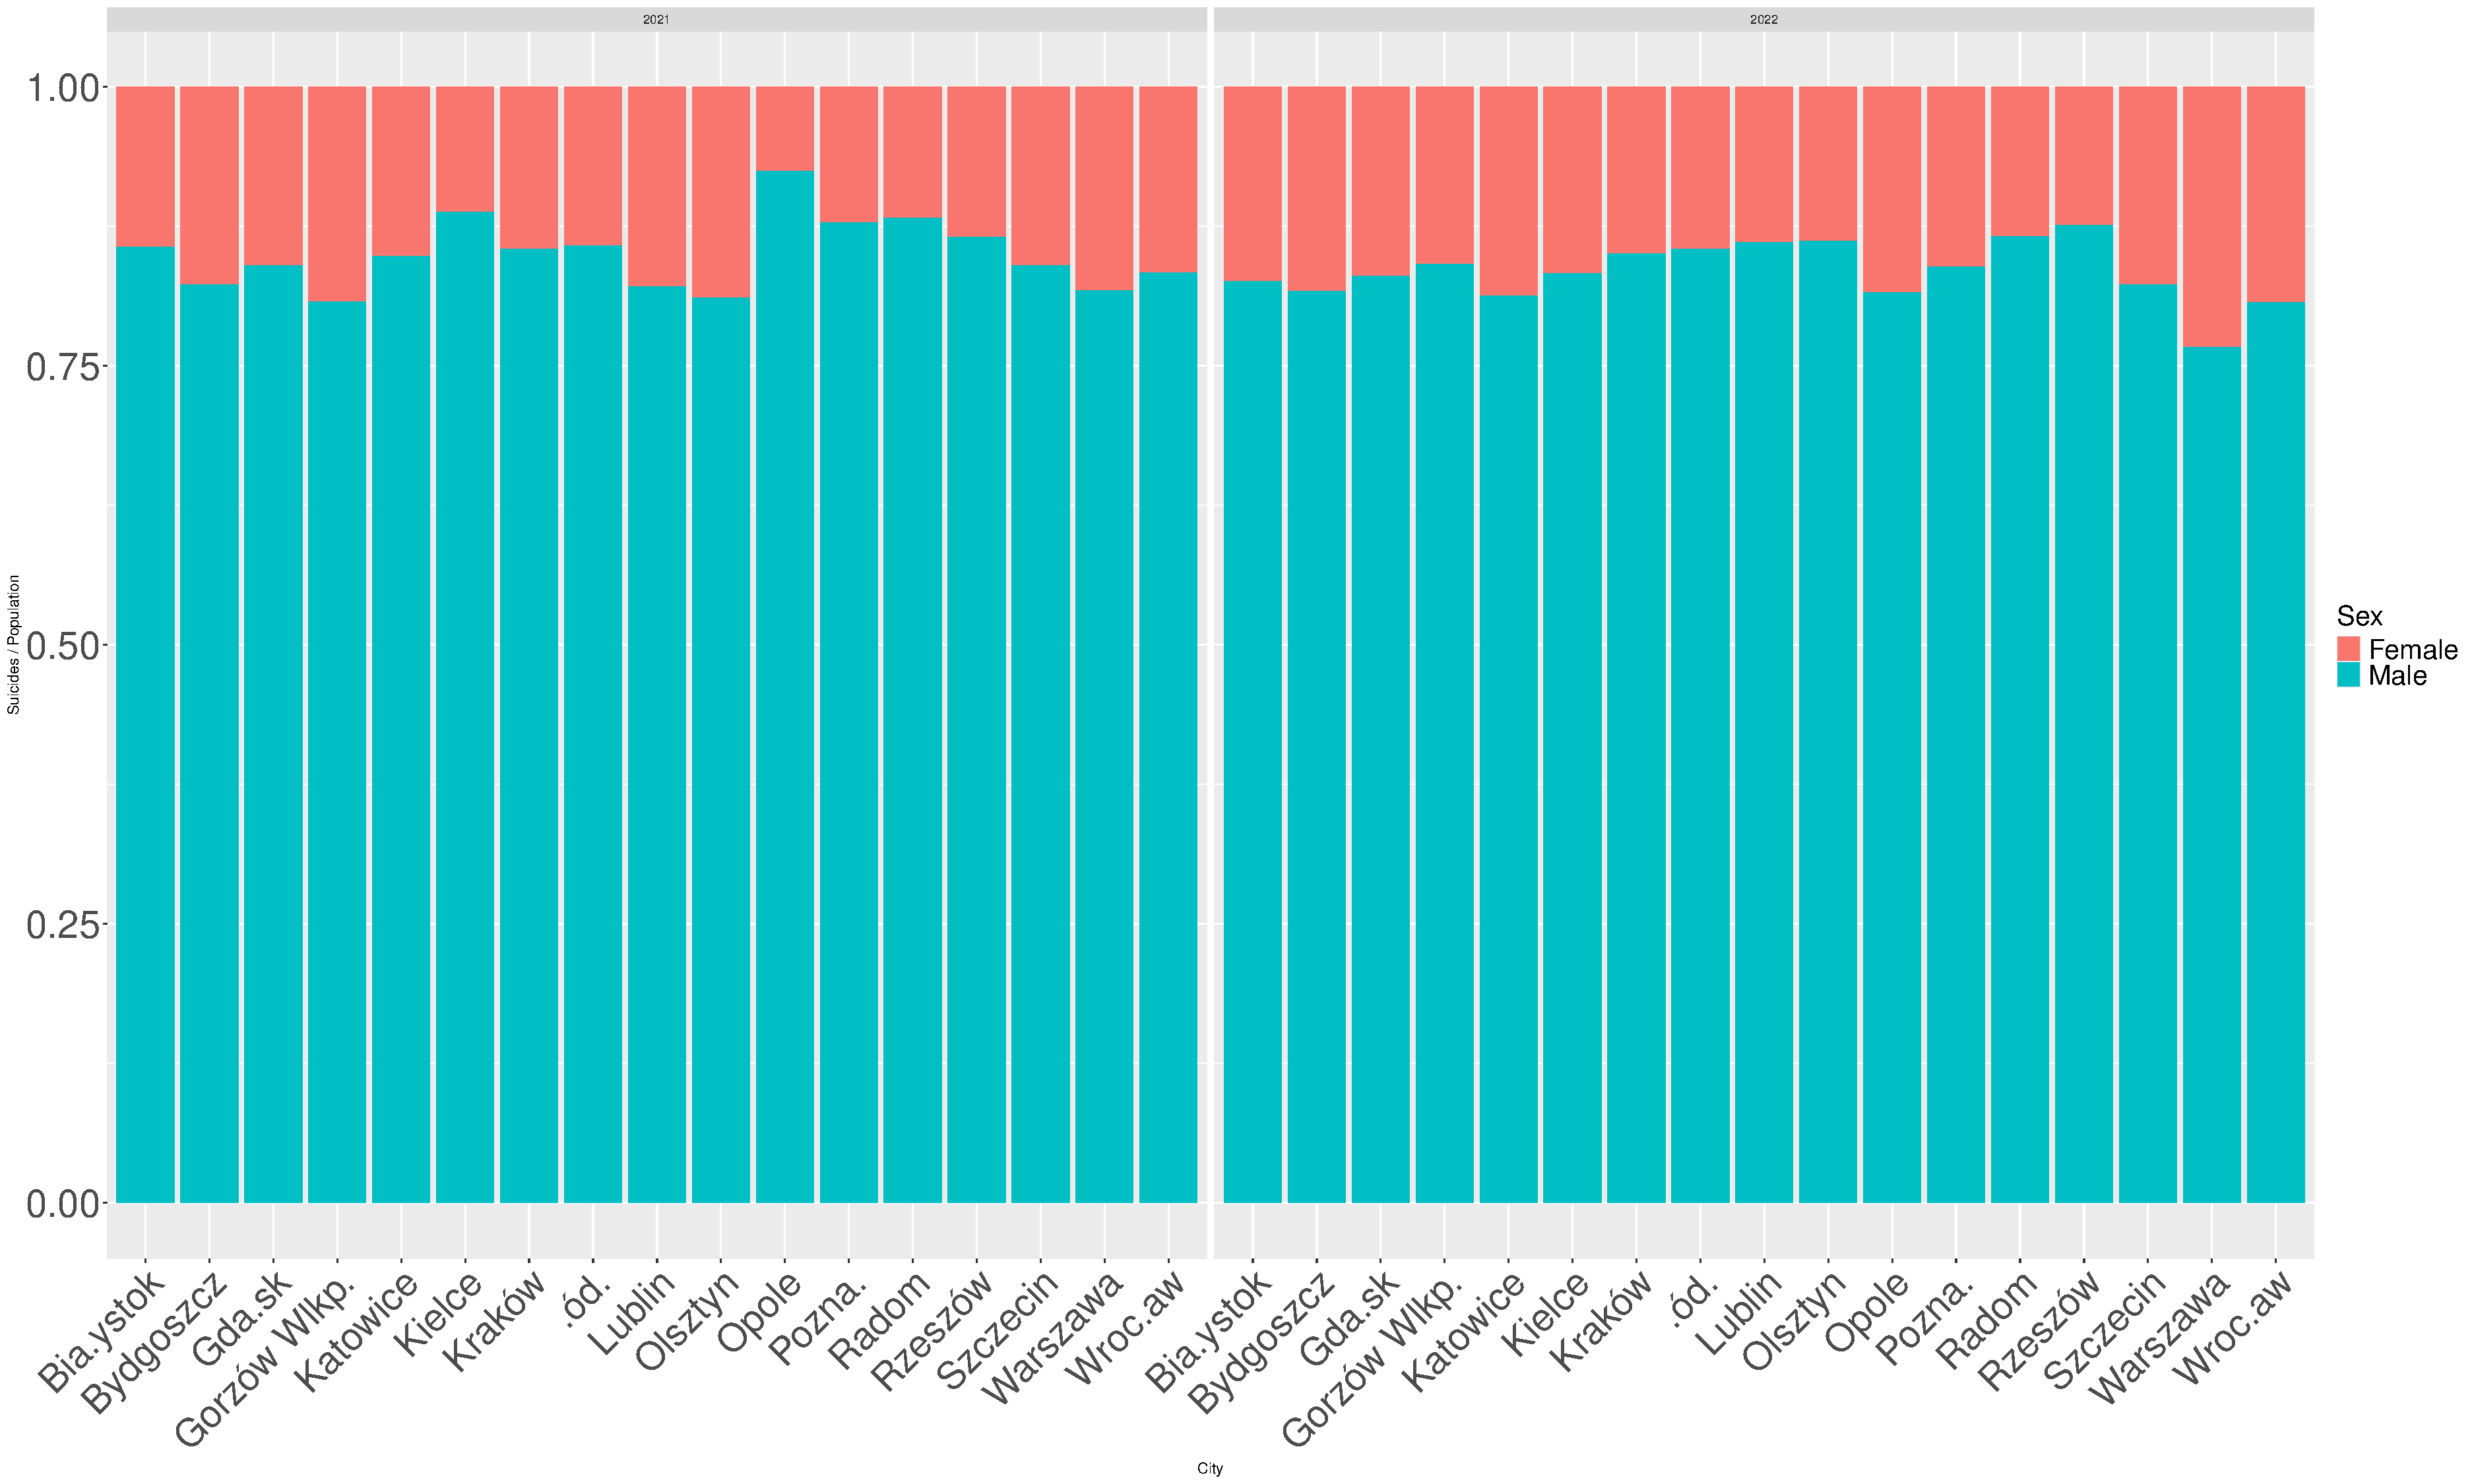
\includegraphics[width=0.65\textwidth]{imgs/sex_city_fat_suicides-2122.pdf}
    \caption{Fatal suicides by sex  in 2021 and 2022}
    \label{fig:sex_city_fat_suicides-2122}
\end{figure}

\begin{figure}[H]
    \centering
    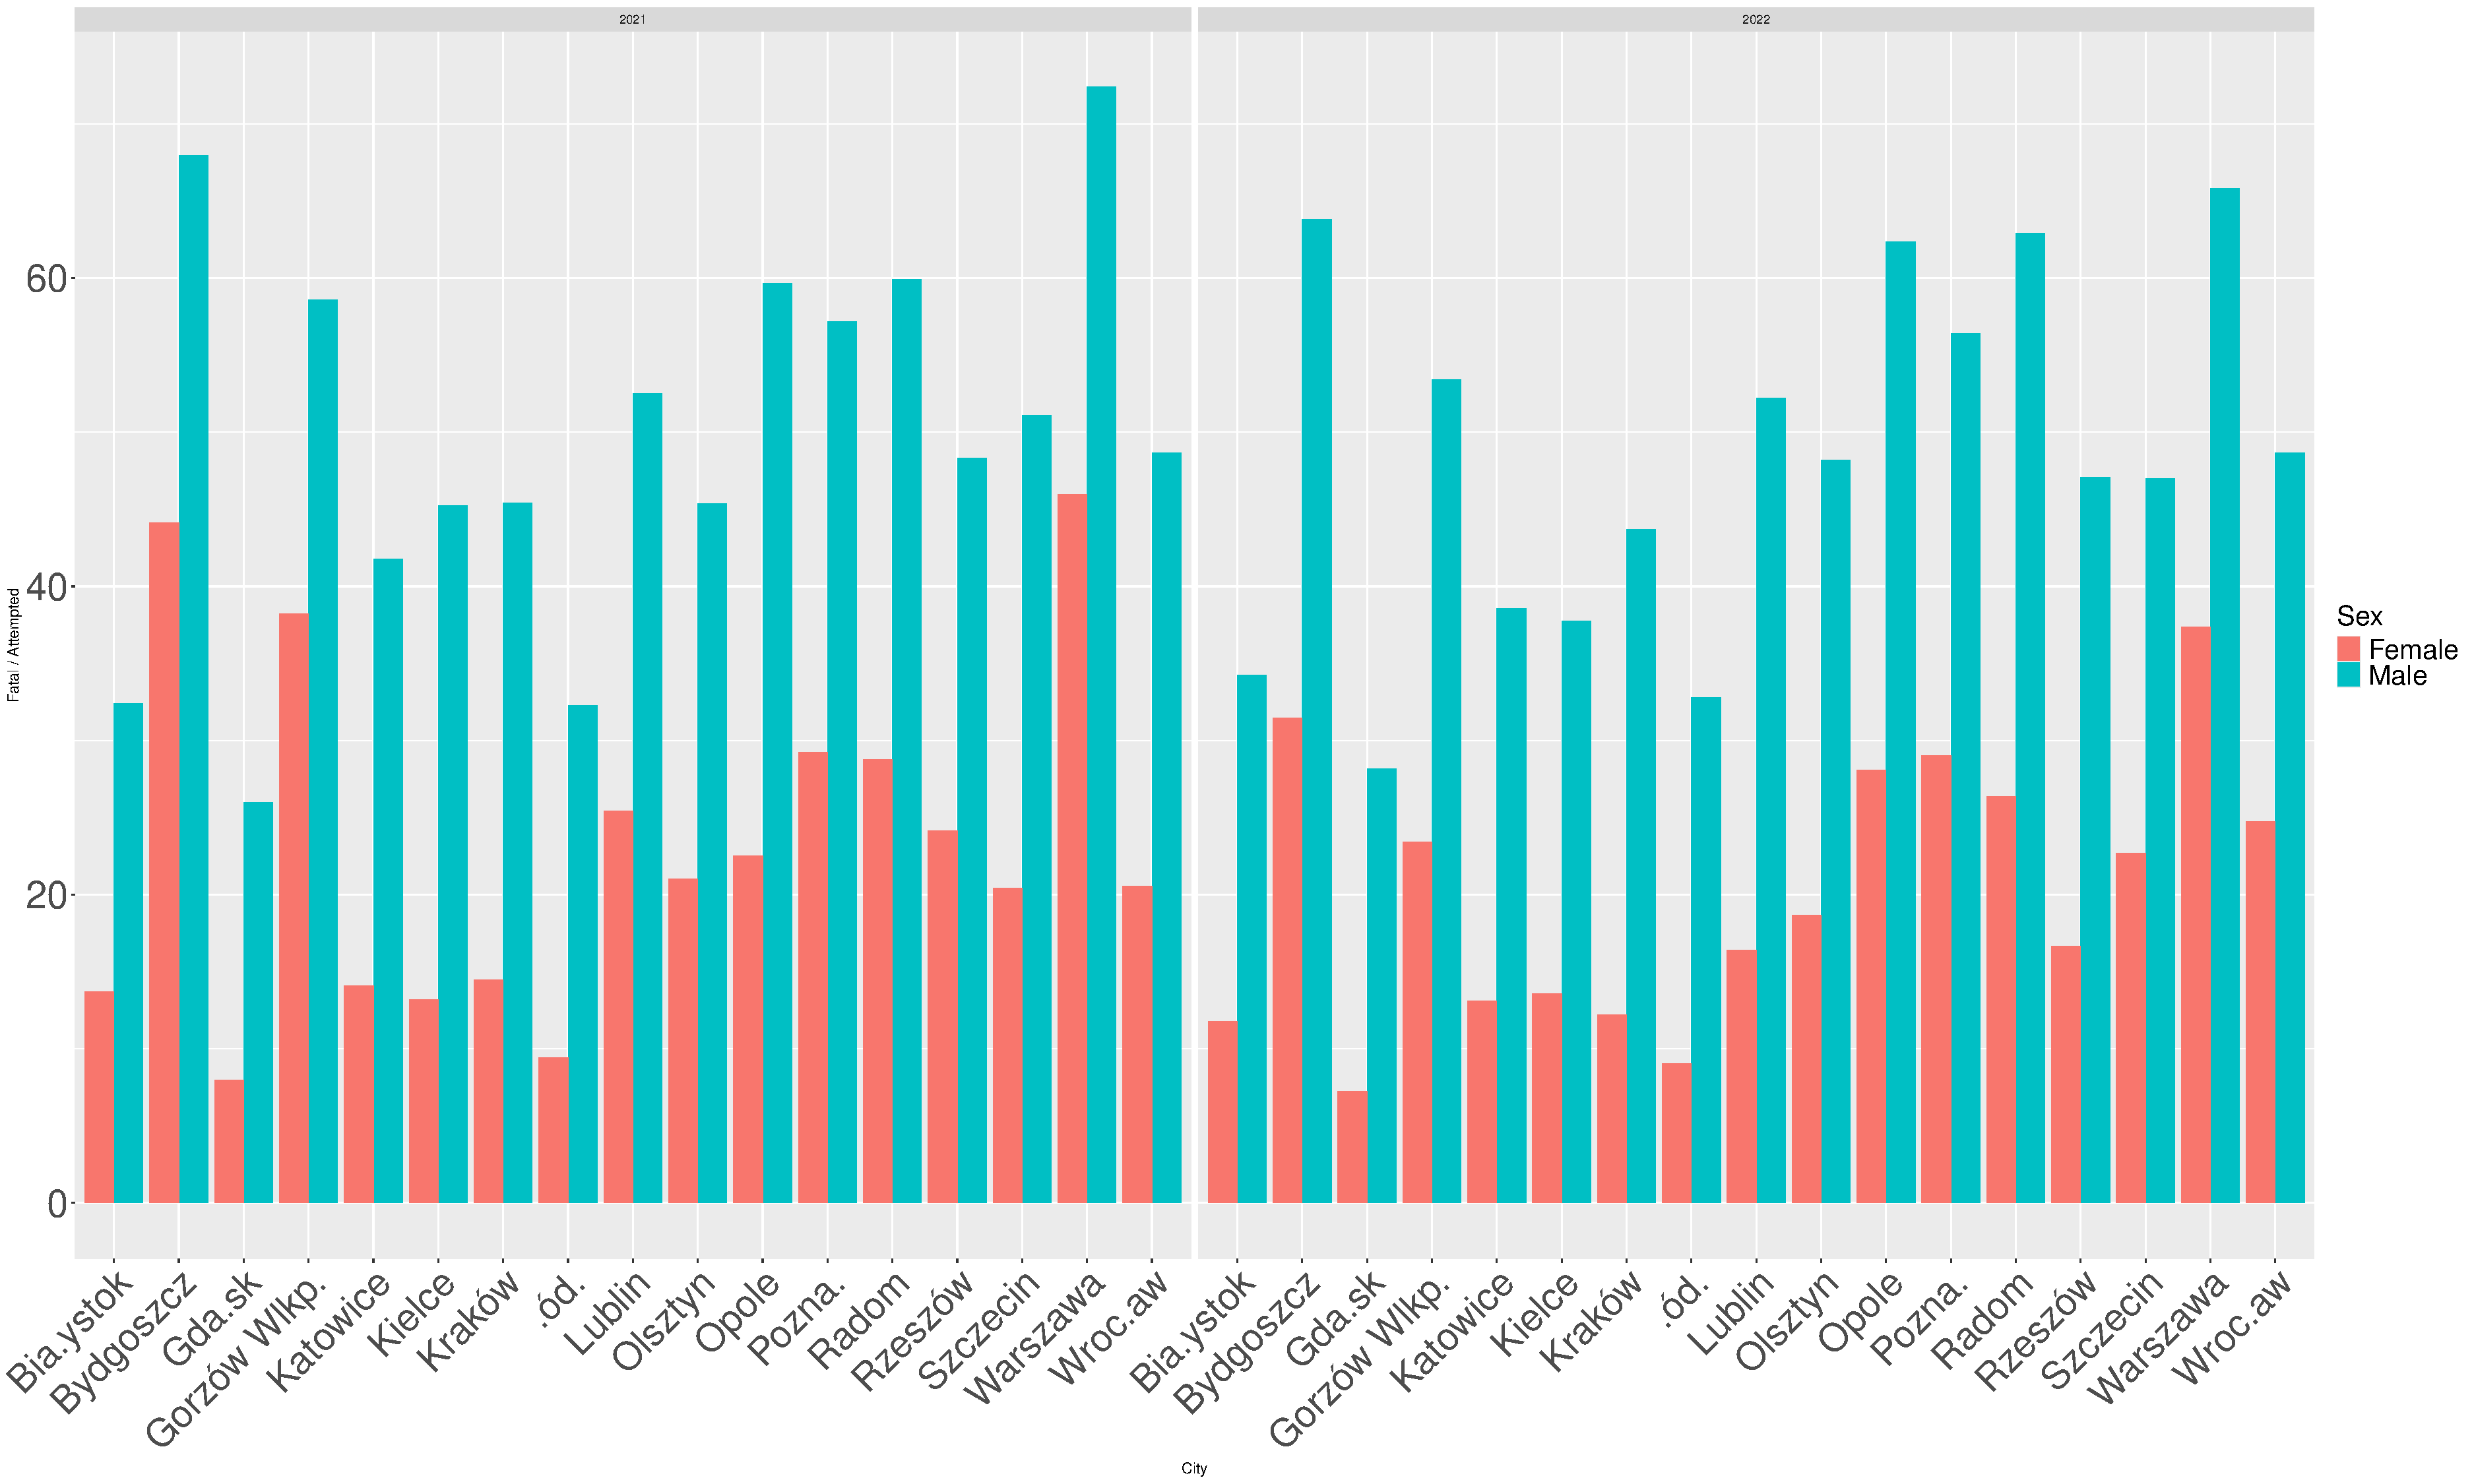
\includegraphics[width=0.65\textwidth]{imgs/sex_foa_city-2122.pdf}
    \caption{Fatal over attempted suicides by sex in different cities in 2021 and 2022}
    \label{fig:sex_foa_city-2122}
\end{figure}

%\begin{figure}[H]
%    \centering
%    \begin{minipage}{0.65\textwidth}
%        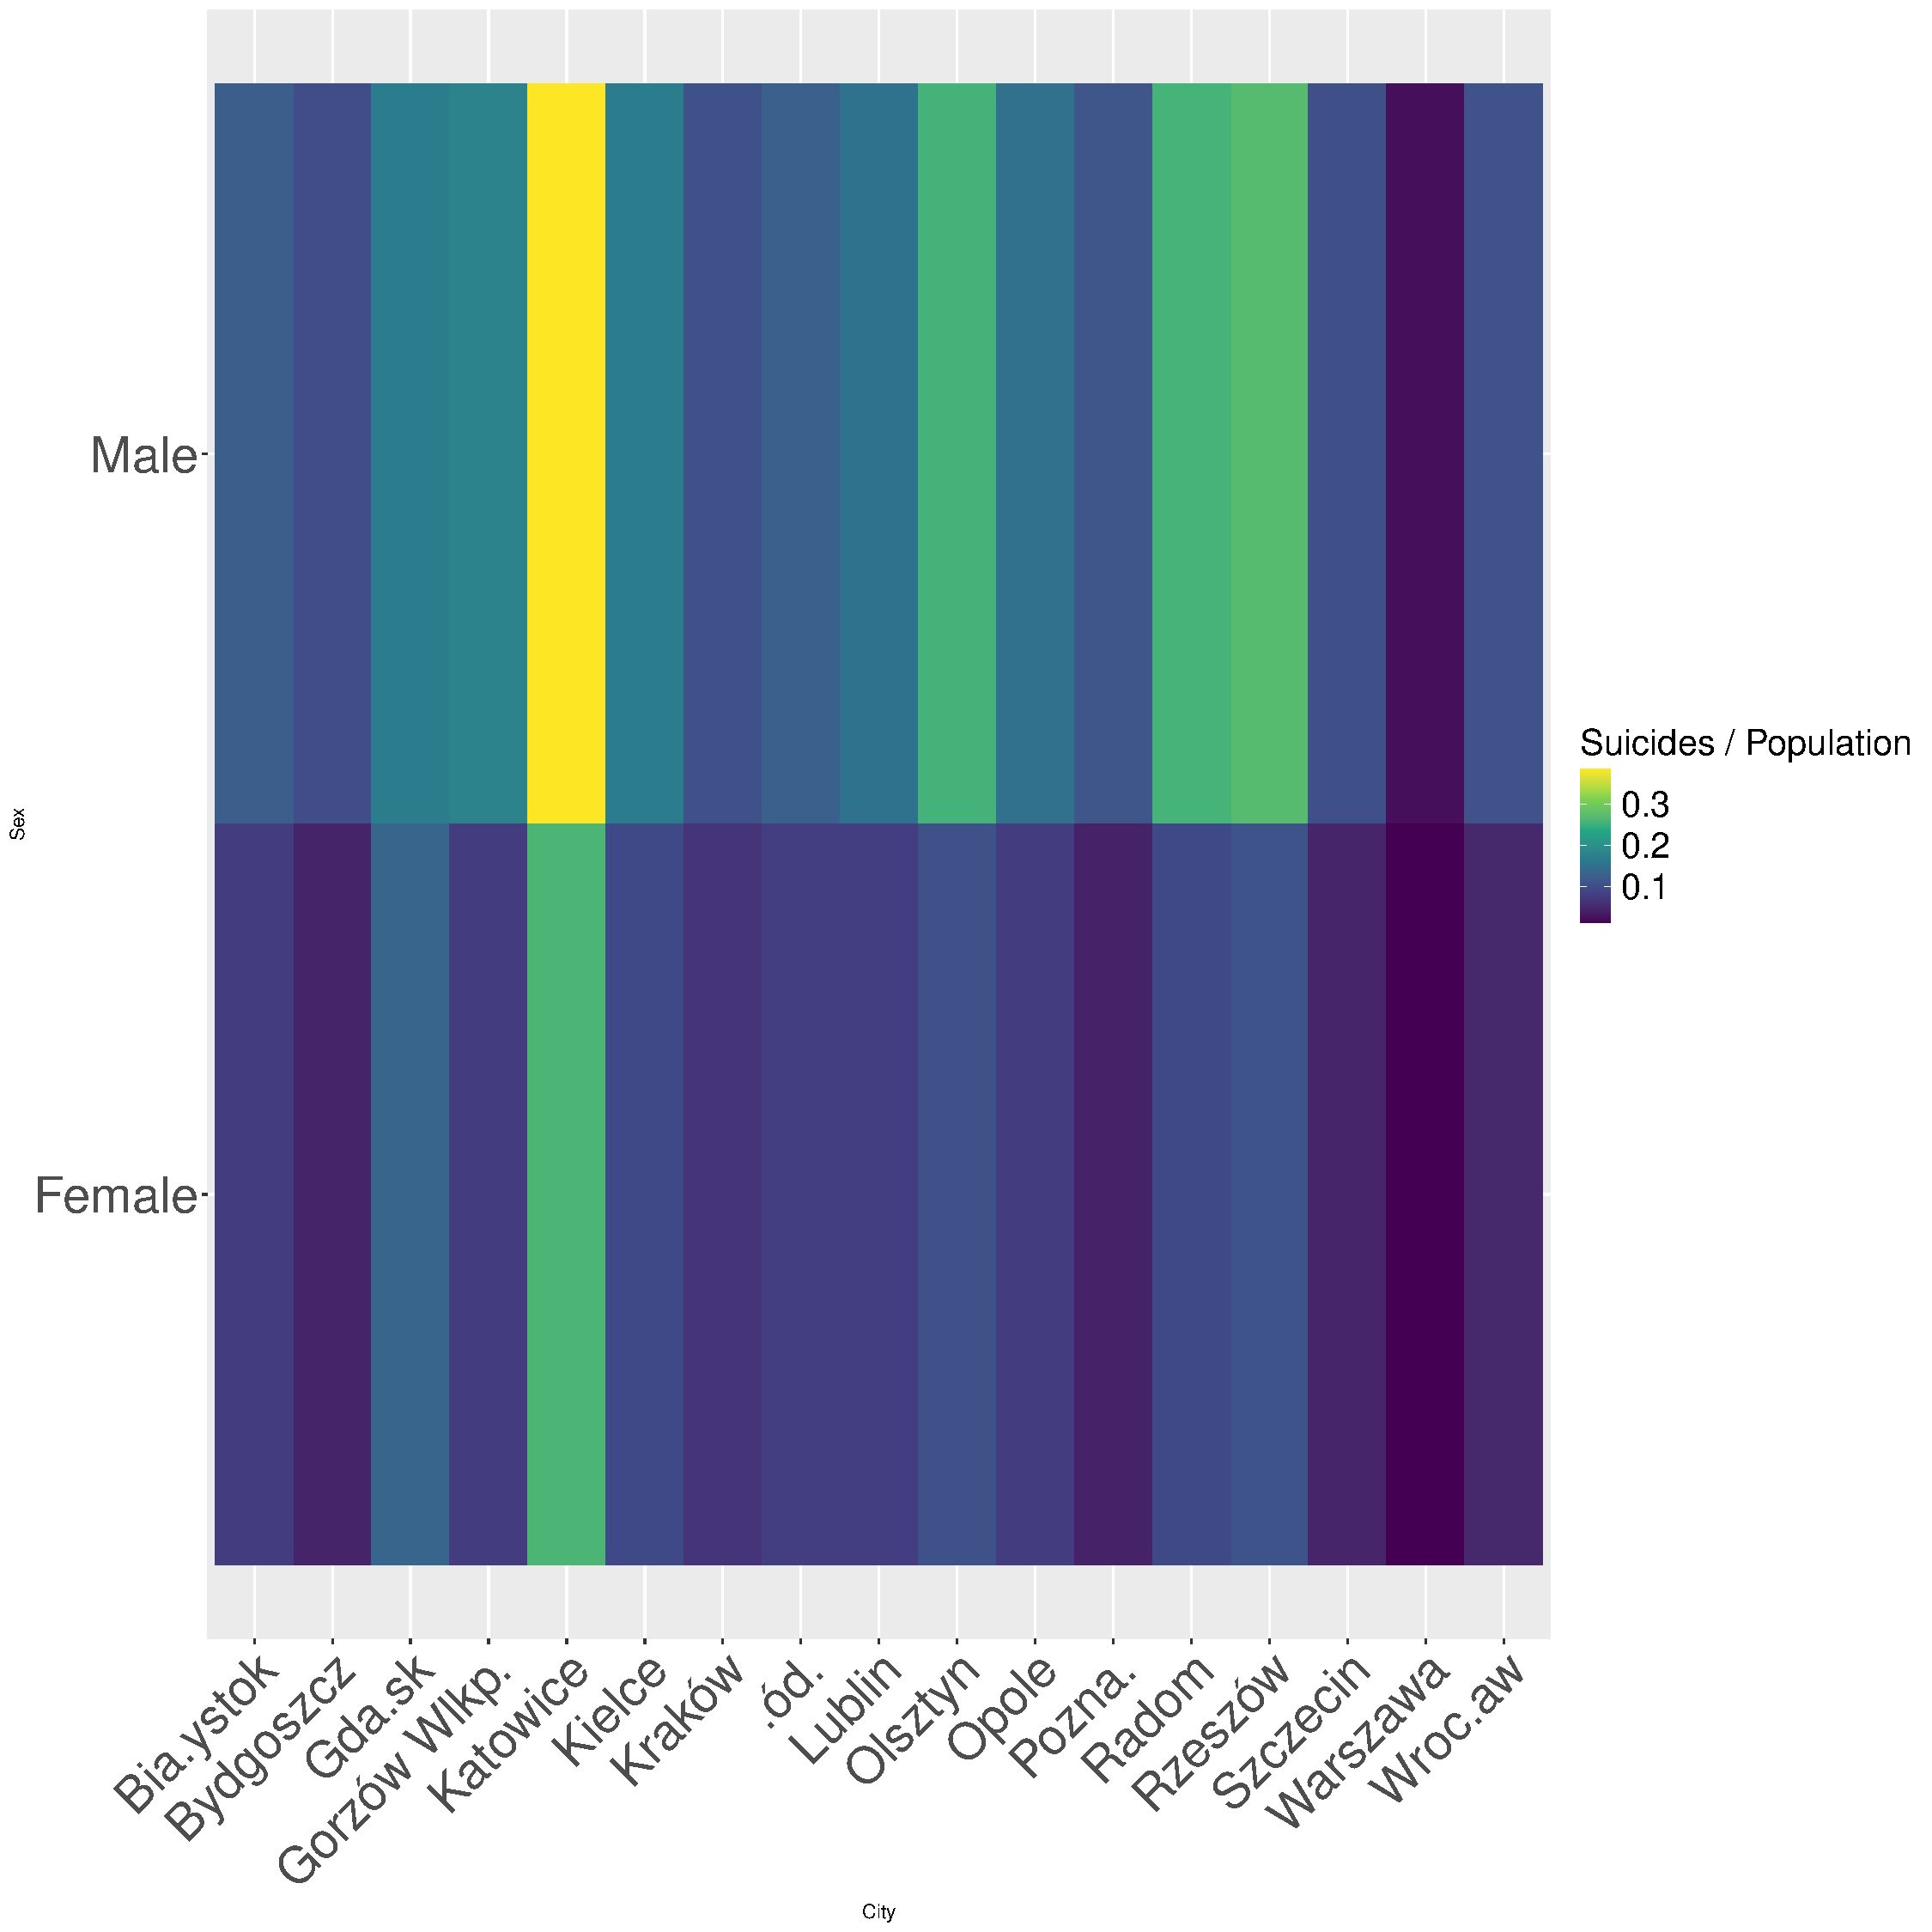
\includegraphics[width=\textwidth]{imgs/sex_city_op-att-2022.pdf}
%        \caption{Attempted suicides by sex  in 2022 in different cities}
%        \label{fig:sex_city_op-att-2022}
%    \end{minipage}
%    \hfill
%    \begin{minipage}{0.65\textwidth}
%        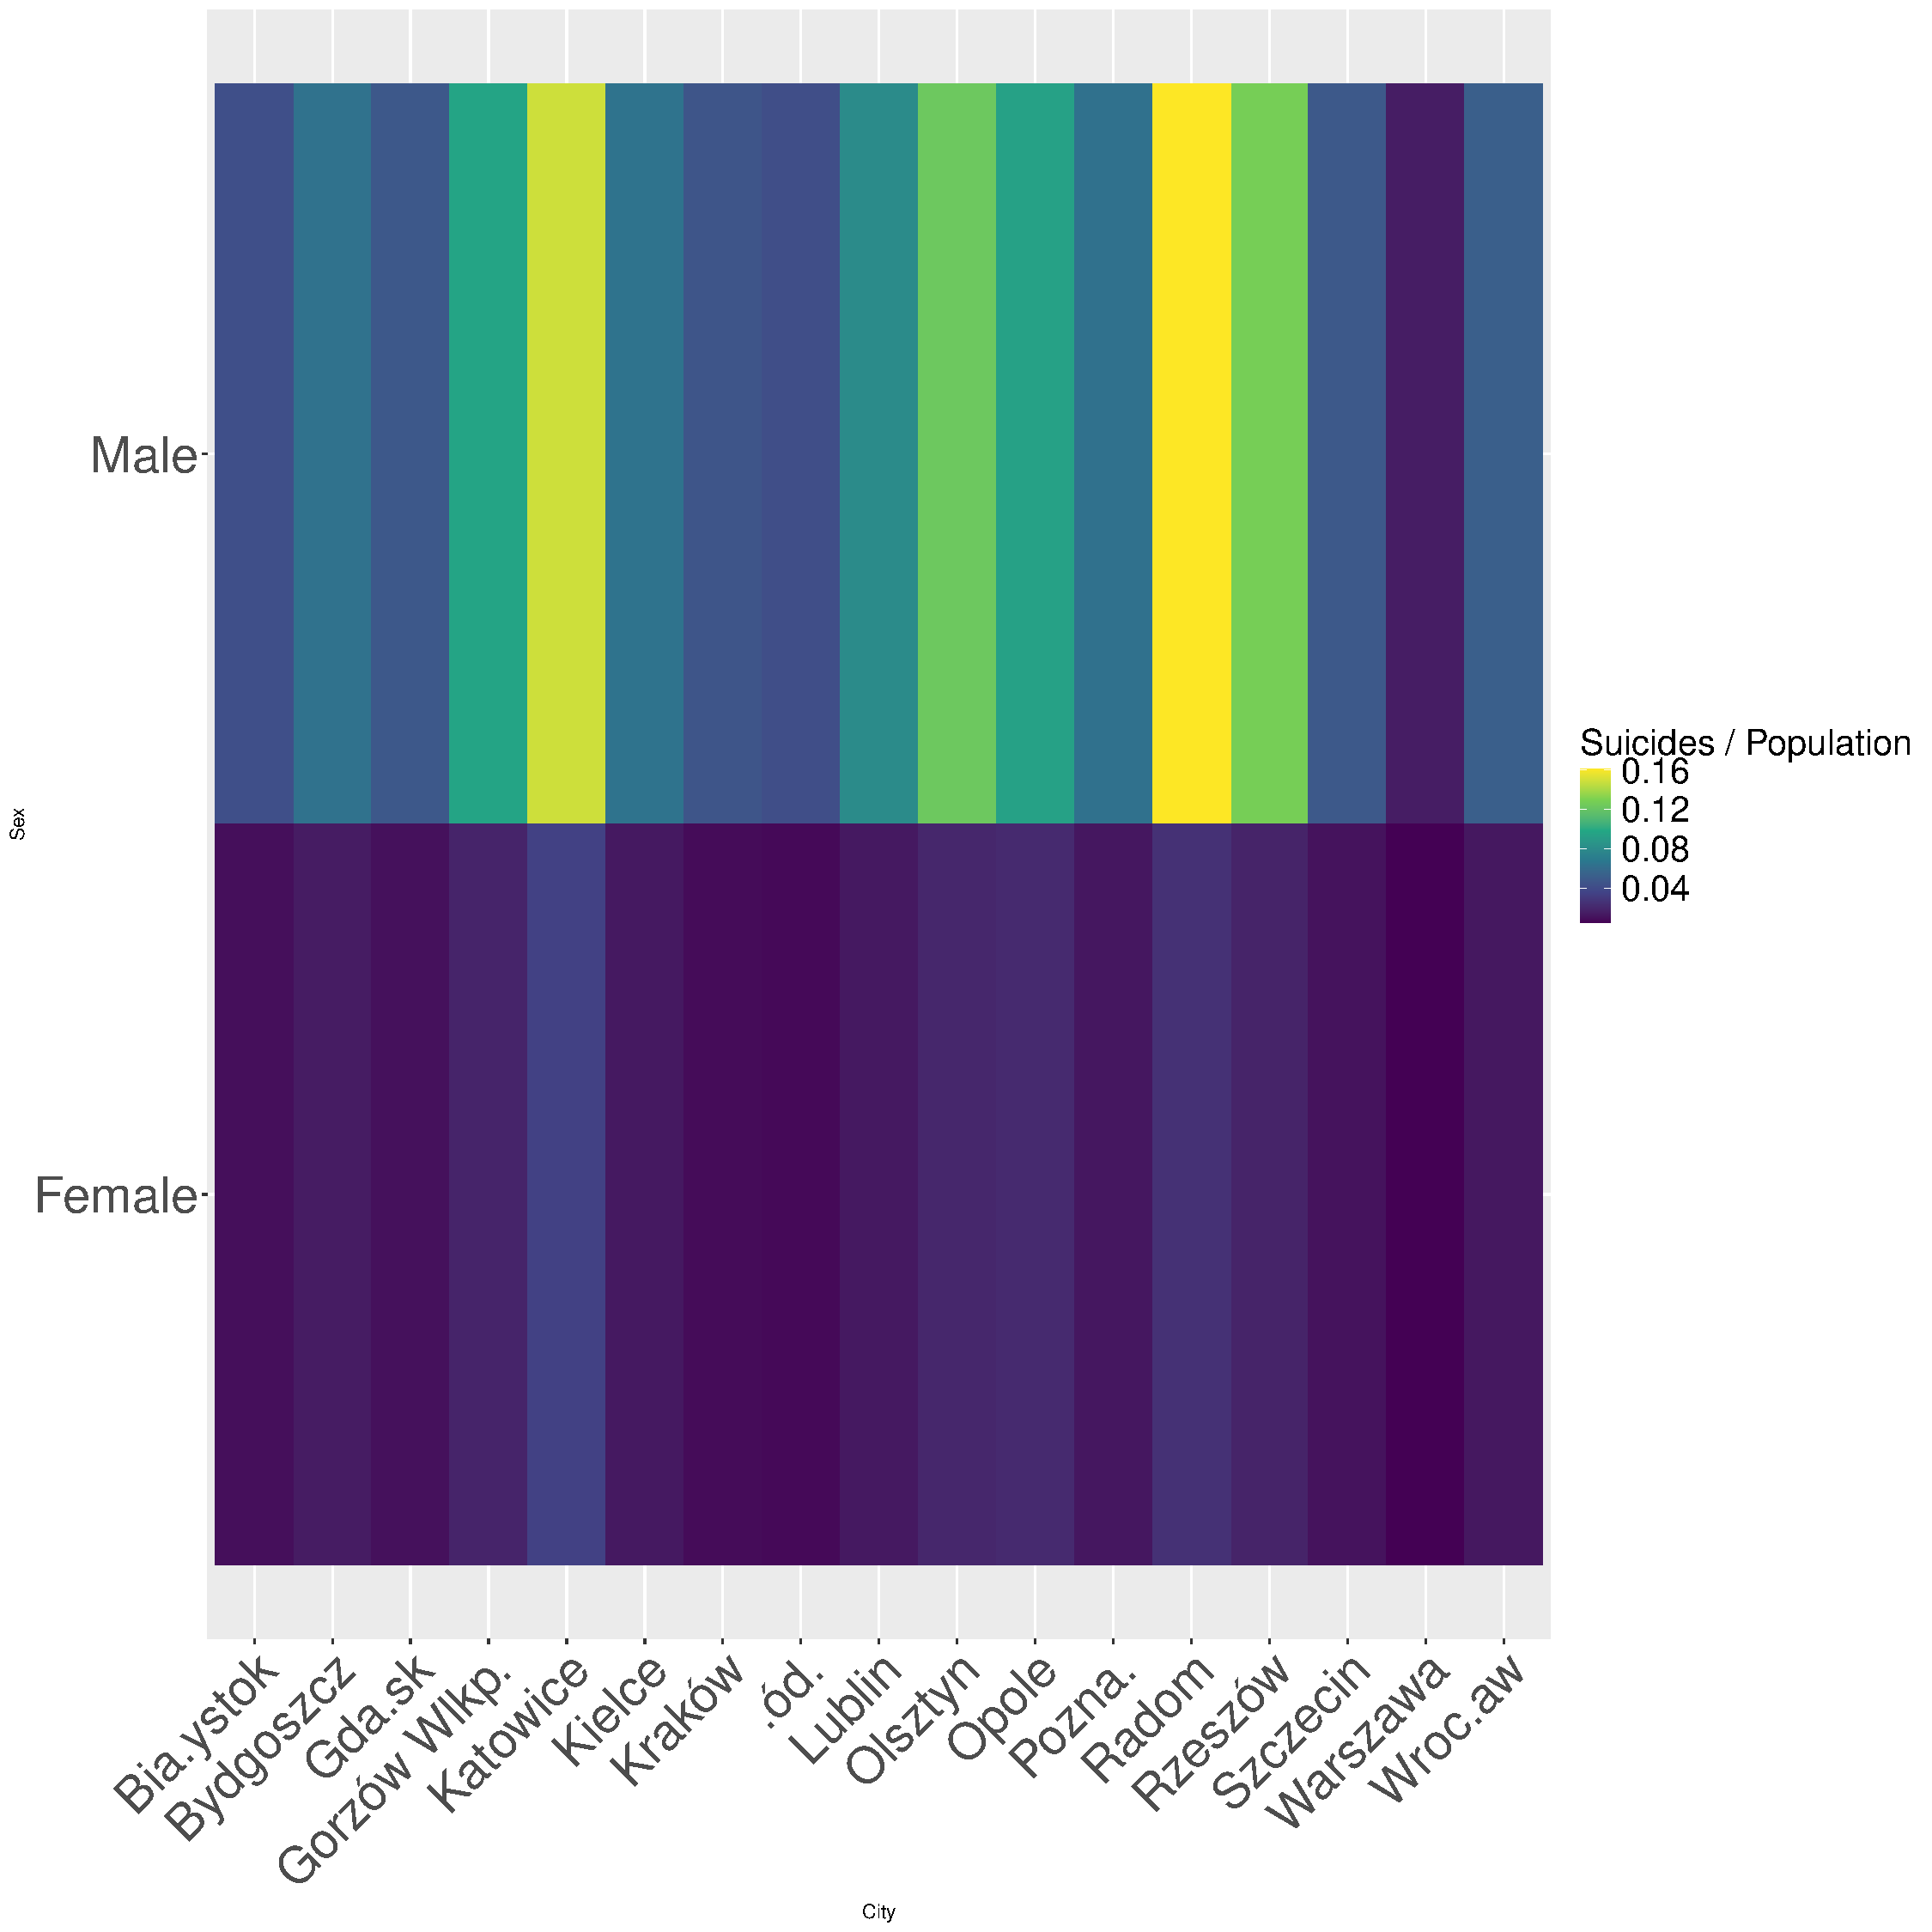
\includegraphics[width=\textwidth]{imgs/sex_city_op-fat-2022.pdf}
%        \caption{Fatal suicides by sex  in 2022 in different cities}
%        \label{fig:sex_city_op-fat-2022}
%    \end{minipage}
%\end{figure}
%



%
%
\subsection{Place}
%
%
Figures \ref{fig:place_attempted}, \ref{fig:place_fatal}, \ref{fig:place_foa},
reveal that the most common place where people in Poland attempt suicide is 
home, then other common places are farms, basements and forests,
suicides committed in farms decreased in time, whereas suicides at home,
on the street and on railways increased.
The places where most suicide attempts resulted fatal were farms,
basements, forests and legal isolations.
%
%
\begin{figure}[H]
    \centering
    \begin{minipage}{0.65\textwidth}
        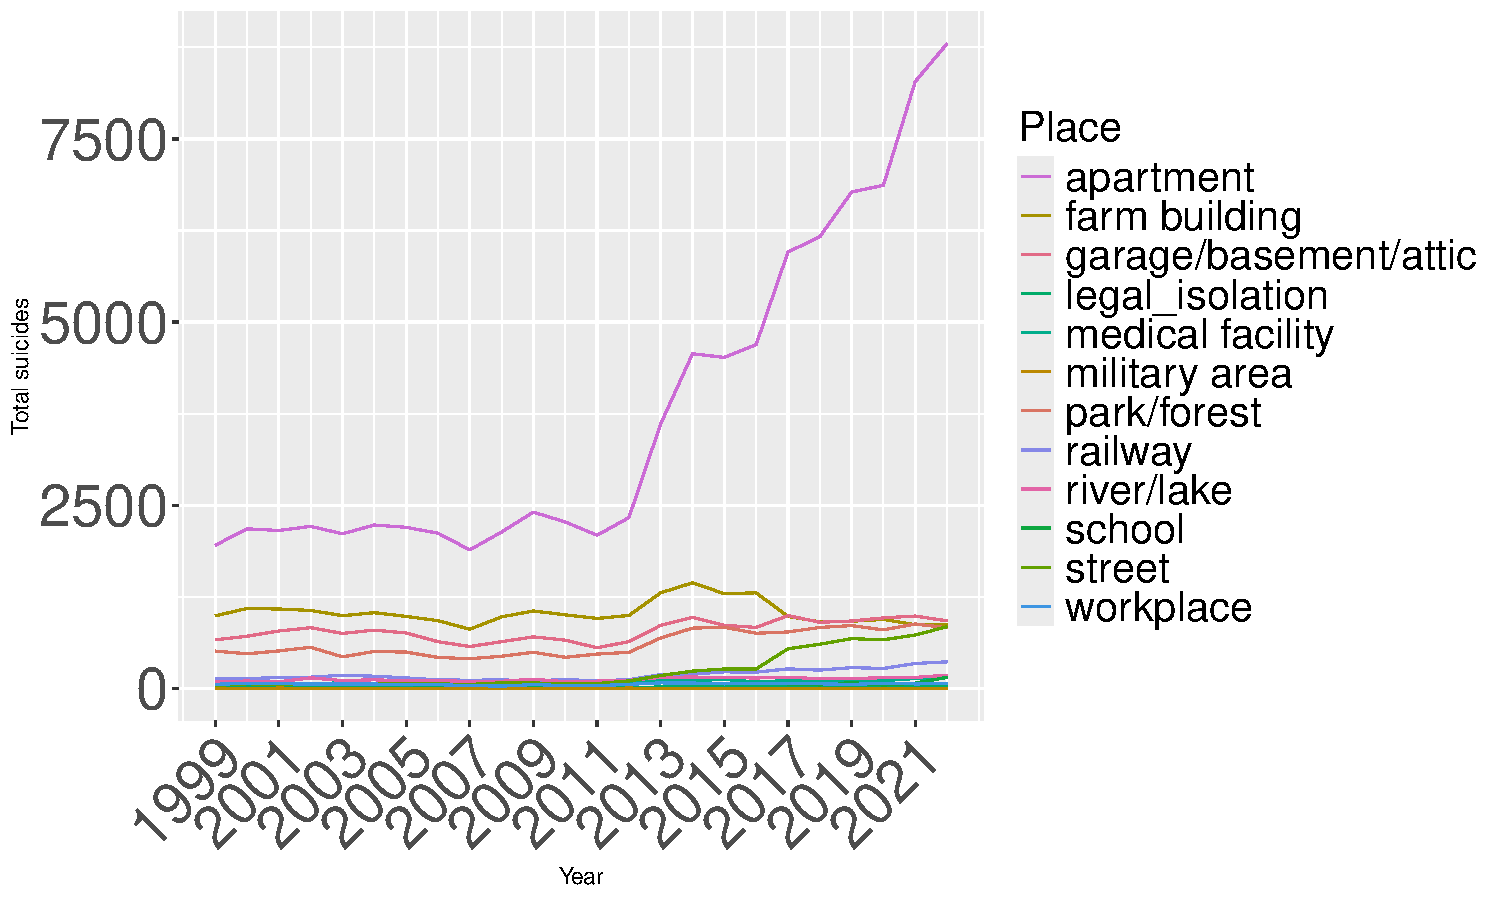
\includegraphics[width=\textwidth]{imgs/place_attempted.pdf}
        \caption{Trend of attempted suicides by place }
	\label{fig:place_attempted}
    \end{minipage}
    \hfill
    \begin{minipage}{0.65\textwidth}
        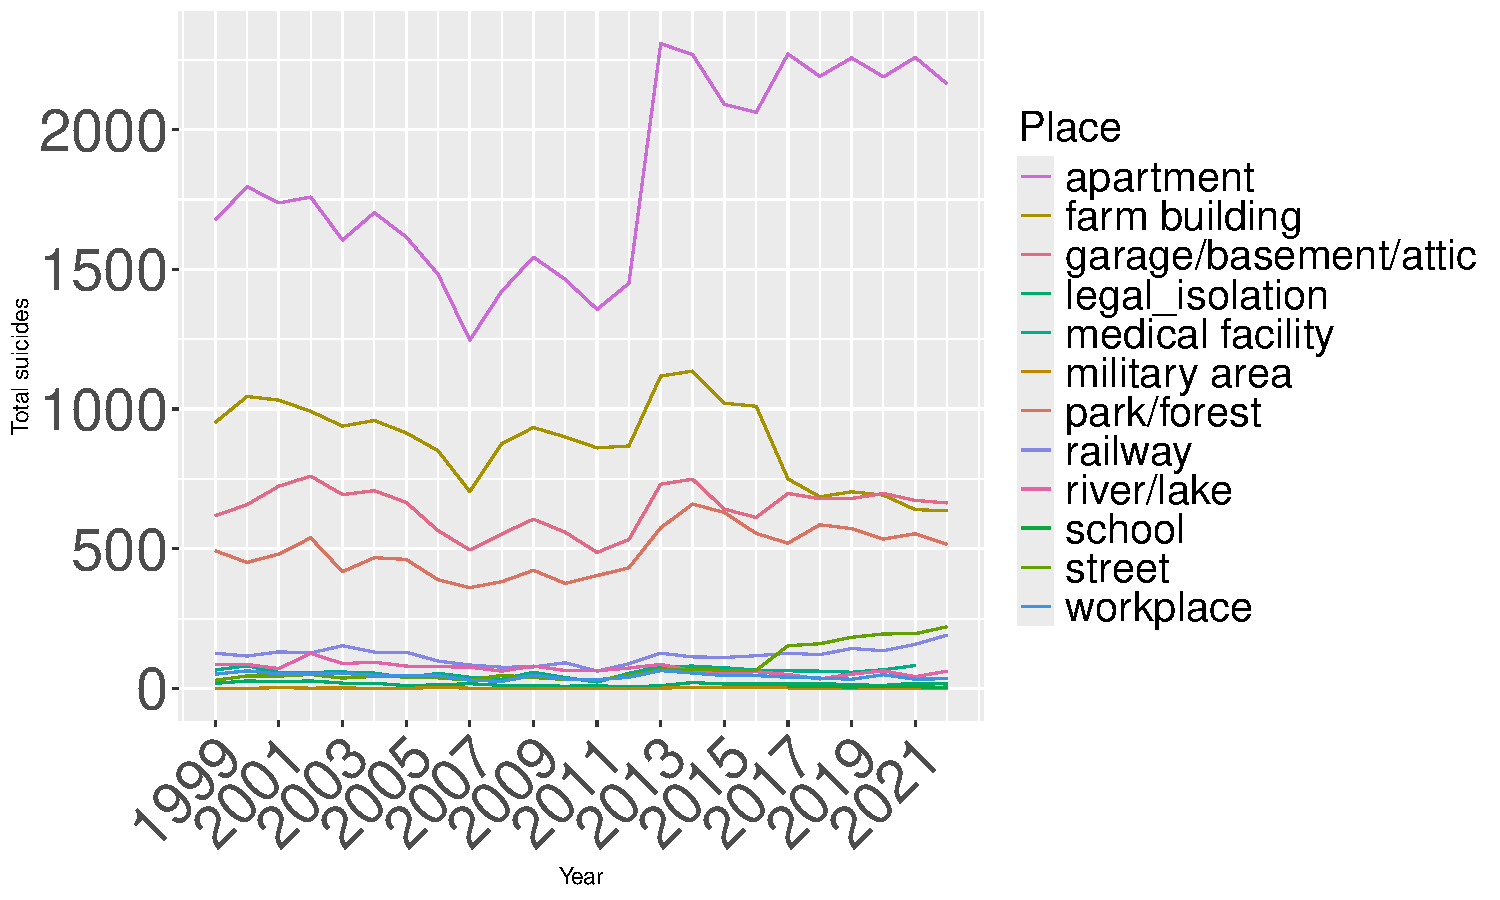
\includegraphics[width=\textwidth]{imgs/place_fatal.pdf}
        \caption{Trend of fatal suicides by place }
	\label{fig:place_fatal}
    \end{minipage}
\end{figure}

\begin{figure}[H]
    \centering
    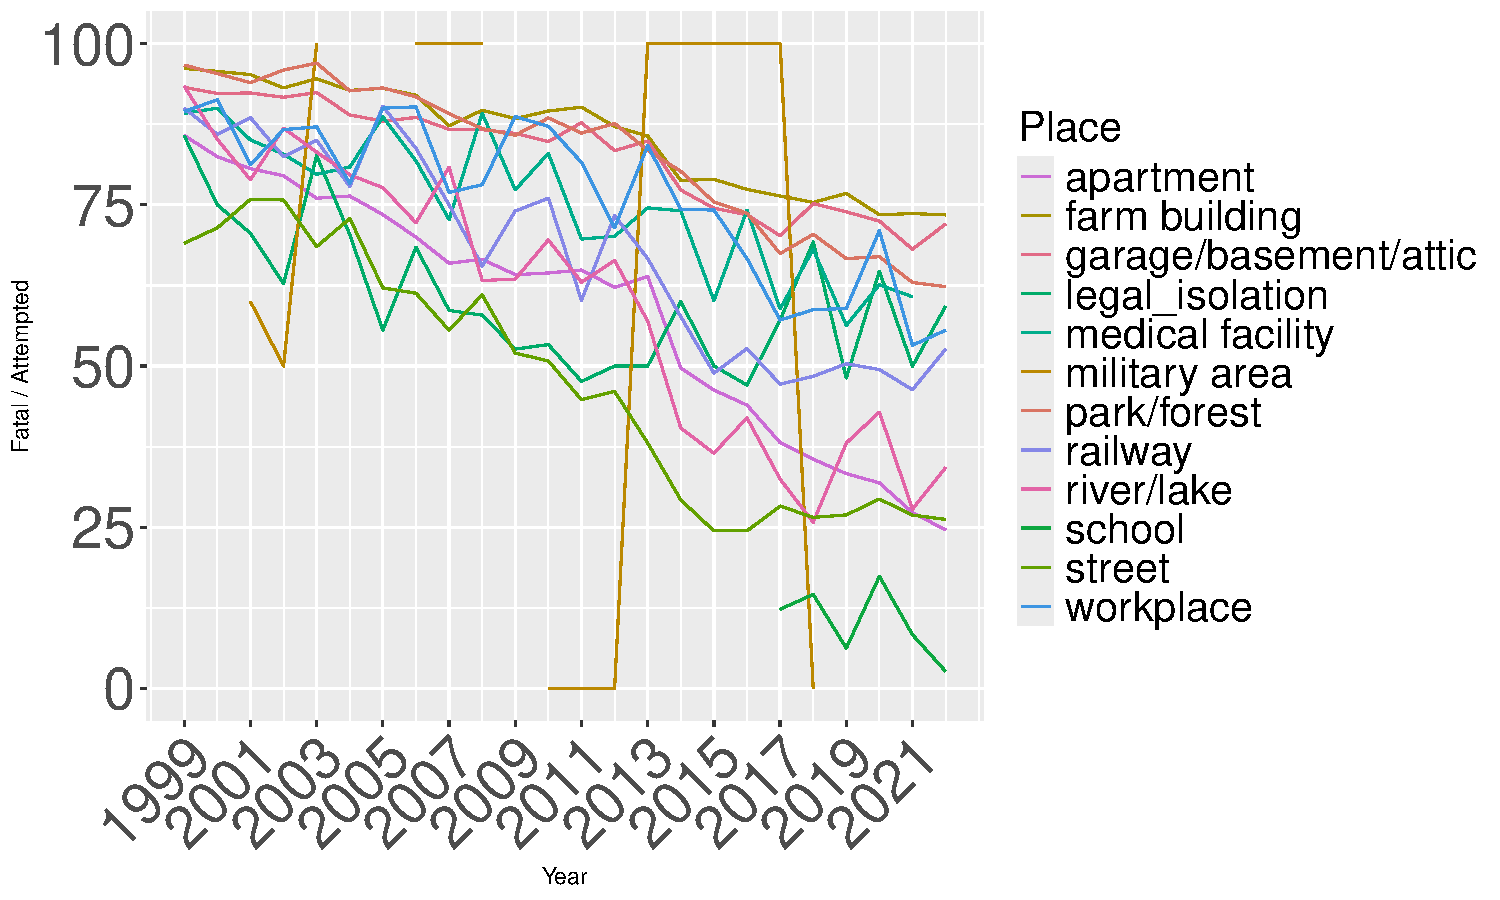
\includegraphics[width=0.65\textwidth]{imgs/place_foa.pdf}
    \caption{Trend of fatal over attempted suicides by place }
    \label{fig:place_foa}
\end{figure}
%
%
The heatmap in figure \ref{fig:place_foa_heat} confirms that 
suicide attempts inside farms, basements and forests kept a higher fatal outcome
rate whereas those in the apartment decreased during the years, suicide attempts in schools
have been documented only since 2017 and fortunately they often did not result in death.
The row relative to military areas shows abrupt gradients because of the small number of cases,
the only time when more than 2 attempts of suicide happened was in 2012 in Lublin (3 attempts, 0 resulted
in death).
%
%
\begin{figure}[H]
    \centering
    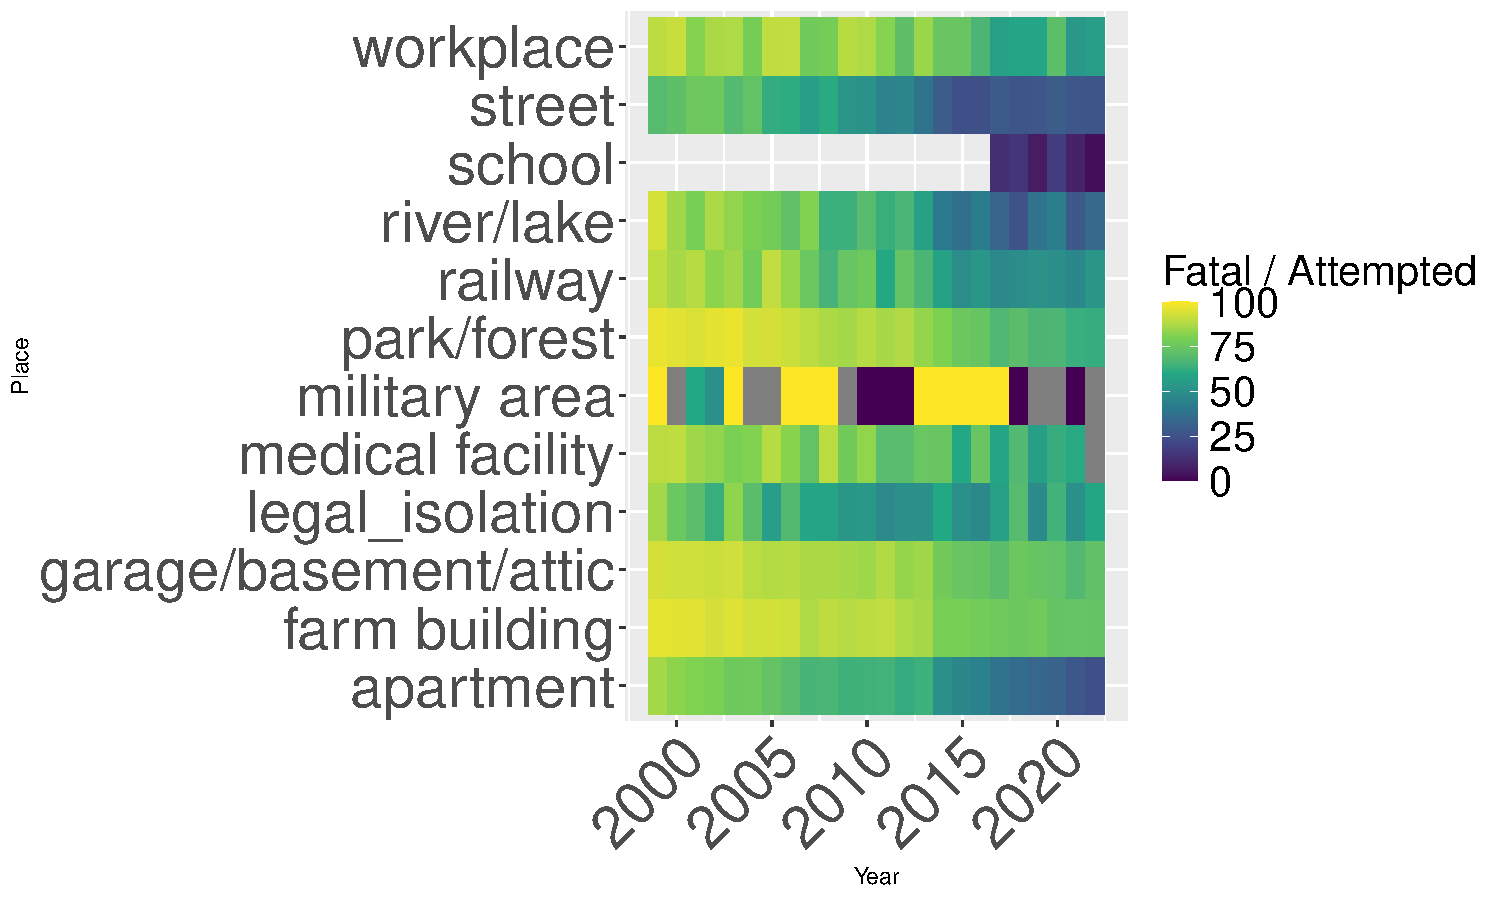
\includegraphics[width=0.65\textwidth]{imgs/place_foa_heat.pdf}
    \caption{Heatmap of fatal over attempted suicides by place }
    \label{fig:place_foa_heat}
\end{figure}
%
%
The barplots in \ref{fig:place_city_att_suicides-991020}
do not reveal particular differences among different cities,
and neither do those in \ref{fig:place_city_att_suicides-2122},
barplots in \ref{fig:place_city_fat_suicides-991020} and \ref{fig:place_city_fat_suicides-2122}
confirm that among suicides resulting in a fatal outcome those committed in the apartment
are less predominant than they are when considering suicide attempts in general.
\begin{figure}[H]
    \centering
    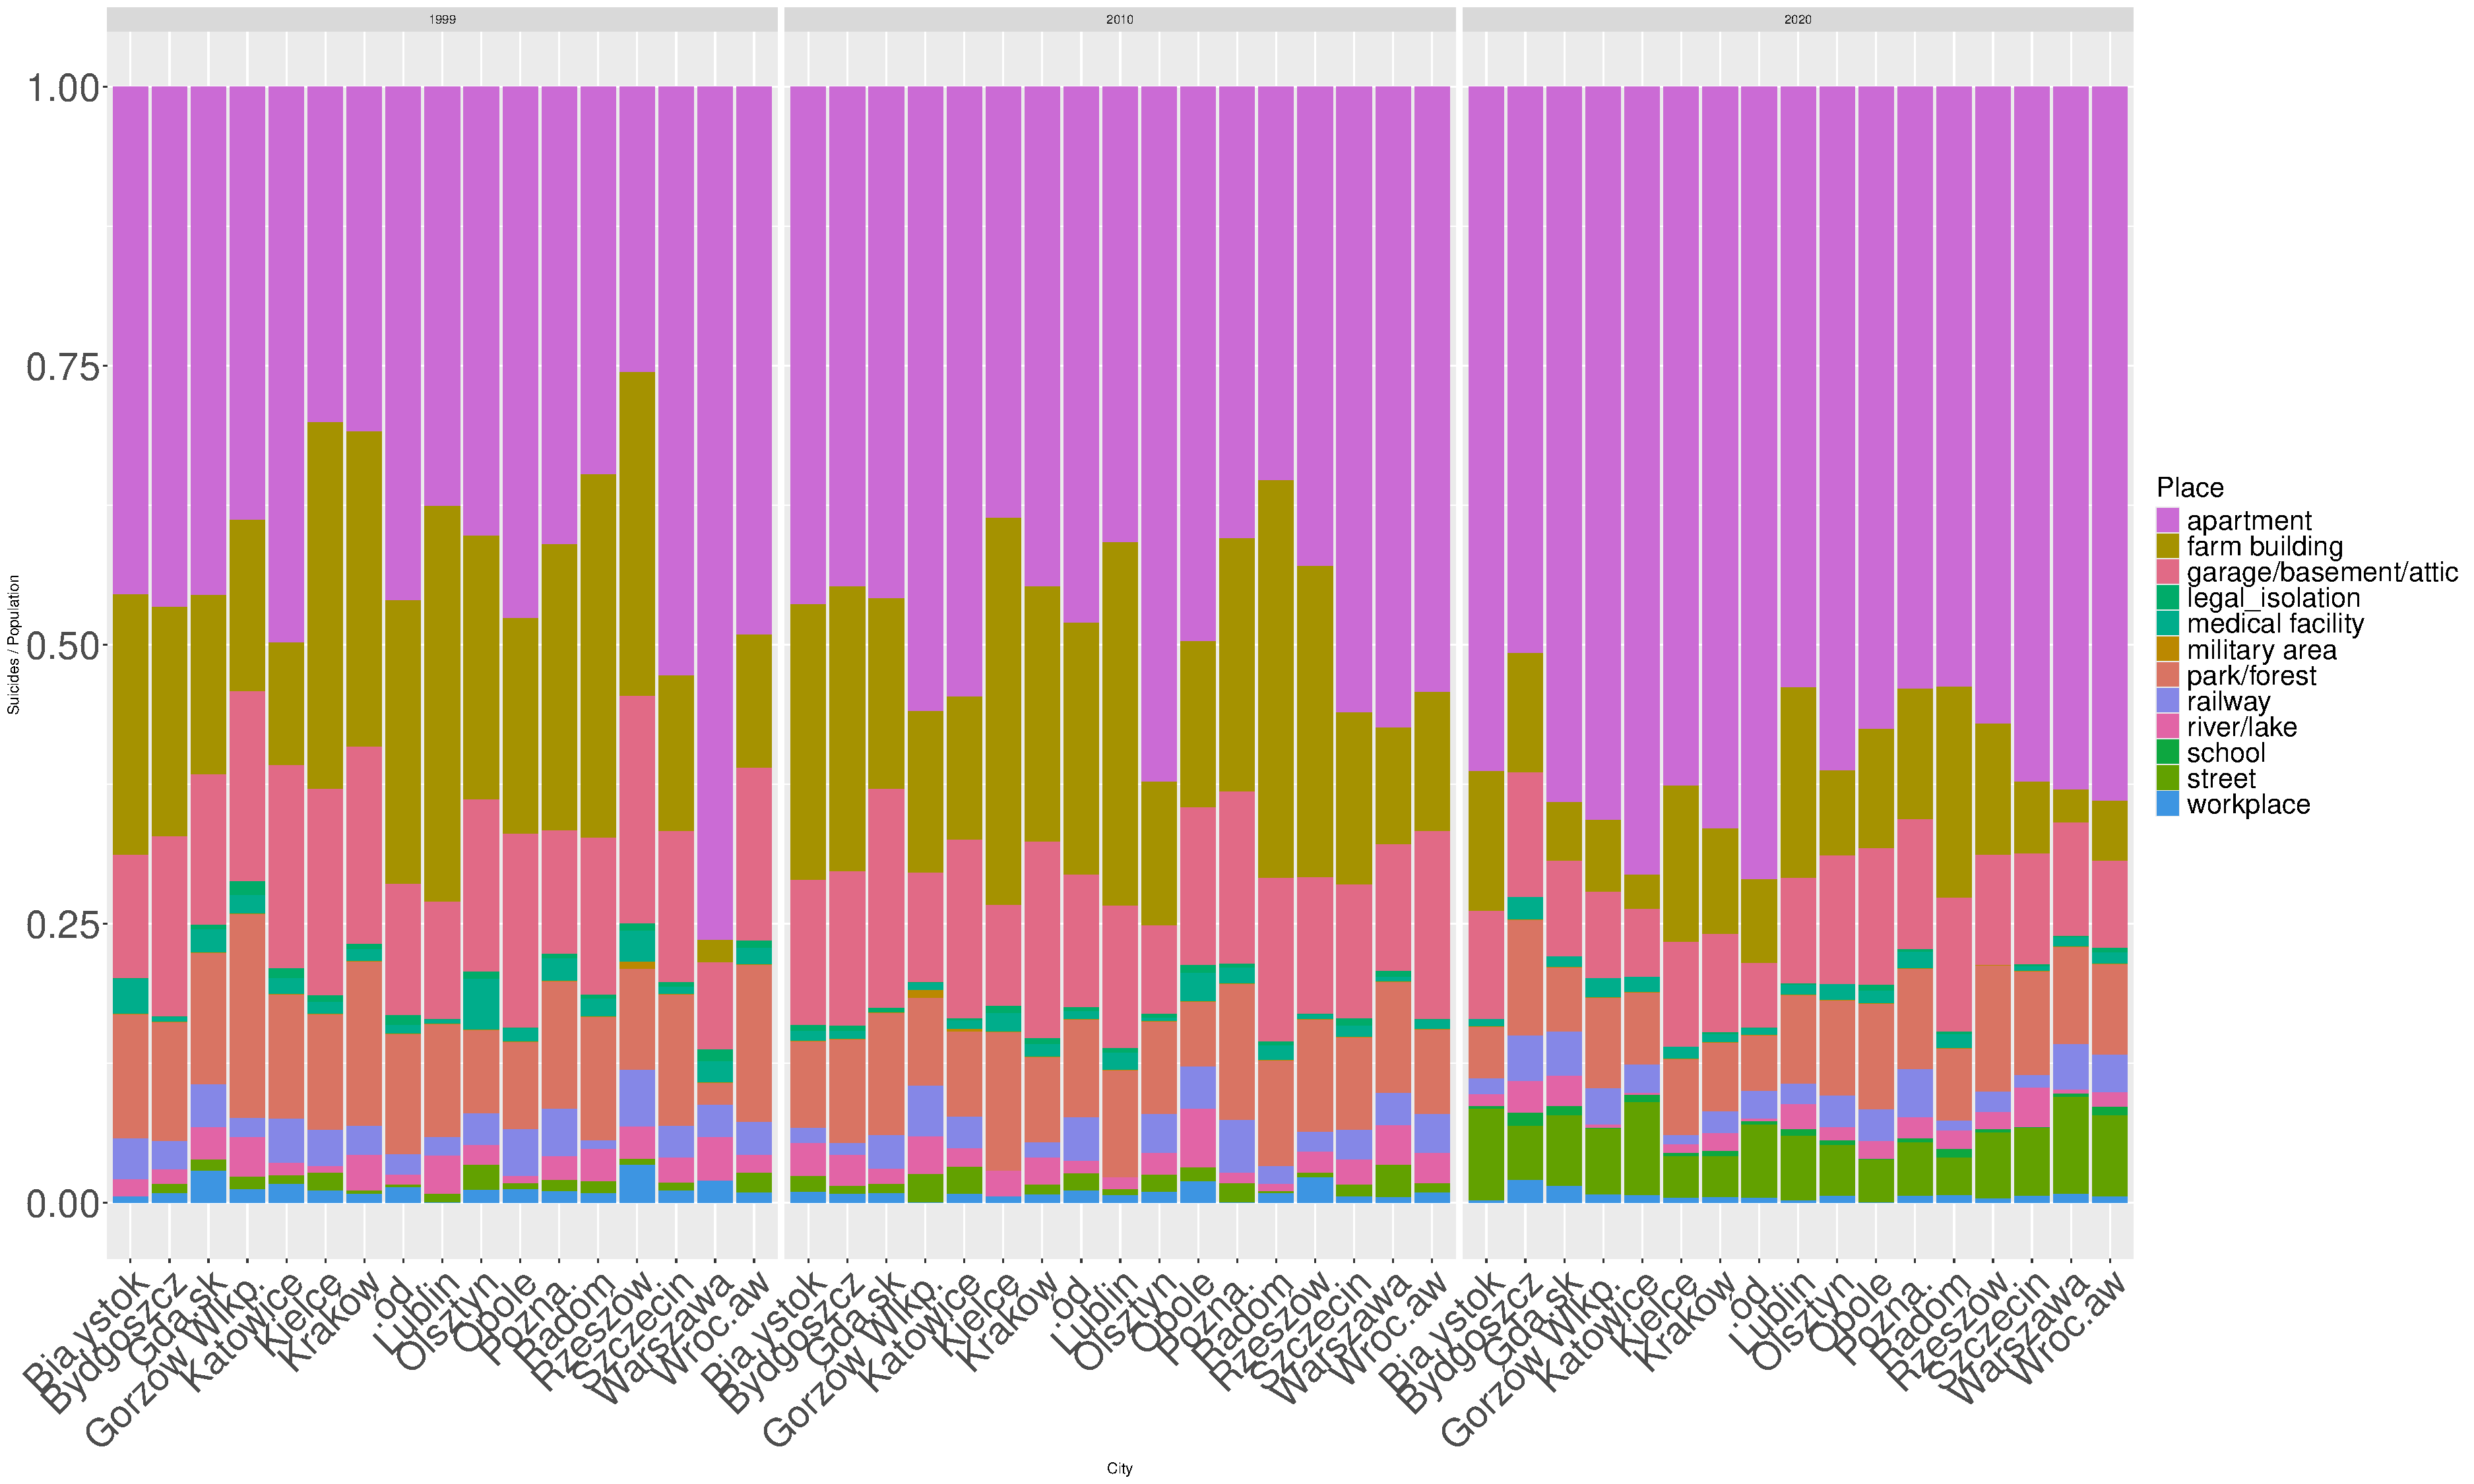
\includegraphics[width=0.65\textwidth]{imgs/place_city_att_suicides-991020.pdf}
    \caption{Attempted suicides by place in different cities in 1999, 2010 and 2020}
    \label{fig:place_city_att_suicides-991020}
\end{figure}
%
\begin{figure}[H]
    \centering
    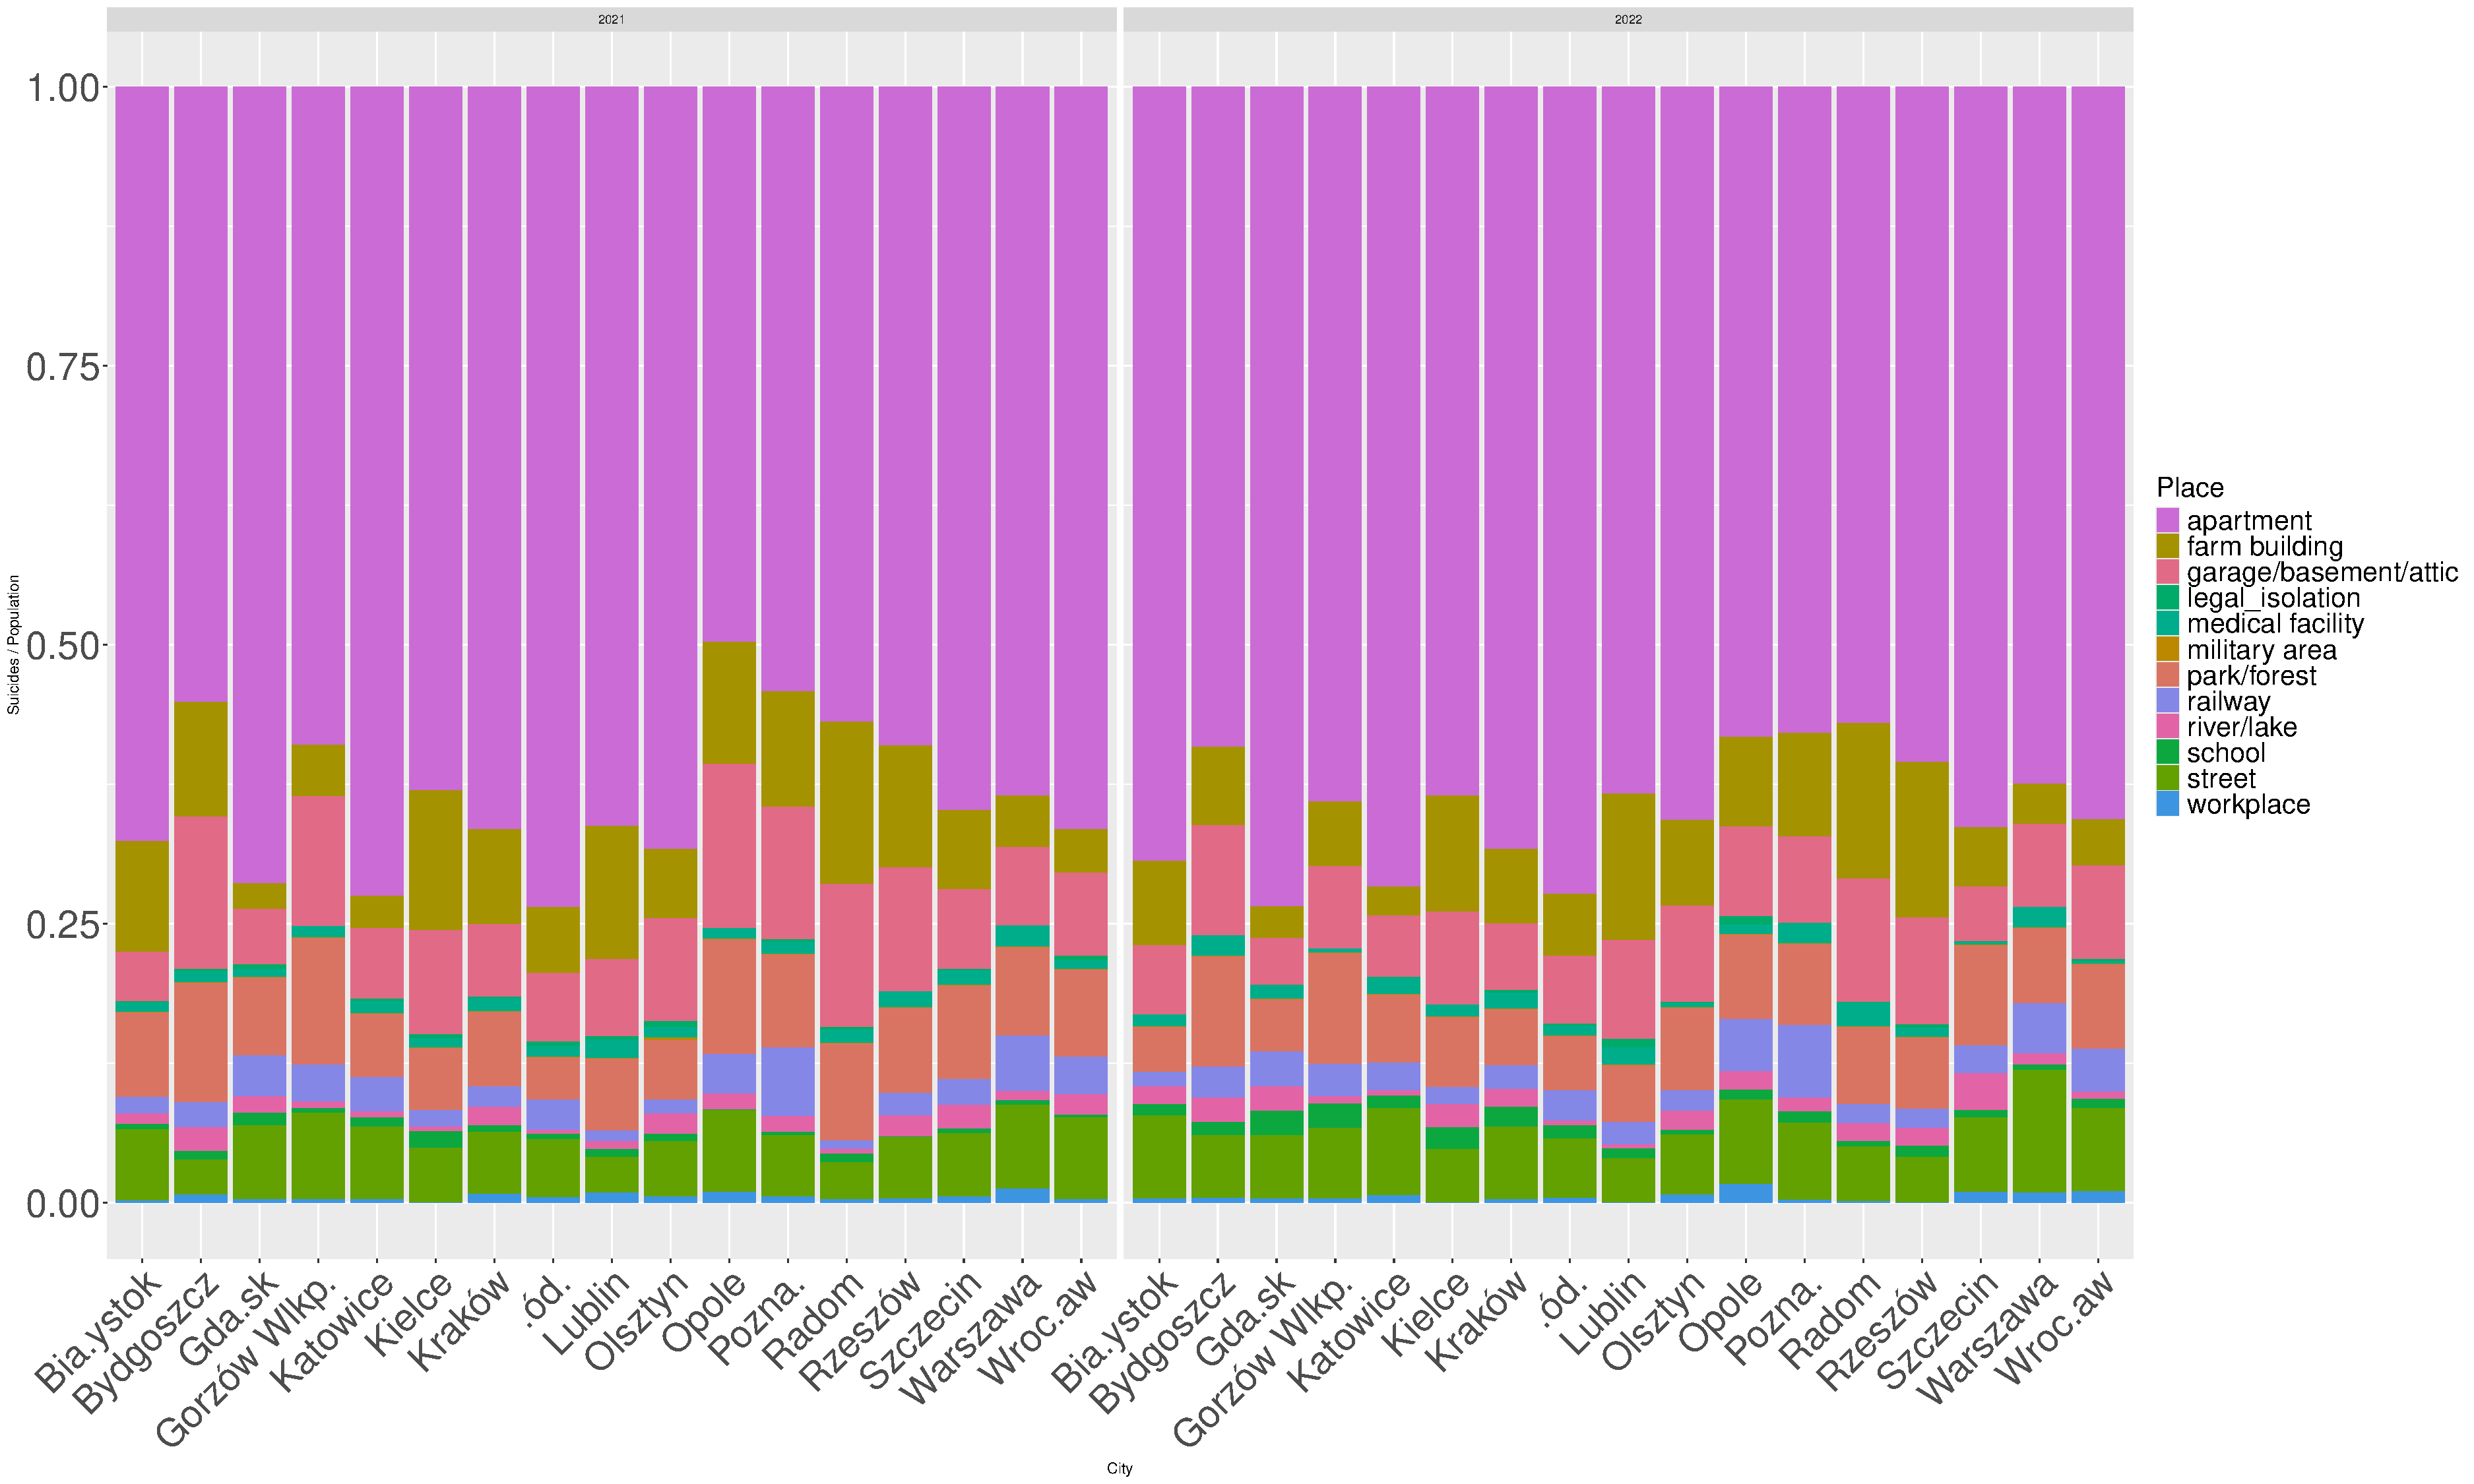
\includegraphics[width=0.65\textwidth]{imgs/place_city_att_suicides-2122.pdf}
    \caption{Attempted suicides by place in different cities in 2021 and 2022}
    \label{fig:place_city_att_suicides-2122}
\end{figure}
%
\begin{figure}[H]
    \centering
    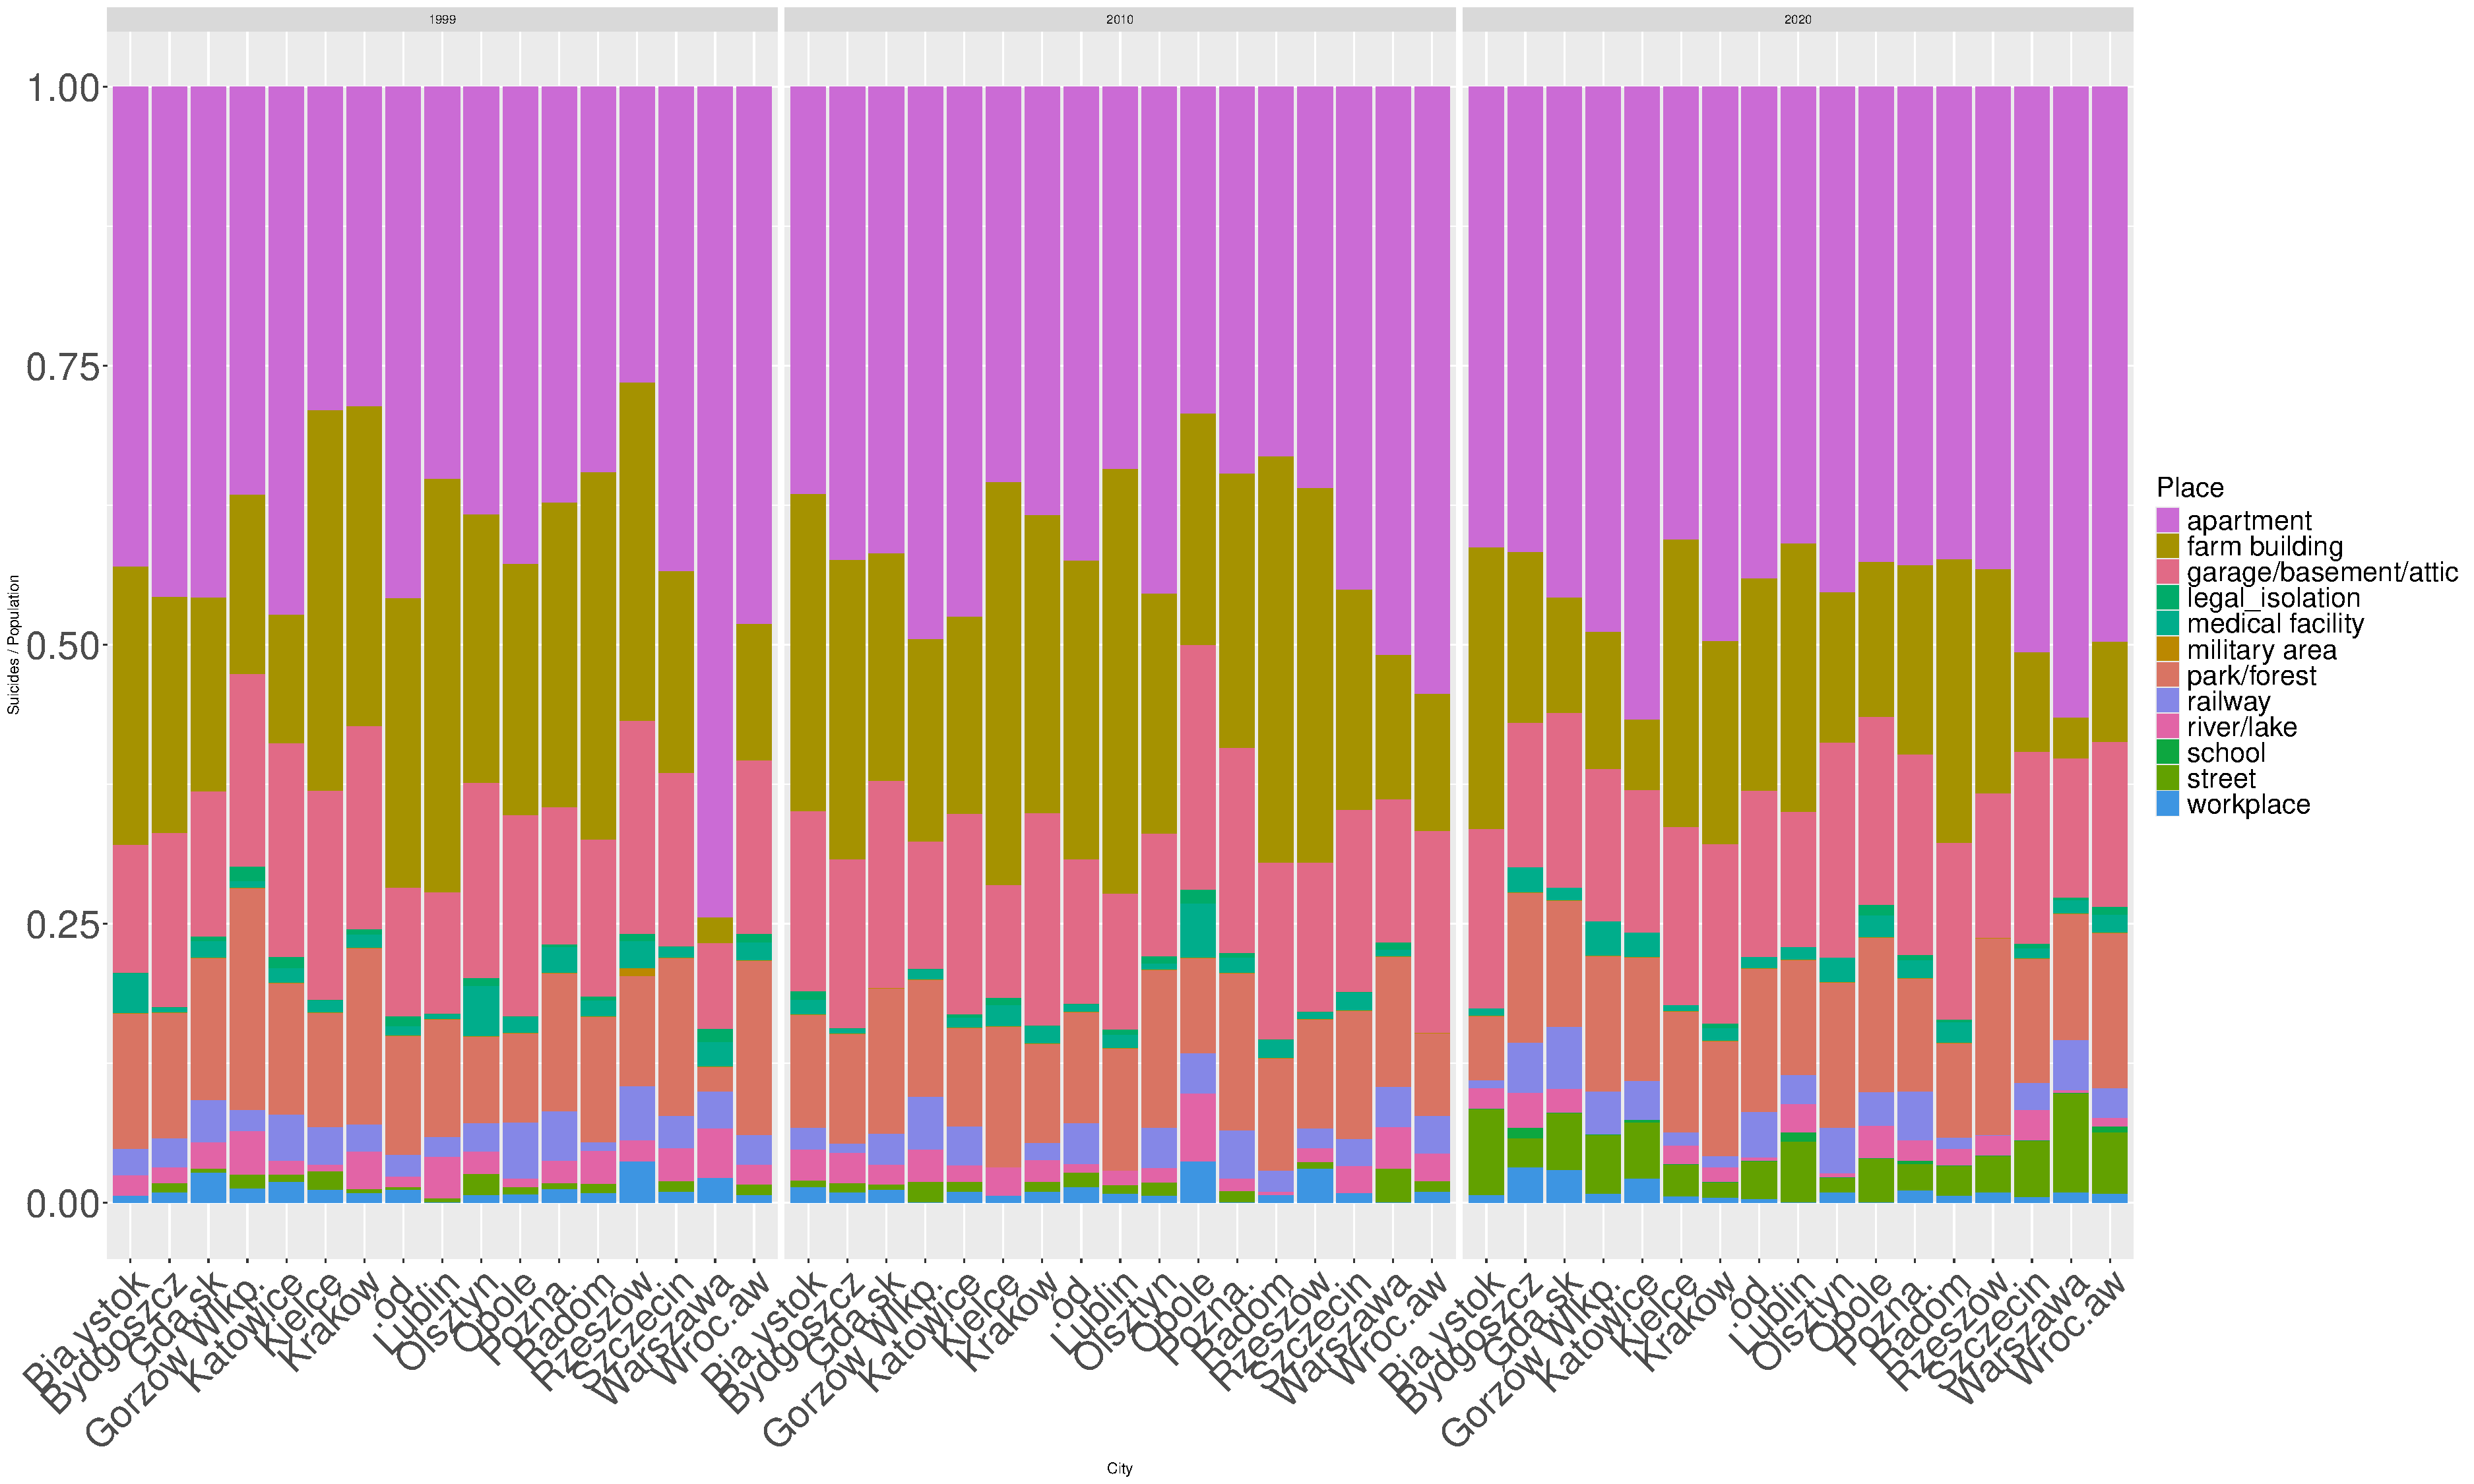
\includegraphics[width=0.65\textwidth]{imgs/place_city_fat_suicides-991020.pdf}
    \caption{Fatal suicides by place in different cities in 1999, 2010 and 2020}
    \label{fig:place_city_fat_suicides-991020}
\end{figure}

\begin{figure}[H]
    \centering
    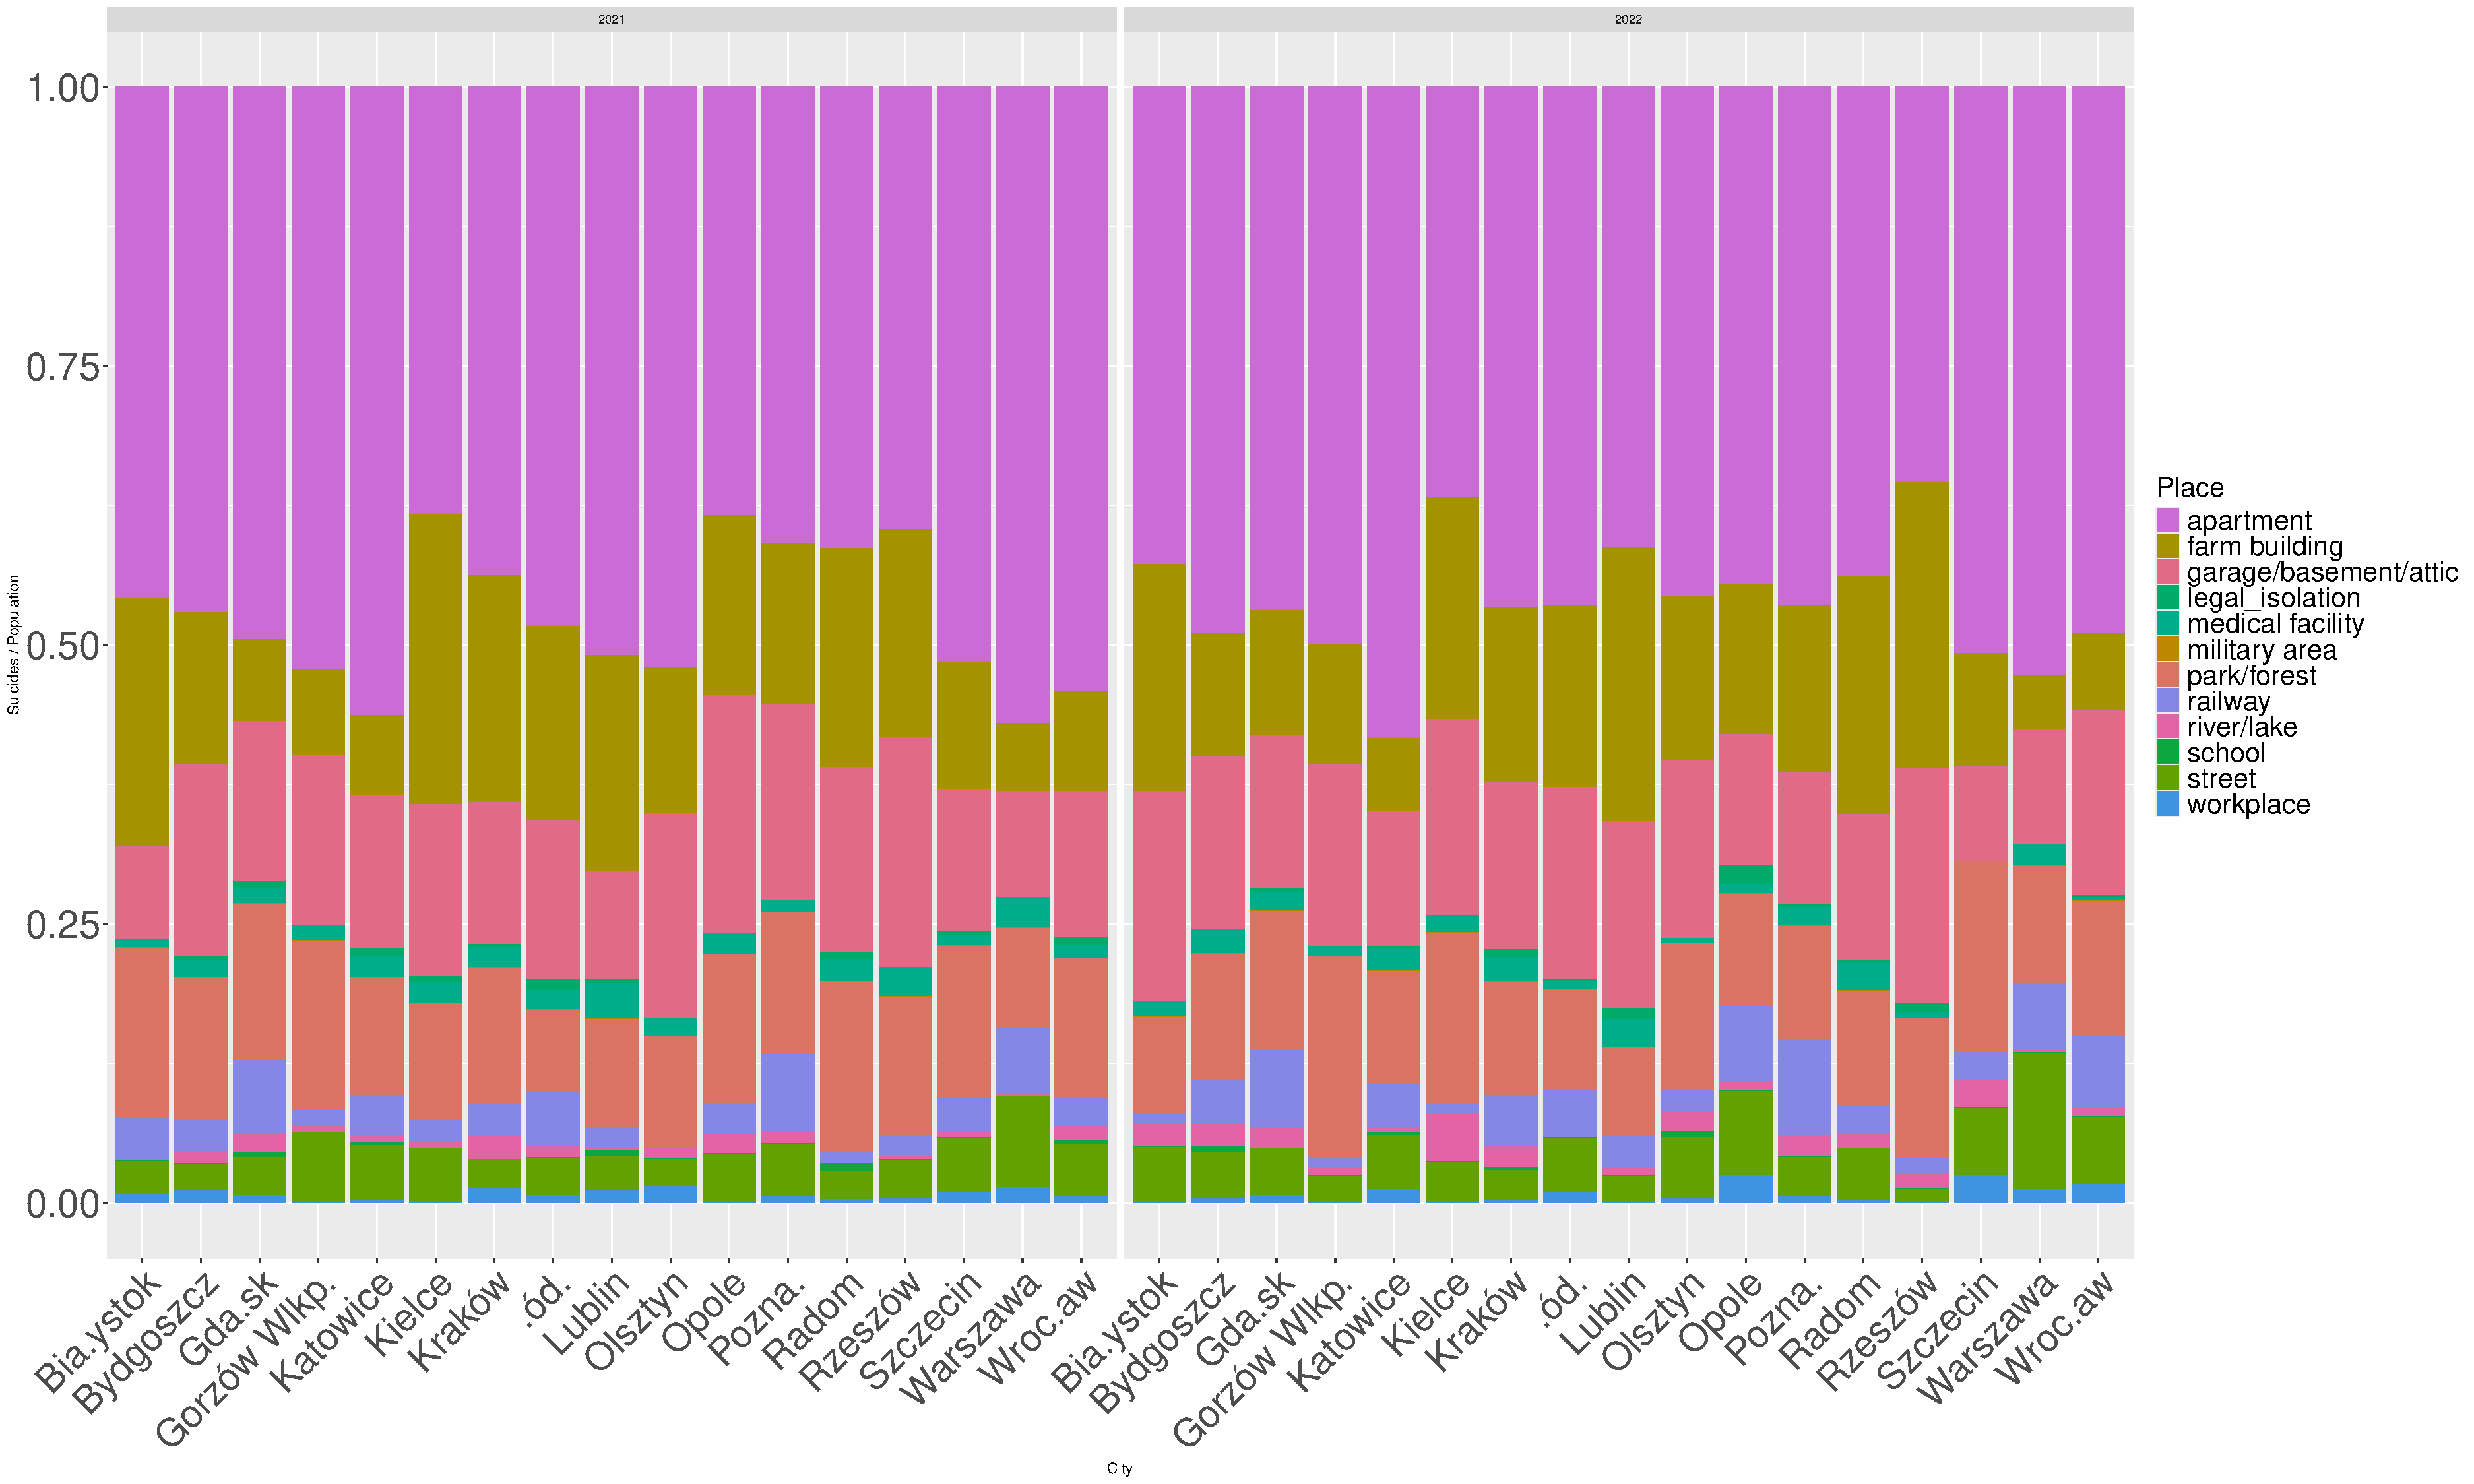
\includegraphics[width=0.65\textwidth]{imgs/place_city_fat_suicides-2122.pdf}
    \caption{Fatal suicides by place in different cities in 2021 and 2022}
    \label{fig:place_city_fat_suicides-2122}
\end{figure}
%
Figures \ref{fig:place_city_op-att-2022} and \ref{fig:place_city_op-fat-2022}
immediately draw the attention to Katowice, the city where 
the most suicide attempts (and also fatal) took place.
%
\begin{figure}[H]
    \centering
    \begin{minipage}{0.55\textwidth}
        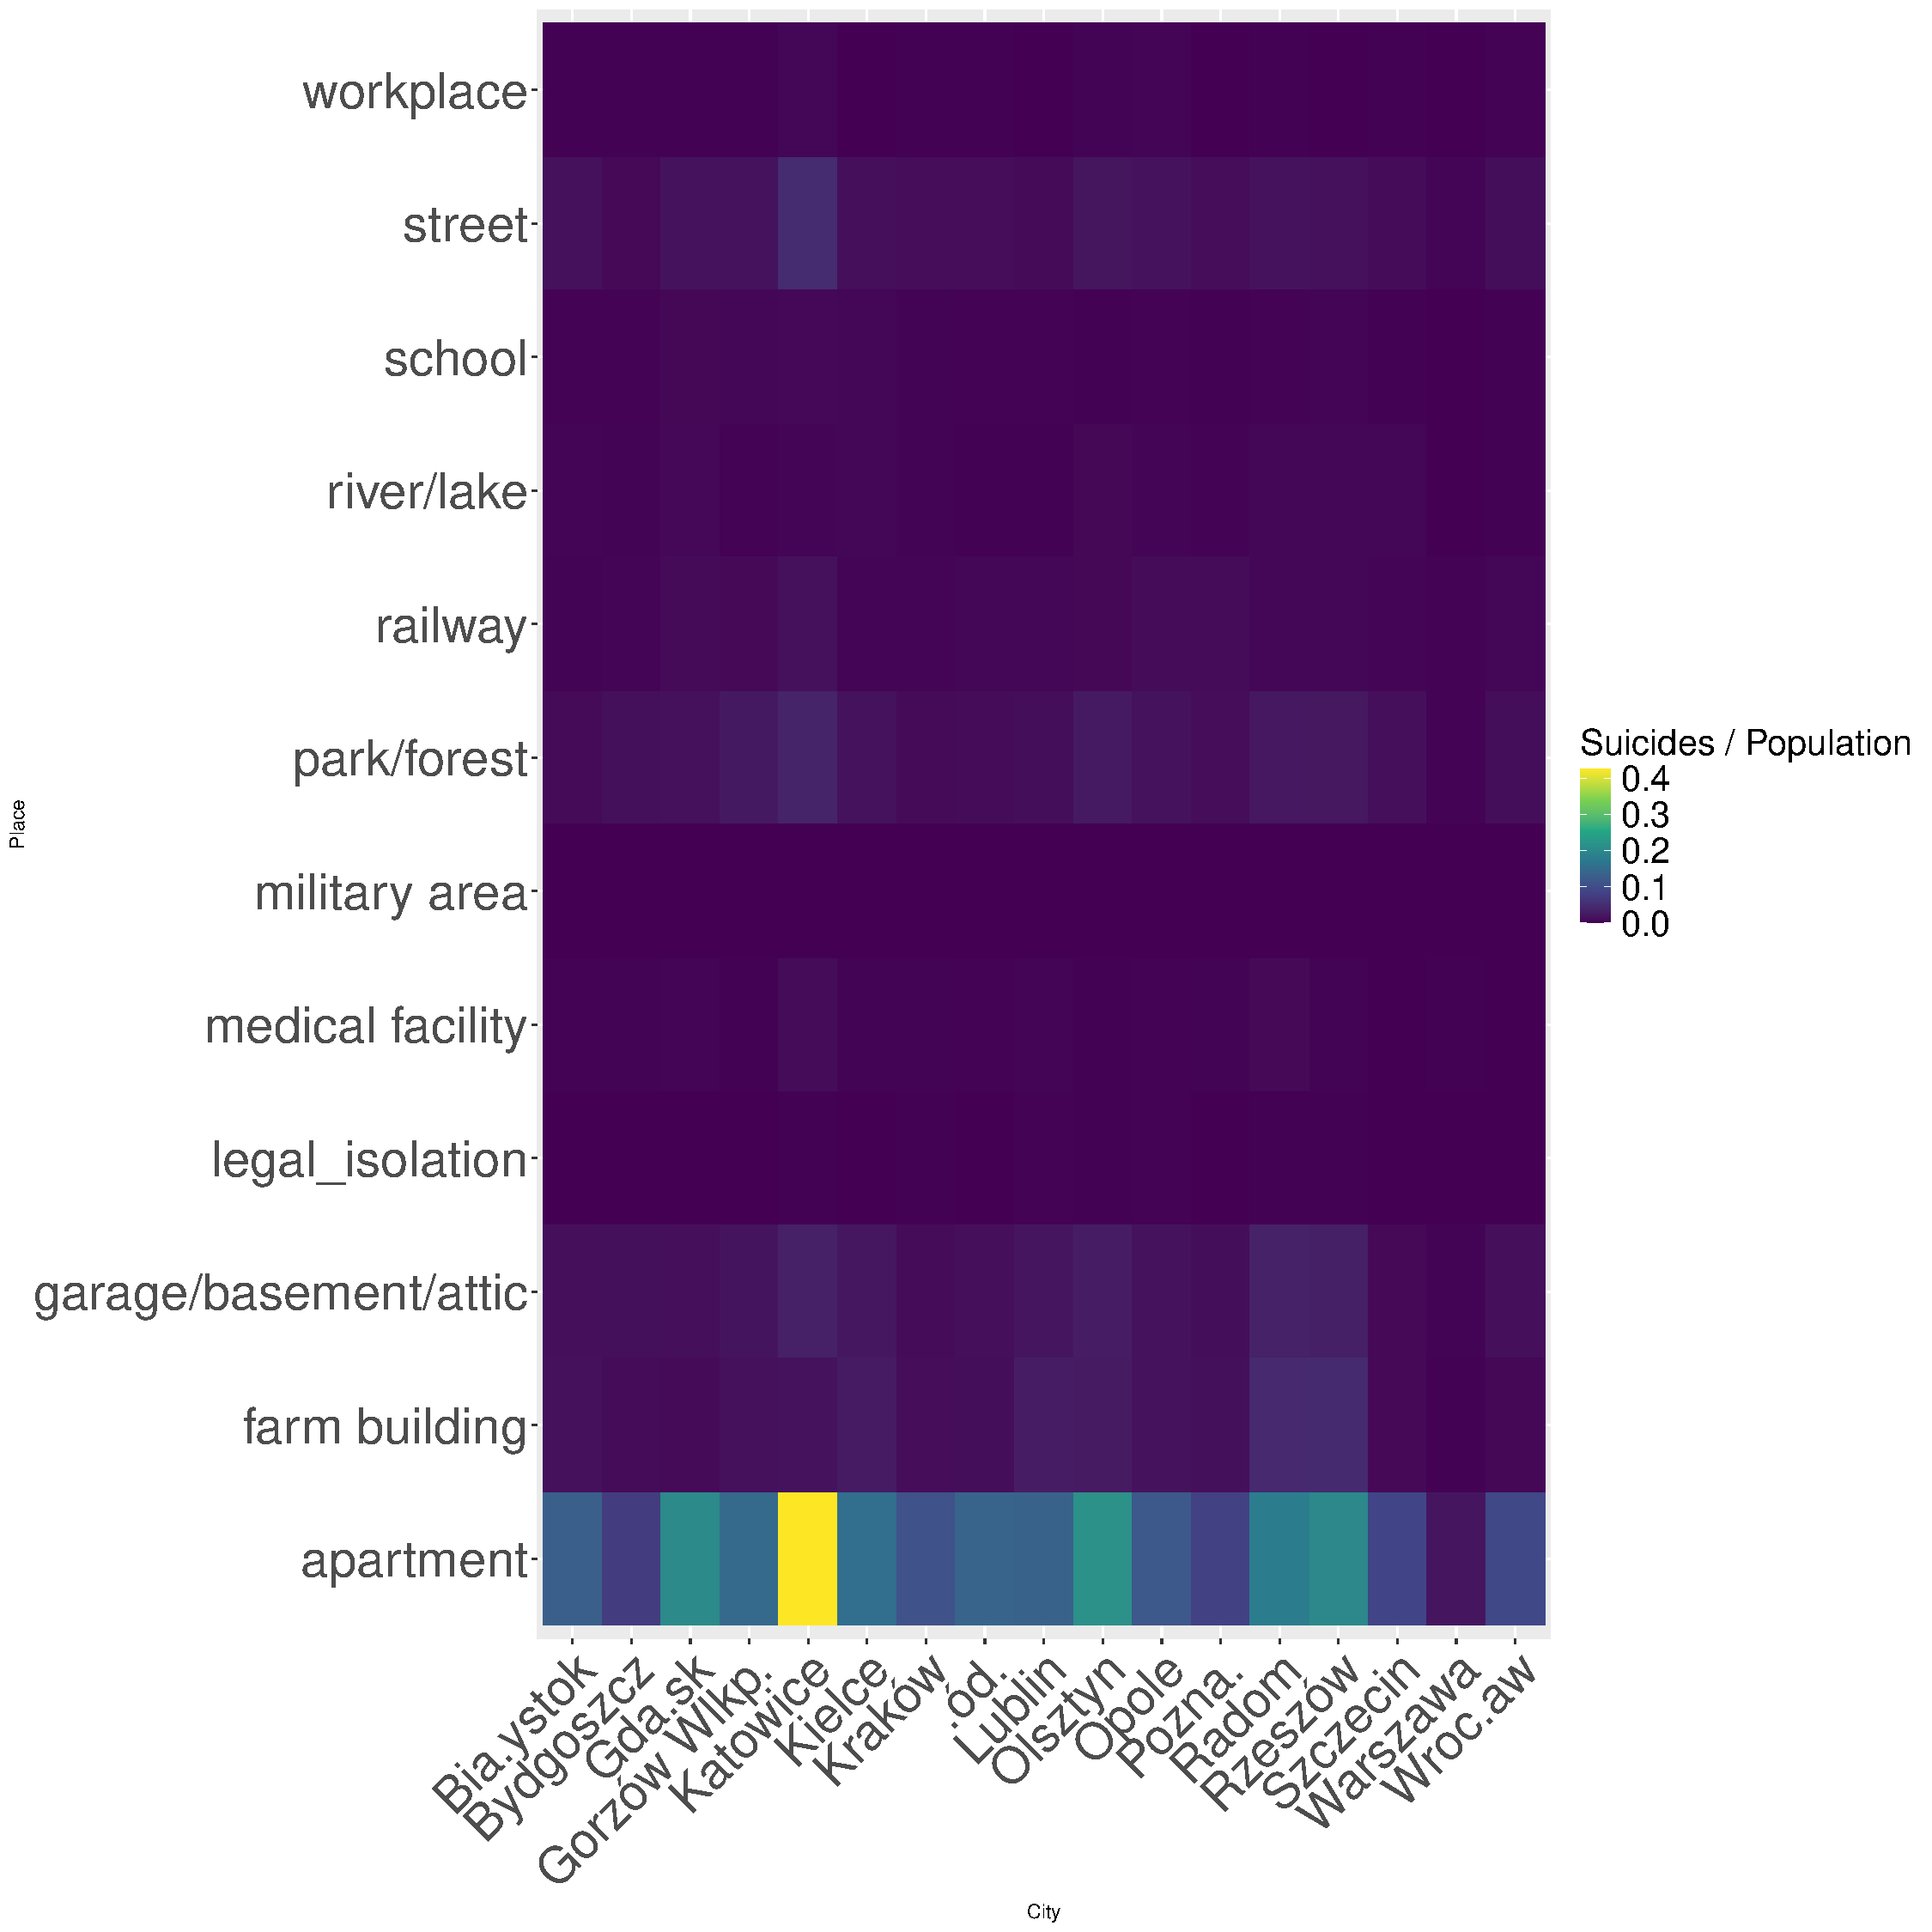
\includegraphics[width=\textwidth]{imgs/place_city_op-att-2022.pdf}
        \caption{Attempted suicides by place  in 2022 in different cities}
	\label{fig:place_city_op-att-2022}
    \end{minipage}
    \hfill
    \begin{minipage}{0.55\textwidth}
        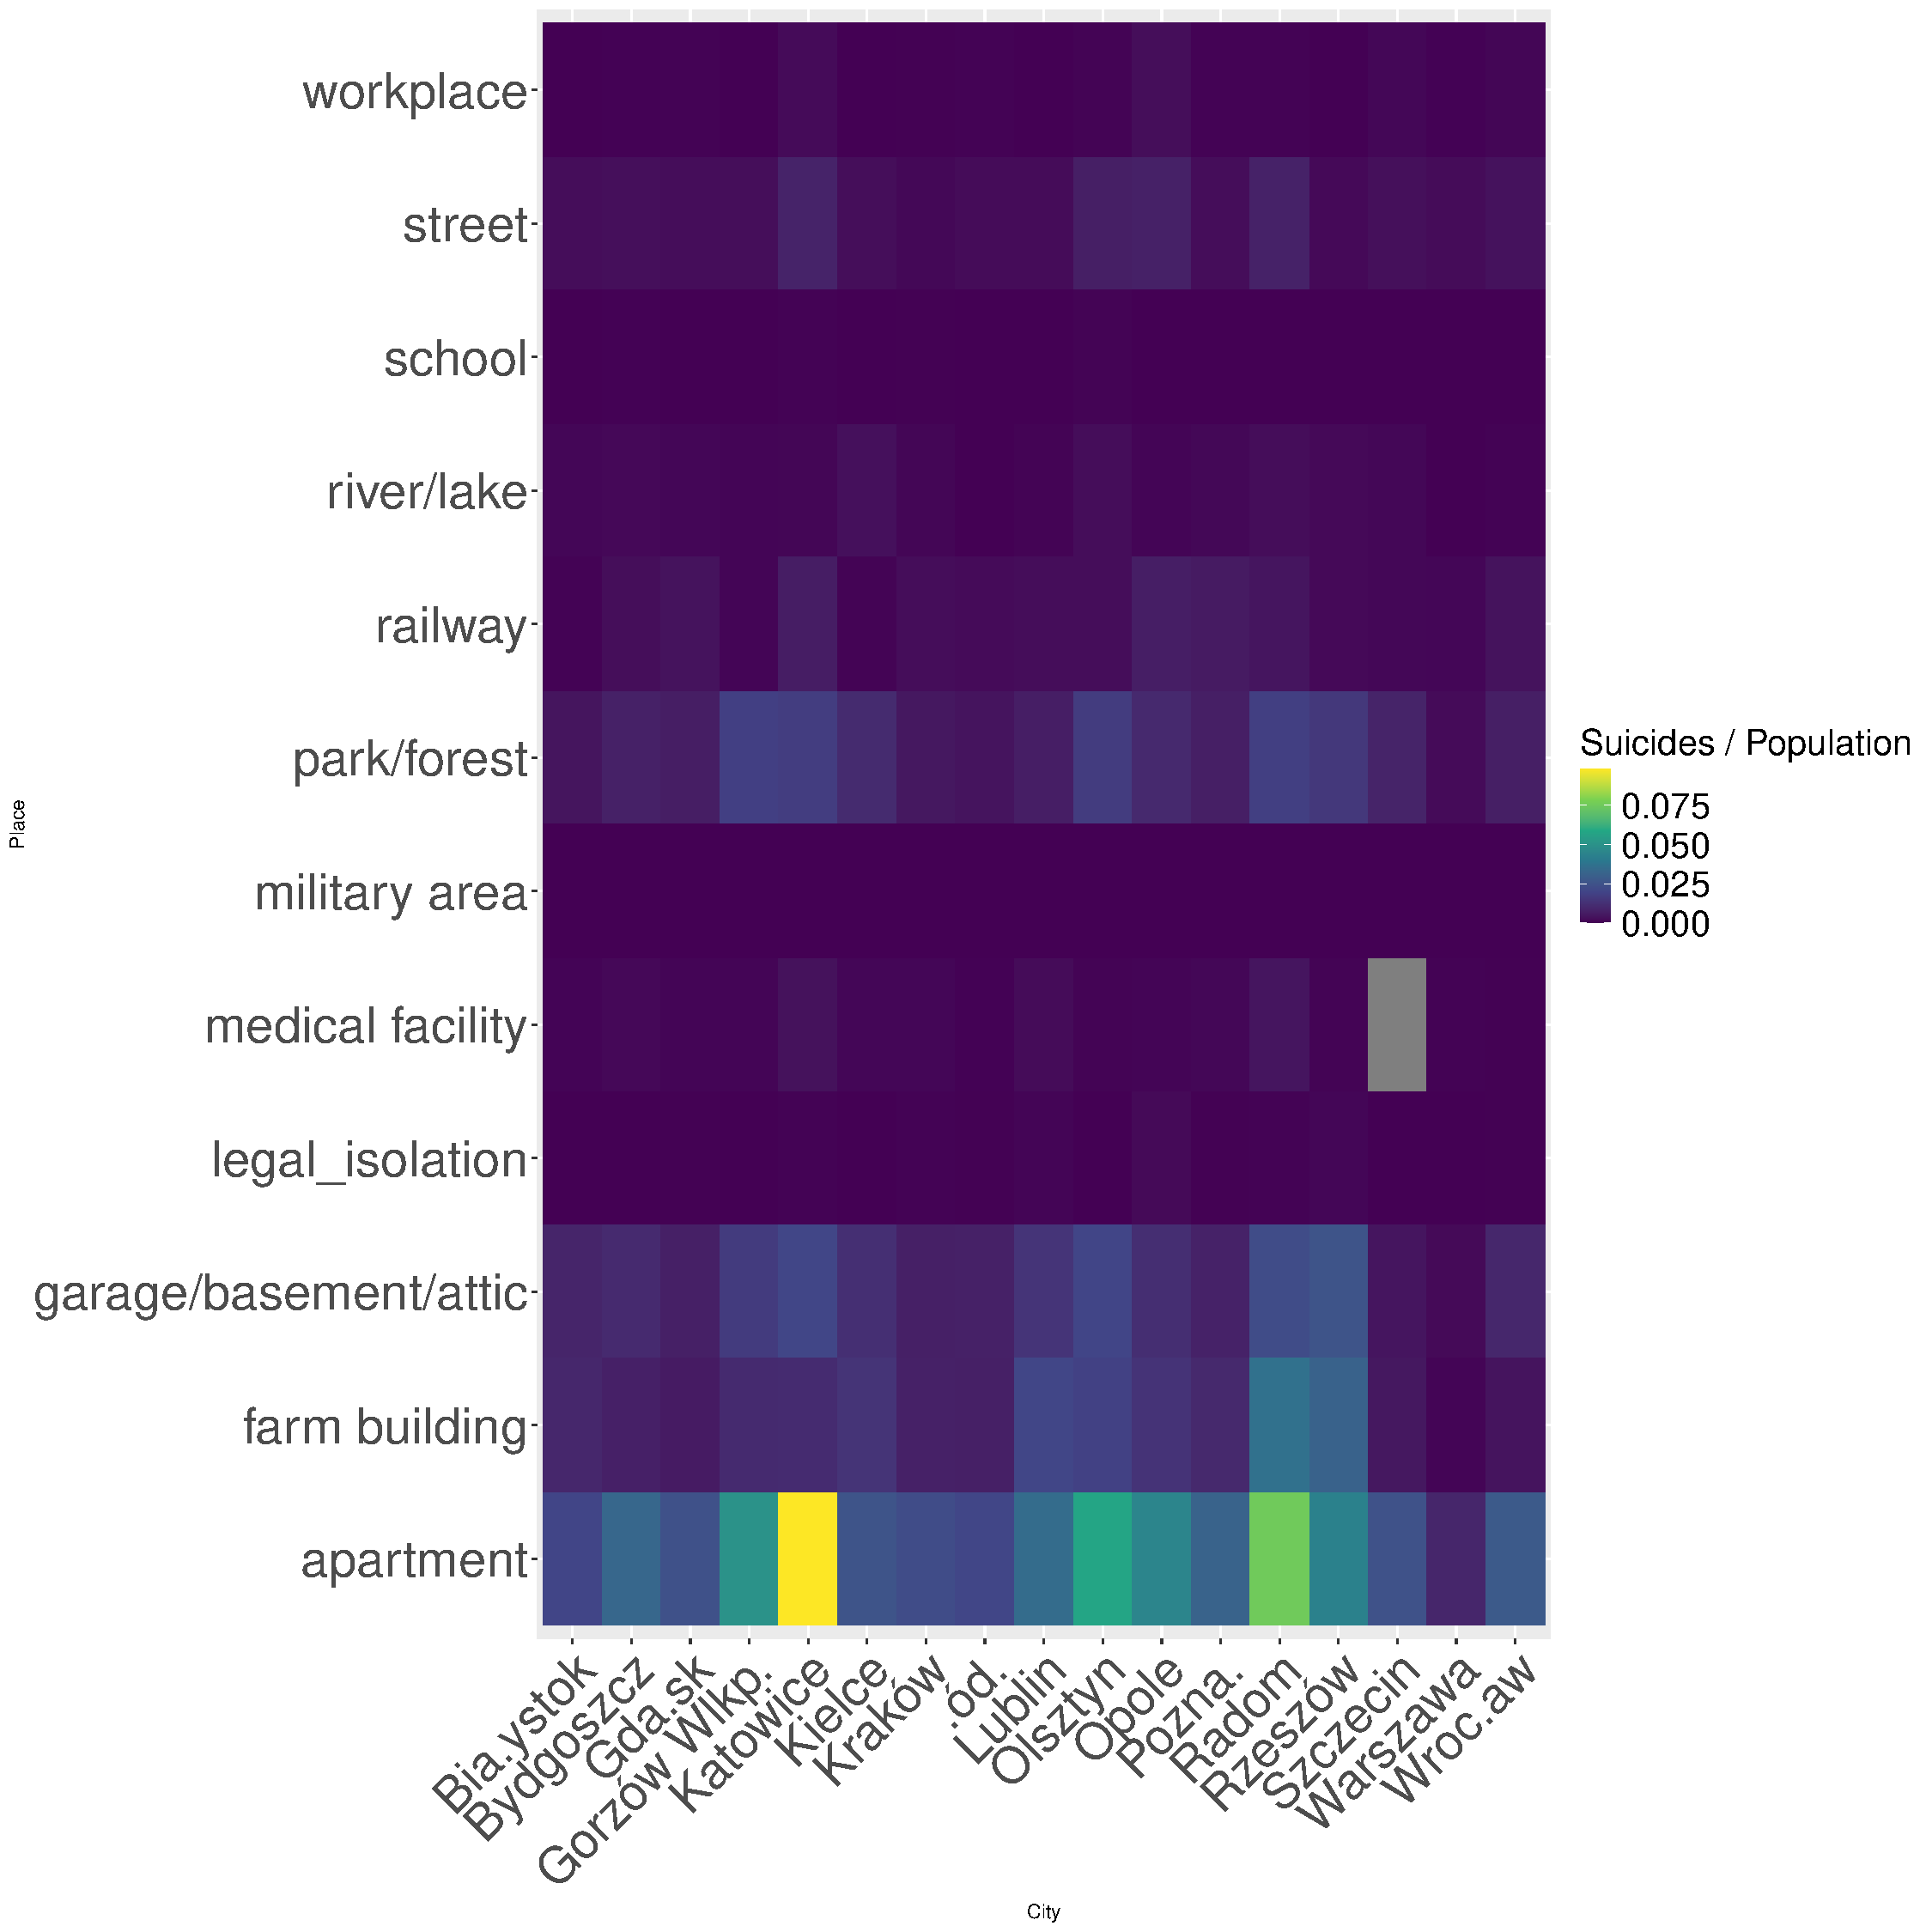
\includegraphics[width=\textwidth]{imgs/place_city_op-fat-2022.pdf}
        \caption{Fatal suicides by place  in 2022 in different cities}
	\label{fig:place_city_op-fat-2022}
    \end{minipage}
\end{figure}


\subsection{Way}
Figures \ref{way_attempted}, \ref{way_fatal}, \ref{way_foa}
show that the most common method to commit suicide in Poland is by hanging,
then follows an increasing trend in suicide attempts by taking pills,
then by self harm and by throwing from a height.
The majority of suicide attempts that resulted in a fatal outcome are 
again by hanging, then by throwing from a height (suggesting that taking pills
is not an effective method).
In Poland, what resulted as the most effective methods to commit suicide
are by shooting and by hanging, the least effective methods are by self harm
and taking pills.
Unfortunately data about attempted suicides in general are available only after 2013,
whereas data about suicides resulting in death are available since 1999. 
\begin{figure}[H]
    \centering
    \begin{minipage}{0.65\textwidth}
        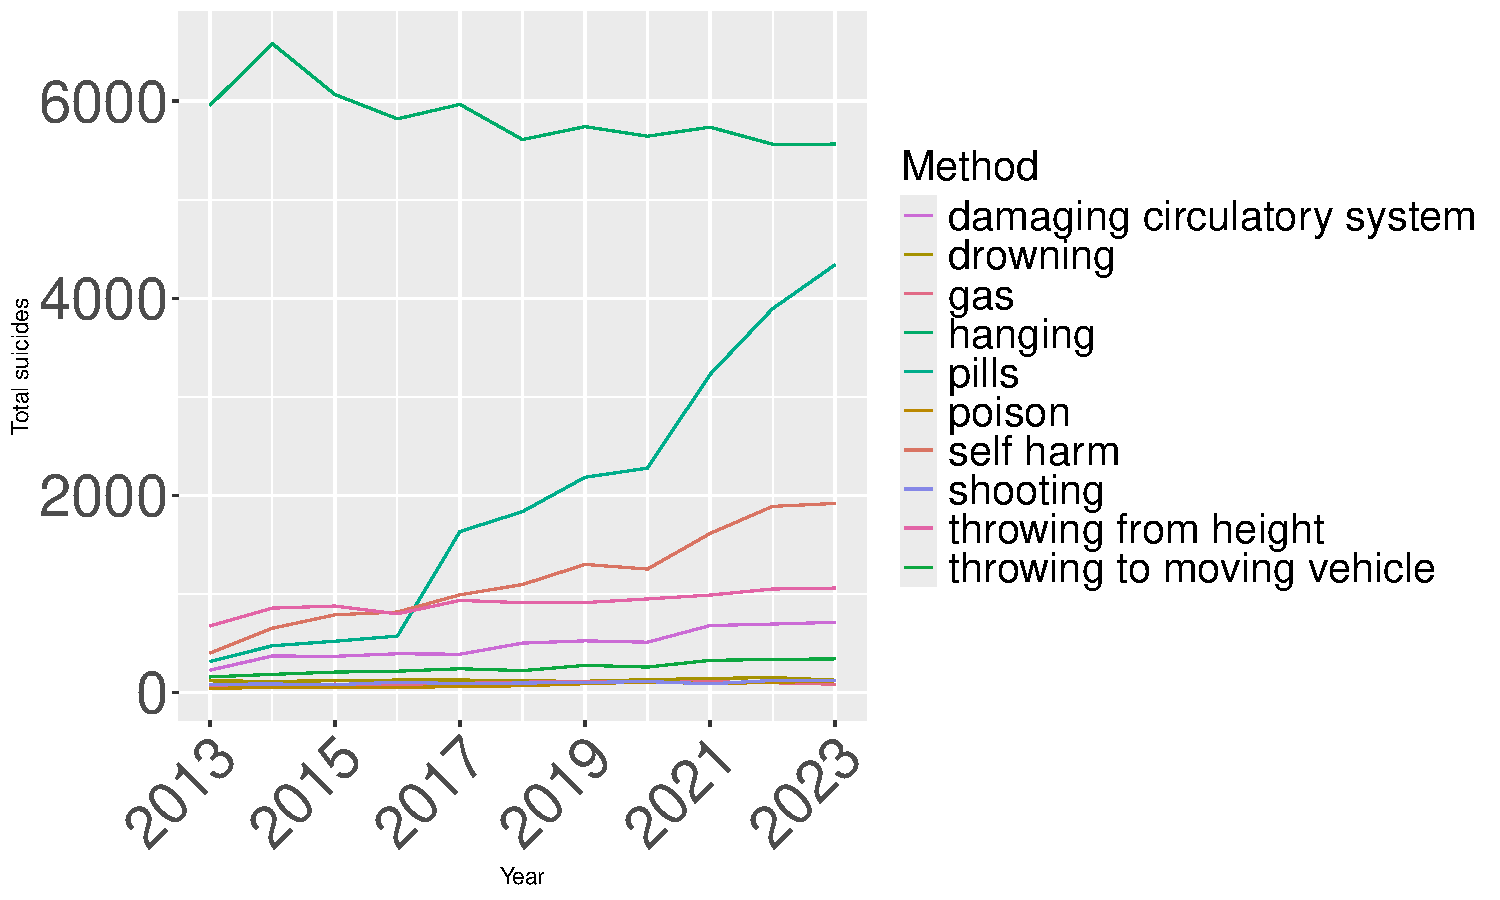
\includegraphics[width=\textwidth]{imgs/way_attempted.pdf}
        \caption{Trend of attempted suicides by way }
	\label{way_attempted}
    \end{minipage}
    \hfill
    \begin{minipage}{0.65\textwidth}
        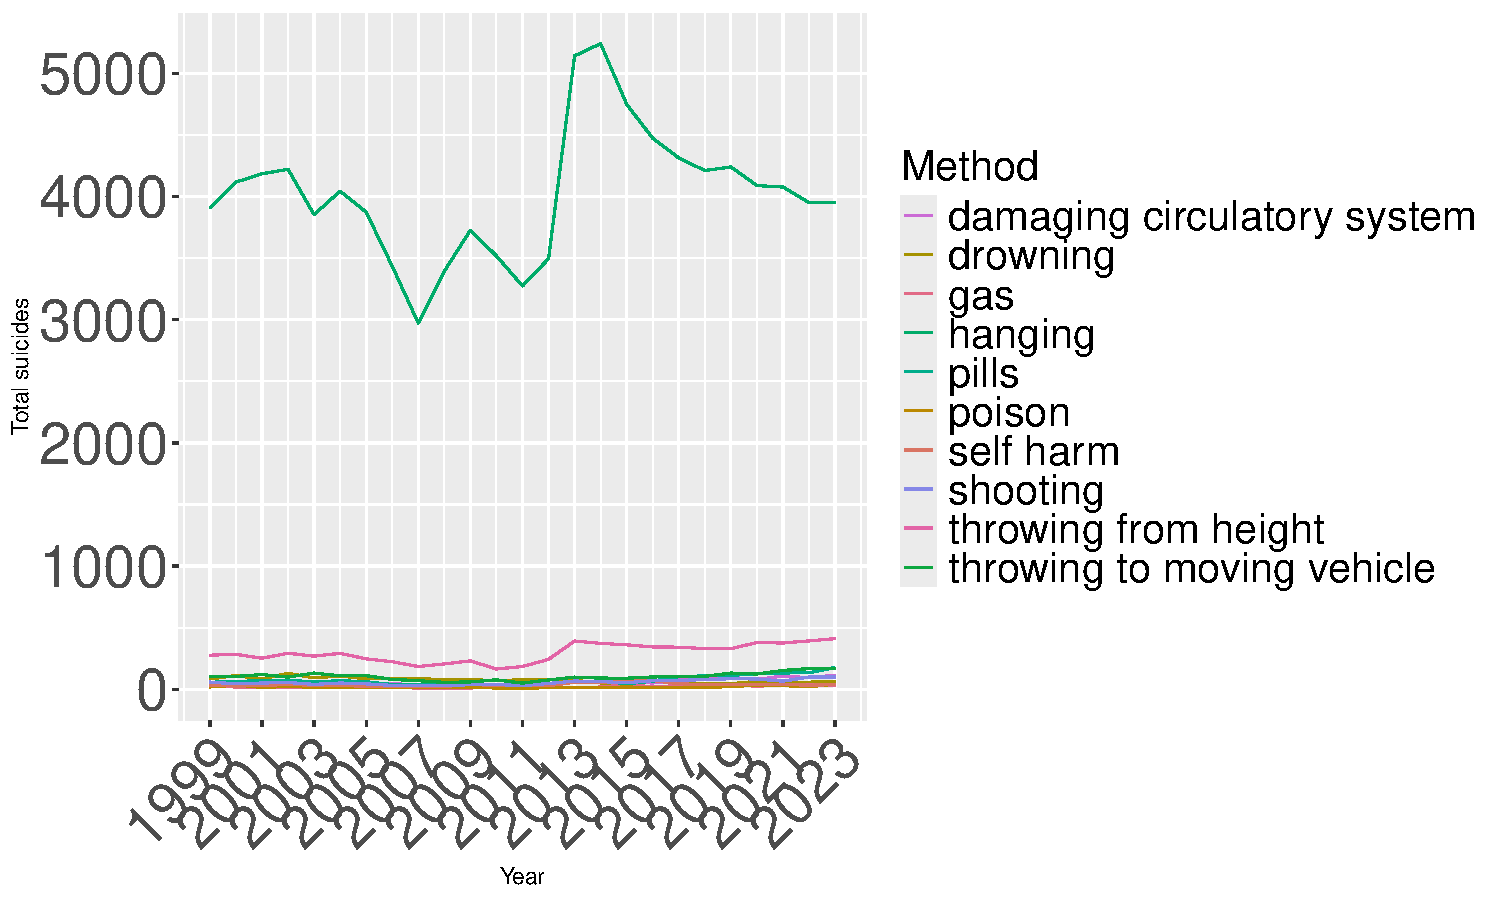
\includegraphics[width=\textwidth]{imgs/way_fatal.pdf}
        \caption{Trend of fatal suicides by way }
	\label{way_fatal}
    \end{minipage}
\end{figure}

\begin{figure}[H]
    \centering
    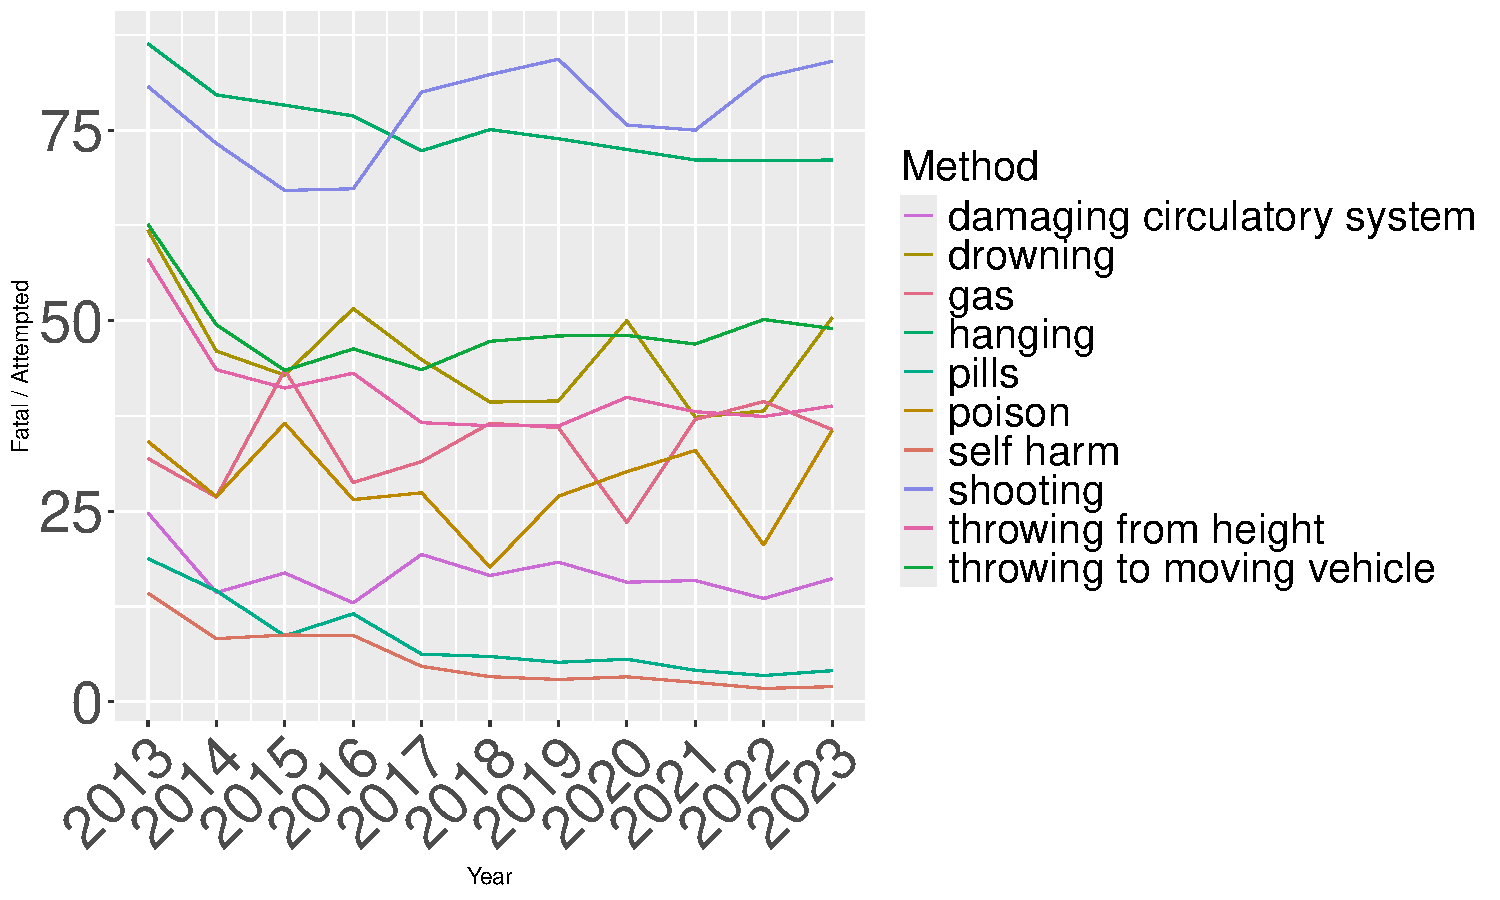
\includegraphics[width=0.65\textwidth]{imgs/way_foa.pdf}
    \caption{Trend of fatal over attempted suicides by way }
    \label{way_foa}
\end{figure}
Figure \ref{way_foa_heat}, similarly to the previous one, does not show any
evolution in the effectiveness of suicide methods.
\begin{figure}[H]
    \centering
    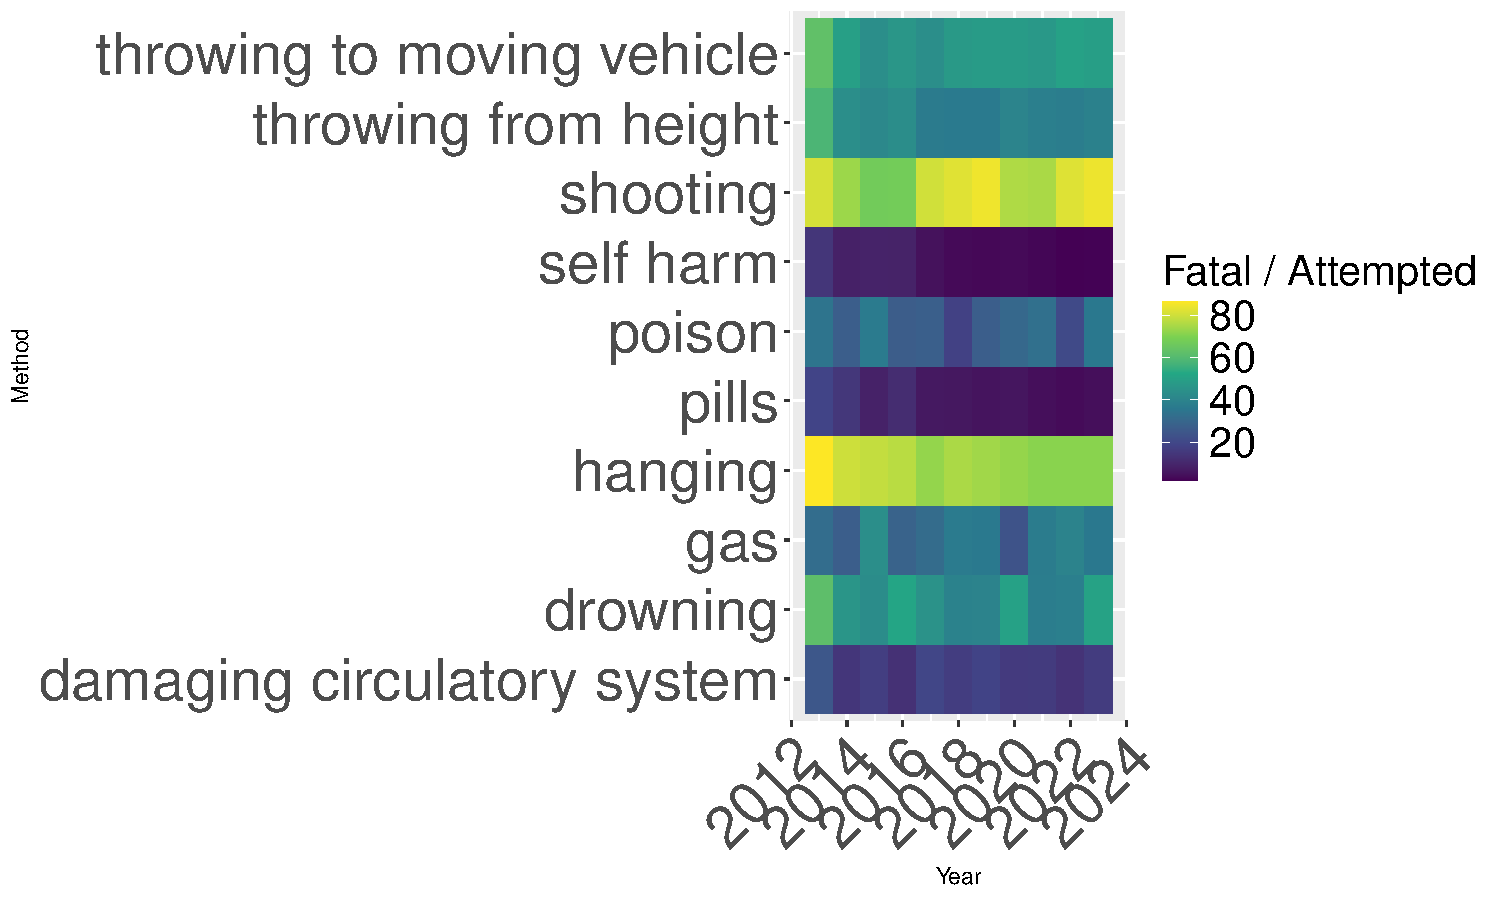
\includegraphics[width=0.65\textwidth]{imgs/way_foa_heat.pdf}
    \caption{Heatmap of fatal over attempted suicides by way }
    \label{way_foa_heat}
\end{figure}
Figures \ref{way_city_att_suicides-131722} and \ref{way_city_fat_suicides-131722}  
show that suicide attempts by taking pills increased in all cities,
in Gdańsk and Łódż in 2022 they were even more than suicide attempts by hanging,
in the section focusing on sex it was shown that a great number of females 
attempted suicide in Gdańsk, this might suggest that taking pills is a popular
method among females, a similar reasoning can be applied to suicide attempts by self harm,
however, such speculations cannot be proved, these correlations could be caused 
by a hidden variable that would not be easy to uncover.
An argument against this hypothesis could simply be that suicide attempts by taking 
pills increased in percentage in all the cities and not just Gdańsk or Łodż.
\begin{figure}[H]
    \centering
    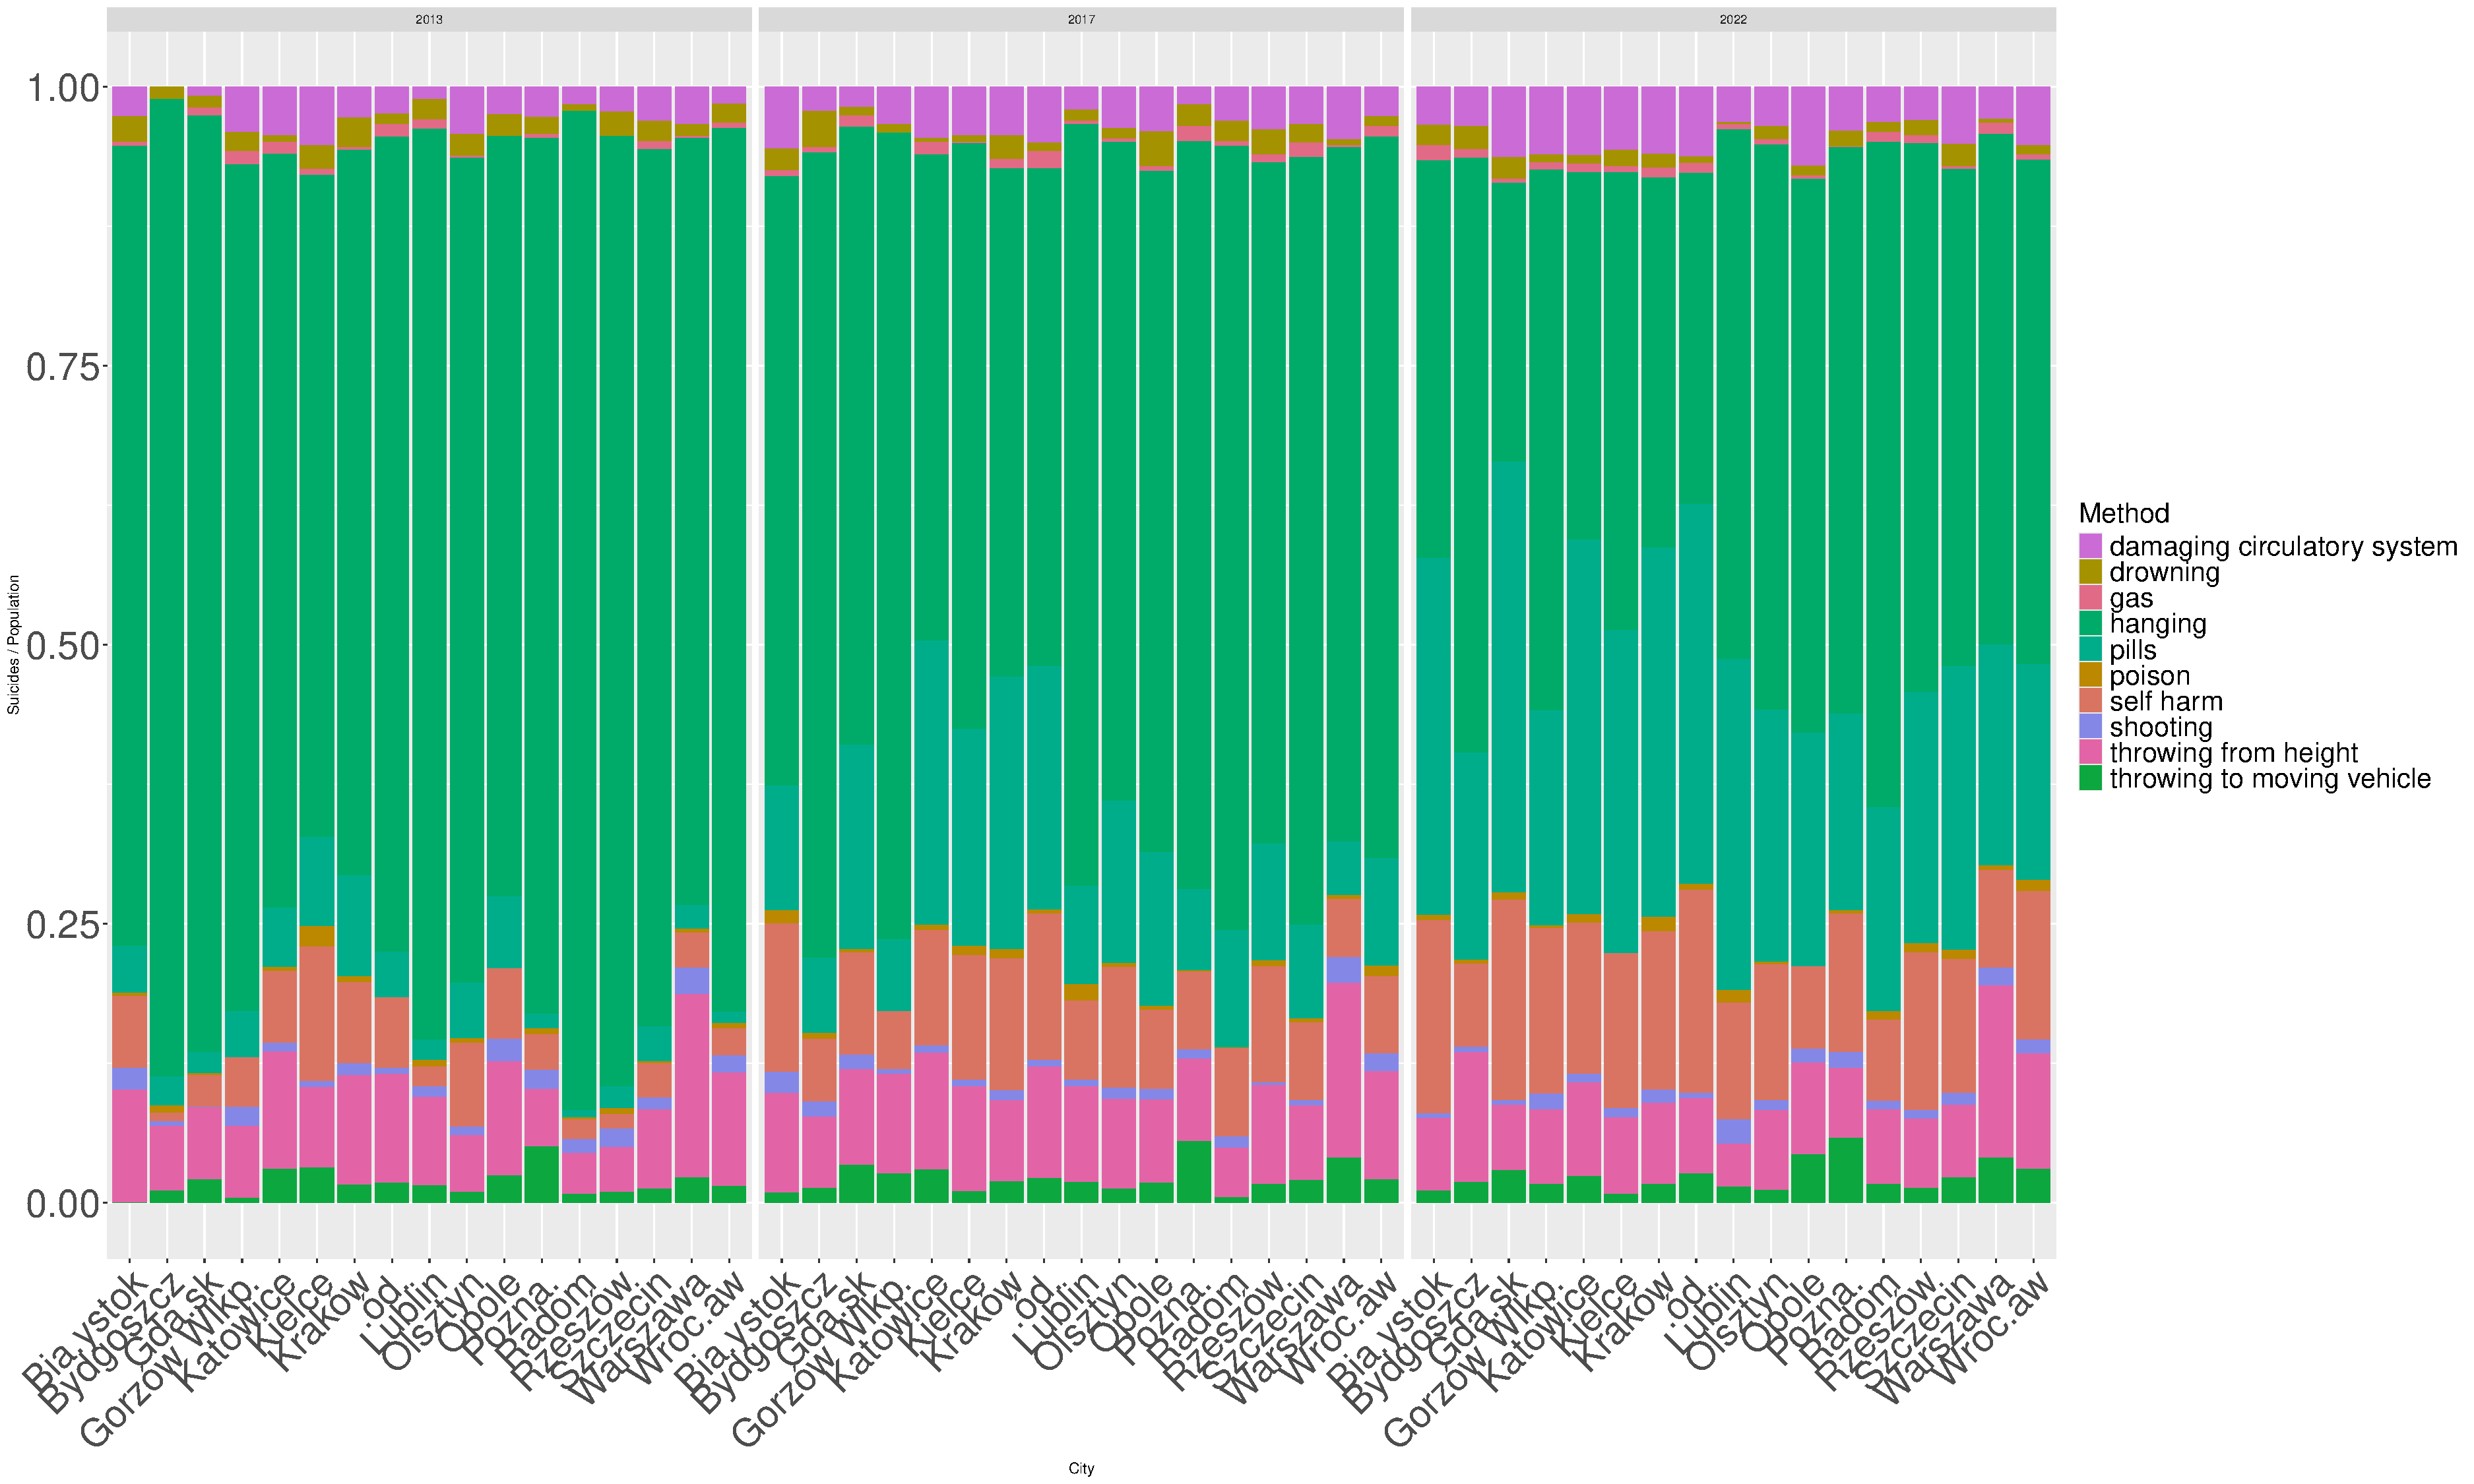
\includegraphics[width=0.65\textwidth]{imgs/way_city_att_suicides-131722.pdf}
    \caption{Attempted suicides by way  in 2013, 2017 and 2022}
    \label{way_city_att_suicides-131722}
\end{figure}

\begin{figure}[H]
    \centering
    \includegraphics[width=0.65\textwidth]{imgs/way_city_fat_suicides-131722.pdf}
    \caption{Fatal suicides by way  in 2013, 2017 and 2022}
    \label{way_city_fat_suicides-131722}
\end{figure}
Figures \ref{way_city_op-att-2022} and \ref{way_city_op-fat-2022}
remark how hanging is the most frequently adopted method to commit suicide resulting
in death and that Radom was the city with the greatest number of cases by population: 156 every 100000.
The other most affected cities were Katowice, Rzeszow and Olsztyn.
\begin{figure}[H]
    \centering
    \begin{minipage}{0.65\textwidth}
        \includegraphics[width=\textwidth]{imgs/way_city_op-att-2022.pdf}
        \caption{Attempted suicides by way  in 2022 in different cities}
	\label{way_city_op-att-2022}
    \end{minipage}
    \hfill
    \begin{minipage}{0.65\textwidth}
        \includegraphics[width=\textwidth]{imgs/way_city_op-fat-2022.pdf}
        \caption{Fatal suicides by way  in 2022 in different cities}
	\label{way_city_op-fat-2022}
    \end{minipage}
\end{figure}
%
%
%
%
\subsection{Reason}
%
%
Figures \ref{reason_attempted}, \ref{reason_fatal}, \ref{reason_foa}
show that the most common reason for attempting suicide 
is mental illness, followed by heartbreak and family problems.
When considering fatal suicide attempts, mental illness is the reason 
that increased the most, although this might be regarded as a reason lead to
by other reasons; this is why it is not easy to decide what are the social
diseases to work on to contain the phenomenon of suicides as much as possible. 
Suicide attempts because of school/work problems are unfortunately increasing: in 2020, 2021, 2022 and 2023
they were respectively 159, 240, 313 and 322.
The reason that caused the highest fatality ratio is physical illness, followed by disability,
loss of health and committing a crime, interestingly enough, none of the most common reasons for attempting
suicide is among the ones with highest fatality ratio.
Unfortunately, only data about fatal suicide attempts are available since 1999,
whereas data about all attempts are available only since 2013.
\begin{figure}[H]
    \centering
    \begin{minipage}{0.65\textwidth}
        \includegraphics[width=\textwidth]{imgs/reason_attempted.pdf}
        \caption{Trend of attempted suicides by reason }
	\label{reason_attempted}
    \end{minipage}
    \hfill
    \begin{minipage}{0.65\textwidth}
        \includegraphics[width=\textwidth]{imgs/reason_fatal.pdf}
        \caption{Trend of fatal suicides by reason }
	\label{reason_fatal}
    \end{minipage}
\end{figure}

\begin{figure}[H]
    \centering
    \includegraphics[width=0.65\textwidth]{imgs/reason_foa.pdf}
    \caption{Trend of fatal over attempted suicides by reason }
    \label{reason_foa}
\end{figure}

\begin{figure}[H]
    \centering
    \includegraphics[width=0.65\textwidth]{imgs/reason_foa_heat.pdf}
    \caption{Heatmap of fatal over attempted suicides by reason }
\end{figure}
%
%
In figures \ref{fig:reason_city_att_suicides-131722} and \ref{fig:reason_city_fat_suicides-131722}
it is shown that family problems, physical illness and poor economical conditions 
decreased as the percentage of all reasons that lead to suicide (both attempted and fatal suicides),
mental illness and school/work problems on the other hand increased.
\begin{figure}[H]
    \centering
    \includegraphics[width=0.65\textwidth]{imgs/reason_city_att_suicides-131722.pdf}
    \caption{Attempted suicides by reason  in 2013, 2017 and 2022}
    \label{fig:reason_city_att_suicides-131722}
\end{figure}

\begin{figure}[H]
    \centering
    \includegraphics[width=0.65\textwidth]{imgs/reason_city_fat_suicides-131722.pdf}
    \caption{Fatal suicides by reason  in 2013, 2017 and 2022}
    \label{fig:reason_city_fat_suicides-131722}
\end{figure}
In figures \ref{fig:reason_city_op-att-2022} and \ref{fig:reason_city_op-fat-2022}
it is again confirmed that mental illness is the most common reason for attempting
suicide and that Katowice, Rzeszow and Radom are the most problematic.
\begin{figure}[H]
    \centering
    \begin{minipage}{0.65\textwidth}
        \includegraphics[width=\textwidth]{imgs/reason_city_op-att-2022.pdf}
        \caption{Attempted suicides by reason  in 2022 in different cities}
	\label{fig:reason_city_op-att-2022}
    \end{minipage}
    \hfill
    \begin{minipage}{0.65\textwidth}
        \includegraphics[width=\textwidth]{imgs/reason_city_op-fat-2022.pdf}
        \caption{Fatal suicides by reason  in 2022 in different cities}
	\label{fig:reason_city_op-fat-2022}
    \end{minipage}
\end{figure}


\subsection{Status}
As shown in figures \ref{fig:status_attempted} and \ref{fig:status_fatal},
the majority of people attempting suicide were single, then married.
Regarding suicides with a fatal outcome, since 2014, the numbers have been decreasing
for married
people and have been increasing for single people.
\begin{figure}[H]
    \centering
    \begin{minipage}{0.65\textwidth}
        \includegraphics[width=\textwidth]{imgs/status_attempted.pdf}
        \caption{Trend of attempted suicides by civil status }
	\label{fig:status_attempted}
    \end{minipage}
    \hfill
    \begin{minipage}{0.65\textwidth}
        \includegraphics[width=\textwidth]{imgs/status_fatal.pdf}
        \caption{Trend of fatal suicides by civil status }
	\label{fig:status_fatal}
    \end{minipage}
\end{figure}
For all of the social statuses the fatality of 
the attempts seems to have been decreasing: again,
this is not because people have been failing more and more often when attempting suicide, 
but rather because many more cases have been registered as attempted during the last years
than they have been during the first years the data have been made available since,
and this could be justified by the technical reason epxlained at the beginning of the document.
\begin{figure}[H]
    \centering
    \includegraphics[width=0.65\textwidth]{imgs/status_foa.pdf}
    \caption{Trend of fatal over attempted suicides by civil status }
	\label{fig:status_foa}
\end{figure}

\begin{figure}[H]
    \centering
    \includegraphics[width=0.65\textwidth]{imgs/status_foa_heat.pdf}
    \caption{Heatmap of fatal over attempted suicides by civil status }
    \label{fig:status_foa_heat}
\end{figure}
By what is shown in figure \ref{fig:status_city_att_suicides-2122}
the first thing that can be noticed is the peak in the percentage of
single people attempting suicide in Gdańsk in 2021, 2022 and 2023,
with a similar reasoning to the one made regarding suicide attempts
by taking pills in Gdańsk, it could be investigated whether single
women are more likely to commit suicide; if that was the case then 
it could make sense to investigate whether heartbreak was a major reason
for attempting suicide in the last years but Gdańsk does not display any relevant
peak in \ref{fig:reason_city_att_suicides-131722}, this could either mean that 
single women are more likely to commit suicide but not because of 
a heartbreak or that the correlation is simply coincidential or caused
by a hidden variable.
\begin{figure}[H]
    \centering
    \includegraphics[width=0.65\textwidth]{imgs/status_city_att_suicides-991020.pdf}
    \caption{Attempted suicides by civil status  in 1999, 2010 and 2020}
    \label{fig:status_city_att_suicides-991020}
\end{figure}

\begin{figure}[H]
    \centering
    \includegraphics[width=0.65\textwidth]{imgs/status_city_att_suicides-2122.pdf}
    \caption{Attempted suicides by civil status  in 2021 and 2022}
    \label{fig:status_city_att_suicides-2122}
\end{figure}

\begin{figure}[H]
    \centering
    \includegraphics[width=0.65\textwidth]{imgs/status_city_fat_suicides-991020.pdf}
    \caption{Fatal suicides by civil status  in 1999, 2010 and 2020}
    \label{fig:status_city_fat_suicides-991020}
\end{figure}

\begin{figure}[H]
    \centering
    \includegraphics[width=0.65\textwidth]{imgs/status_city_fat_suicides-2122.pdf}
    \caption{Fatal suicides by civil status  in 2021 and 2022}
    \label{fig:status_city_fat_suicides-2122}
\end{figure}
%
%
Figures \ref{fig:status_city_op-att-2022} and \ref{fig:status_city_op-fat-2022}
confirm that the majority of the cases of suicide attempts are committed
by single and married people in Katowice, Radom and Rzeszów.
\begin{figure}[H]
    \centering
    \begin{minipage}{0.55\textwidth}
        \includegraphics[width=\textwidth]{imgs/status_city_op-att-2022.pdf}
        \caption{Attempted suicides by civil status  in 2022 in different cities}
	\label{fig:status_city_op-att-2022}
    \end{minipage}
    \hfill
    \begin{minipage}{0.55\textwidth}
        \includegraphics[width=\textwidth]{imgs/status_city_op-fat-2022.pdf}
        \caption{Fatal suicides by civil status  in 2022 in different cities}
        \label{fig:status_city_op-fat-2022}
    \end{minipage}
\end{figure}


\subsection{Education}
The plots \ref{fig:education_attempted}, \ref{fig:education_fatal} and
\ref{fig:education_foa}
show an unprecedent behaviour: the attempted suicides by
people with a basic, medium or technical/professional education decreased until 2011 and then
increased. The trend in the suicide attempts with a fatal outcome decreased
until 2011 for the previous categories (which are also the three with the greatest numbers)
but did not increase after.
The reason for the dissimilarity between the trends focusing on education and the more general
ones such as those focusing on sex (\ref{fig:sex_attempted})
or on total values (\ref{fig:poland_general})
is that the cases labeled with an education level are the minority,
as an example, in 2022 there were 14520 suicide attempts, 9421 of which,
were not labeled with any education.
\begin{figure}[H]
    \centering
    \begin{minipage}{0.65\textwidth}
        \includegraphics[width=\textwidth]{imgs/education_attempted.pdf}
        \caption{Trend of attempted suicides by education }
	\label{fig:education_attempted}
    \end{minipage}
    \hfill
    \begin{minipage}{0.65\textwidth}
        \includegraphics[width=\textwidth]{imgs/education_fatal.pdf}
        \caption{Trend of fatal suicides by education }
	\label{fig:education_fatal}
    \end{minipage}
\end{figure}

\begin{figure}[H]
    \centering
    \includegraphics[width=0.65\textwidth]{imgs/education_foa.pdf}
    \caption{Trend of fatal over attempted suicides by education }
    \label{fig:education_foa}
\end{figure}

%\begin{figure}[H]
%    \centering
%    \includegraphics[width=0.65\textwidth]{imgs/education_foa_heat.pdf}
%    \caption{Heatmap of fatal over attempted suicides by education }
%\end{figure}

From the barplots representing the percentage of each education level
in the different cities (
\ref {fig:education_city_att_suicides-991020},
\ref {fig:education_city_att_suicides-2122},
\ref {fig:education_city_fat_suicides-991020},
\ref {fig:education_city_fat_suicides-2122})
it is not easy to spot any relevant trend that could suggest that a city
has a higher scholarization level than another, and even if the plots
had shown such a trend, a further investigation would have still been needed
because the majority of the cases were not labeled with an education level.
\begin{figure}[H]
    \centering
    \includegraphics[width=0.65\textwidth]{imgs/education_city_att_suicides-991020.pdf}
    \caption{Attempted suicides by education  in 1999, 2010 and 2020}
    \label{fig:education_city_att_suicides-991020}
\end{figure}

\begin{figure}[H]
    \centering
    \includegraphics[width=0.65\textwidth]{imgs/education_city_att_suicides-2122.pdf}
    \caption{Attempted suicides by education  in 2021 and 2022}
    \label{fig:education_city_att_suicides-2122}
\end{figure}

\begin{figure}[H]
    \centering
    \includegraphics[width=0.65\textwidth]{imgs/education_city_fat_suicides-991020.pdf}
    \caption{Fatal suicides by education  in 1999, 2010 and 2020}
    \label{fig:education_city_fat_suicides-991020}
\end{figure}

\begin{figure}[H]
    \centering
    \includegraphics[width=0.65\textwidth]{imgs/education_city_fat_suicides-2122.pdf}
    \caption{Fatal suicides by education  in 2021 and 2022}
    \label{fig:education_city_fat_suicides-2122}
\end{figure}

Figures \ref{fig:education_city_op-att-2022} and \ref{fig:education_city_op-fat-2022}
again show that, in 2022, basic, medium and technical/professional education were the most common
among the few labeled cases and that Katowice had the greatest number of suicide attempts by population,
on the other hand Rzeszów had the greatest number of fatal suicide attempts by population.
\begin{figure}[H]
    \centering
    \begin{minipage}{0.55\textwidth}
        \includegraphics[width=\textwidth]{imgs/education_city_op-att-2022.pdf}
        \caption{Attempted suicides by education  in 2022 in different cities}
	\label{fig:education_city_op-att-2022}
    \end{minipage}
    \hfill
    \begin{minipage}{0.55\textwidth}
        \includegraphics[width=\textwidth]{imgs/education_city_op-fat-2022.pdf}
        \caption{Fatal suicides by education  in 2022 in different cities}
	\label{fig:education_city_op-fat-2022}
    \end{minipage}
\end{figure}


\subsection{Job}
As it happened for the data on education levels,
the majority of suicide cases were not labeled with the 
job of the victim, because of this, a satisfactory analysis on
the influence of the job on committing suicide is not possible.
In figure \ref{fig:job_attempted} and \ref{fig:job_fatal}
it is shown that most of the people that committed suicide were unemployed,
as argued in the first part of the document,
the reason could be the decrease in the employment ratio
(or it could be another reason that lead to both phenomenons).
The most concerning trend is the one of suicide attempts by elementary students
(uczeń, that is, students in primary and secondary school, below the university level),
what could explain such an abrupt increase since 2020 is the Covid pandemic.
Looking back at figure \ref{fig:age_attempted} it becomes
more evident how people among 13 years old to 18 years old attempted a lot 
more suicides from 2020 to 2022, without dubt they were
the most affected by the pandemic and probably other related reasons.
People that most frequently died when attempting suicide
were farmers, this is coherent with what observed in figure \ref{fig:place_foa},
that is, people that most frequently died when attempting suicide were
found in farm buildings.
University students, white collars, farmers and self employed kept an almost constant
trend and were the people that committed the least suicides.
\begin{figure}[H]
    \centering
    \begin{minipage}{0.65\textwidth}
        \includegraphics[width=\textwidth]{imgs/job_attempted.pdf}
        \caption{Trend of attempted suicides by occupation}
	\label{fig:job_attempted}
    \end{minipage}
    \hfill
    \begin{minipage}{0.65\textwidth}
        \includegraphics[width=\textwidth]{imgs/job_fatal.pdf}
        \caption{Trend of fatal suicides by occupation}
	\label{fig:job_fatal}
    \end{minipage}
\end{figure}

\begin{figure}[H]
    \centering
    \includegraphics[width=0.65\textwidth]{imgs/job_foa.pdf}
    \caption{Trend of fatal over attempted suicides by occupation}
    \label{fig:job_foa}
\end{figure}

\begin{figure}[H]
    \centering
    \includegraphics[width=0.65\textwidth]{imgs/job_foa_heat.pdf}
    \caption{Heatmap of fatal over attempted suicides by occupation}
    \label{fig:job_foa_heat}
\end{figure}
%
%
The barplots in figures \ref{fig:job_city_att_suicides-991020} and 
\ref{fig:job_city_fat_suicides-991020}
show again how the number of students under university level that attempted
suicide increased, moreover, before 2020 Gdańsk had not shown any peak but, 
since 2020, the percentage of students over other categories of workers
committing suicide has been increasing.
\begin{figure}[H]
    \centering
    \includegraphics[width=0.65\textwidth]{imgs/job_city_att_suicides-991020.pdf}
    \caption{Attempted suicides by occupation in 1999, 2010 and 2020}
    \label{fig:job_city_att_suicides-991020}
\end{figure}

%\begin{figure}[H]
%    \centering
%    \includegraphics[width=0.65\textwidth]{imgs/job_city_att_suicides-2122.pdf}
%    \caption{Attempted suicides by occupation in 2021 and 2022}
%    \label{fig:job_city_att_suicides-2122}
%\end{figure}

\begin{figure}[H]
    \centering
    \includegraphics[width=0.65\textwidth]{imgs/job_city_fat_suicides-991020.pdf}
    \caption{Fatal suicides by occupation in 1999, 2010 and 2020}
    \label{fig:job_city_fat_suicides-991020}
\end{figure}

%\begin{figure}[H]
%    \centering
%    \includegraphics[width=0.65\textwidth]{imgs/job_city_fat_suicides-2122.pdf}
%    \caption{Fatal suicides by occupation in 2021 and 2022}
%    \label{fig:job_city_fat_suicides-2122}
%\end{figure}
The heatmaps in \ref{fig:job_city_op-att-2022} and \ref{fig:job_city_op-fat-2022}
show that the the categories committing more suicides over population are students,
unemployed and permanent workers, the most affected cities are Katowice, Rzeszow and Radom.
\begin{figure}[H]
    \centering
    \begin{minipage}{0.65\textwidth}
        \includegraphics[width=\textwidth]{imgs/job_city_op-att-2022.pdf}
        \caption{Attempted suicides by occupation in 2022 in different cities}
	\label{fig:job_city_op-att-2022}
    \end{minipage}
    \hfill
    \begin{minipage}{0.65\textwidth}
        \includegraphics[width=\textwidth]{imgs/job_city_op-fat-2022.pdf}
        \caption{Fatal suicides by occupation in 2022 in different cities}
	\label{fig:job_city_op-fat-2022}
    \end{minipage}
\end{figure}



%
%
%
\end{document}
